\section{Logical view}

Som beskrevet i view beskrivelserne på forrige side består logical viewet af designoverview, state machines, sekvens-, klasse- og pakkediagrammer. Til at udforme diagrammerne anvendes applikationsmodellen.

\subsection{Applikationsmodel}
Med applikationsmodellen tages der udgangspunkt i use cases beskrevet i kravspecifikationen og domain modellen, se figur \ref{fig:domain_model}.
  
Ud fra domain modellen identificeres de overordnede klasser, der bruges i de forskellige iterationer. Når de overordnede klasser er identificeret beskrives hvordan de kommunikerer via desginoverview og sekvensdiagrammer. Herefter laves state machines med de fundne klasser og til sidst udarbejdes klasse og pakkediagrammer.

\newpage
\subsection{Iteration \#1}
\vspace{-0.4cm}
I iteration 1 arbejdes der med blokke som dækker over systemets mest grundlæggende funktionalitet. Batteri, ESC’er, motorer og sensorer tilsluttes dronen, og dronen gøres desuden i stand til oprette forbindelse til webapplikationen via 3G-shield’et.
Server opsættes, så at basal kommunikation mellem dronen og server er muligt. Det skal bla. være muligt for dronen at uploade sin nuværende position til server. For flere detaljer vedrørende opsætning og funktionalitet af server henvises til data view'et. 
Hvordan systemet er tiltænkt at bruges beskrives i user story nedenfor:

\subsubsection*{User story}
\vspace{-0.4cm}
Bruger tænder dronen ved at tilslutte batteri. Main controller samt 3G/GPS module initialiseres og nuværende GPS position opdateres. Herefter opretter dronen forbindelse til webapplikation og sender information om sin nuværende GPS position. Fra webapplikationen er det muligt for bruger løbende at observere hvorvidt dronen er online og på hvilken GPS position dronen sidst har befundet sig.

%kommentar
\begin{figure}[H]
	\centering
	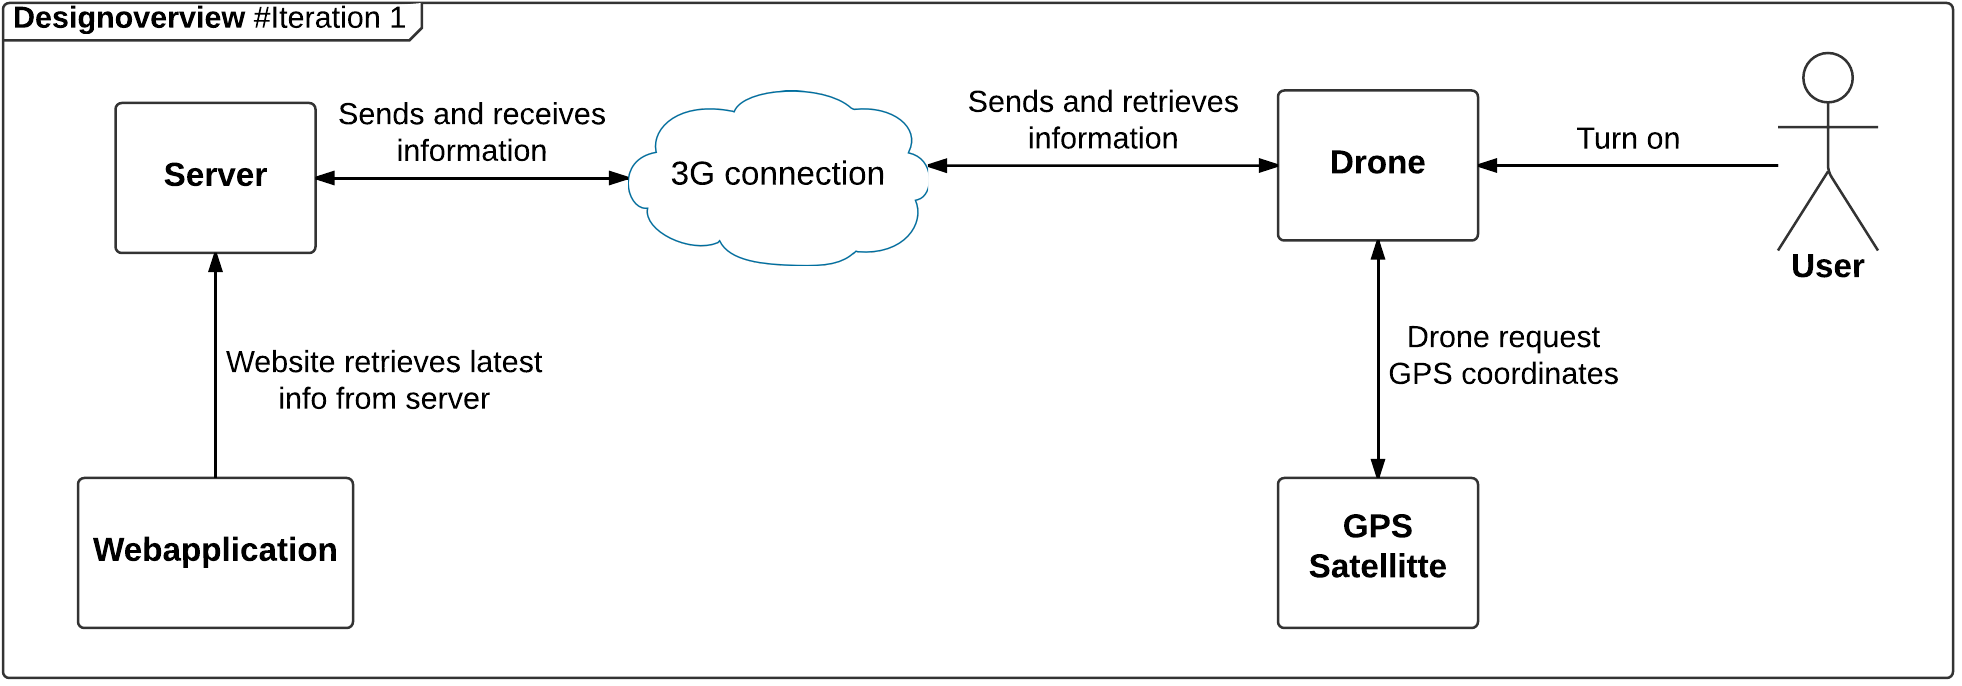
\includegraphics[width=1\textwidth]{Billeder/design_overview/design_overview_iteration1.png}
	\vspace{-.5cm}
	\caption{Design overview \#iteration 1}
	\label{fig:design_overview_UC1}
\end{figure}


\newpage
\subsubsection*{Pakkediagram drone}

I dette afsnit vises pakkediagram tilhørende drone. De pakker der vises i pakkediagrammet består af en eller flere klasser, der med stort samspil udfører opgaver indenfor et fælles ansvarsområde. På hver pakke findes en lille beskrivelse, der tydeliggør pakkens ansvarsområde. 


\begin{figure}[H]
	\centering
	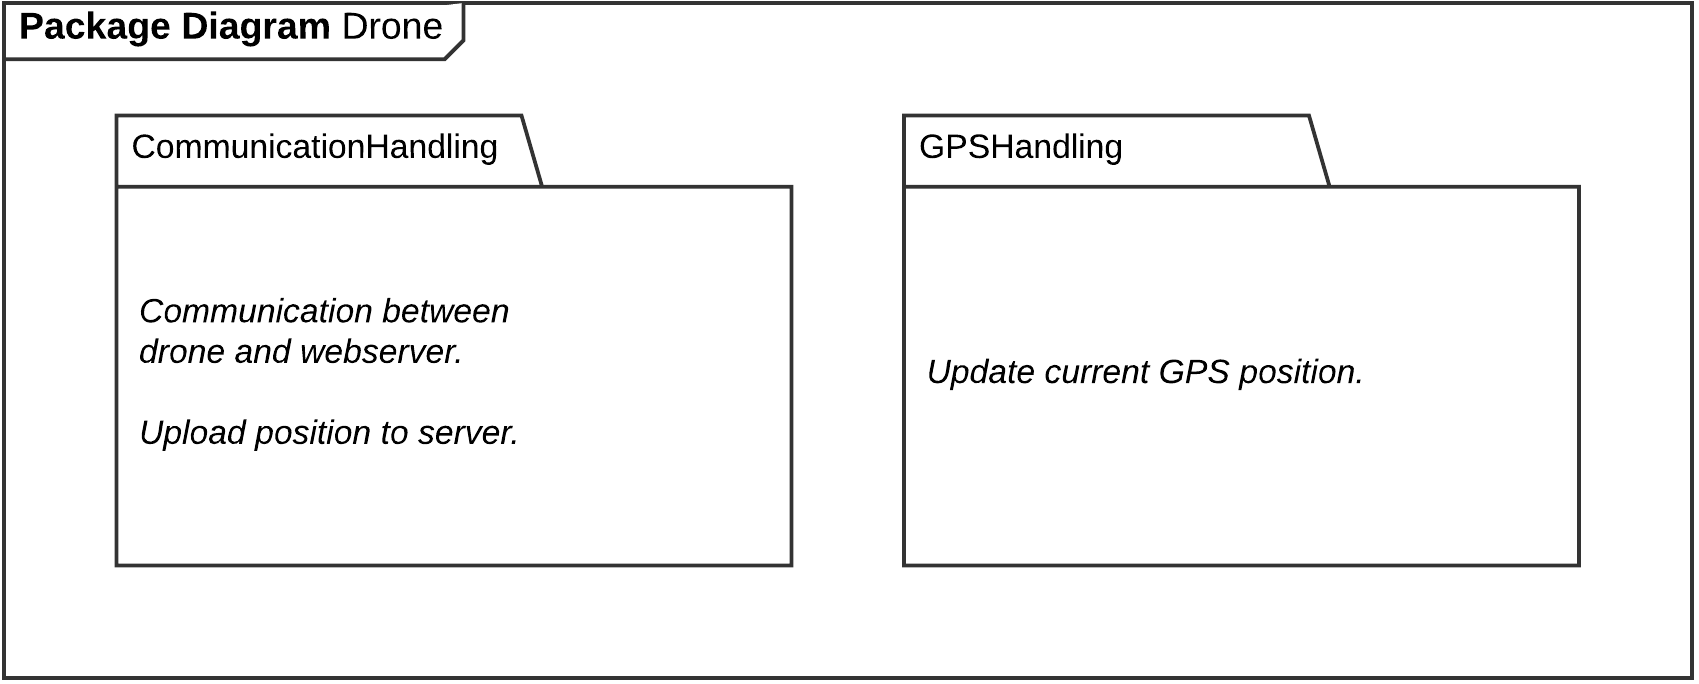
\includegraphics[width=1\textwidth]{Billeder/pakke_diagrammer/iteration1_drone.png}
	\vspace{-0.5cm}
	\caption{Pakkediagram drone}
	\label{fig:iteration1_pakke_diagram_drone}
\end{figure}

\textbf{CommunicationHandling}\\
Pakkens ansvar er kommunikation imellem drone og server. I denne iteration er der fokus på, at dronen skal kunne sende sin nuværende GPS position til server.

\textbf{GPSHandling}\\
Pakkens ansvar er håndtering af GPS. Dels er pakken ansvarlig for opstart og initiering af GPS, og desuden bruges pakken hver gang dronens nuværende GPS position skal opdateres.

\newpage
\subsubsection*{Pakkediagram webapplikation}

I dette afsnit vises pakkediagram tilhørende webapplikationen. De pakker der vises i pakkediagrammet består af en eller flere klasser, der med stort samspil udfører opgaver indenfor et fælles ansvarsområde. På hver pakke findes en lille beskrivelse, der tydeliggør pakkens ansvarsområde. 

\begin{figure}[H]
	\centering
	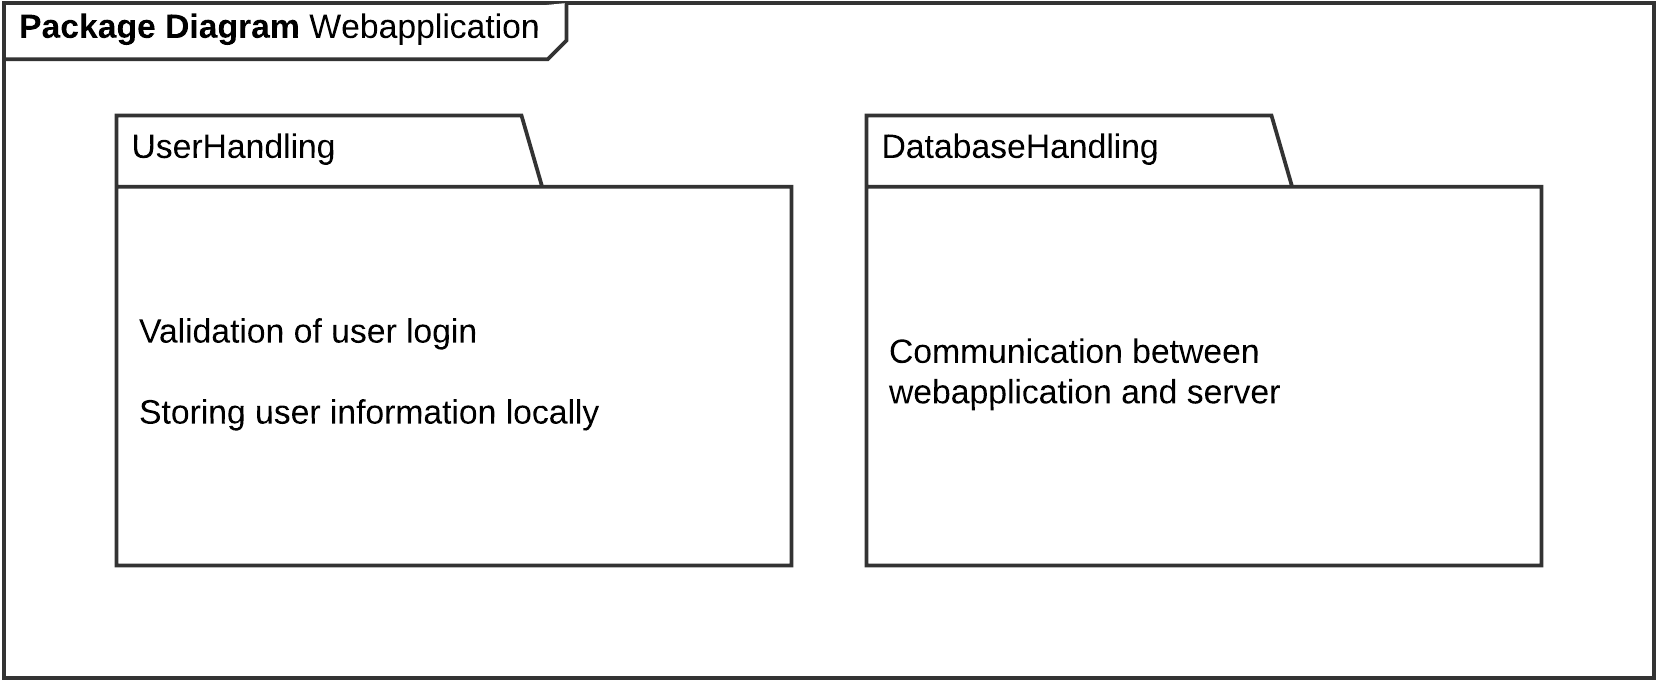
\includegraphics[width=1\textwidth]{Billeder/pakke_diagrammer/iteration1_server.png}
	\vspace{-0.5cm}
	\caption{Overordnet pakke diagram over webapplikationen}
	\label{fig:iteration1_pakke_diagram_webapp}
\end{figure}

\textbf{UserHandling}\\
Pakkens ansvar er validering af login/log ud på websitet. Pakken har også ansvaret for at hente og gemme data om den pågældende bruger.

\textbf{DatabaseHandling}\\
Pakkens ansvar er kommunikation imellem databasen og serveren. 


\newpage
\subsubsection*{Sekvensdiagram drone}
På sekvensdiagrammet på figur \ref{fig:Sekvens_diagram_iteration1}, vises hvilke klasser der indgår og bruges i første iteration. Af sekvensdiagrammet fremgår det, at sekvensen først startes når bruger tilslutter batteri og tænder dronen. Når der er tilkoblet forsyning initialiseres main controller samt 3G/GPS og nuværende GPS position  (longitude og latitude) opdateres. Dronens nuværende GPS position opdateres når dronen sender PUT requests til websitet. PUT requests bruges dels til at fortælle websitet at dronen er online og dels til at give websitet information om dronens nuværende position. 

%kommentar
\begin{figure}[H]
	\centering
	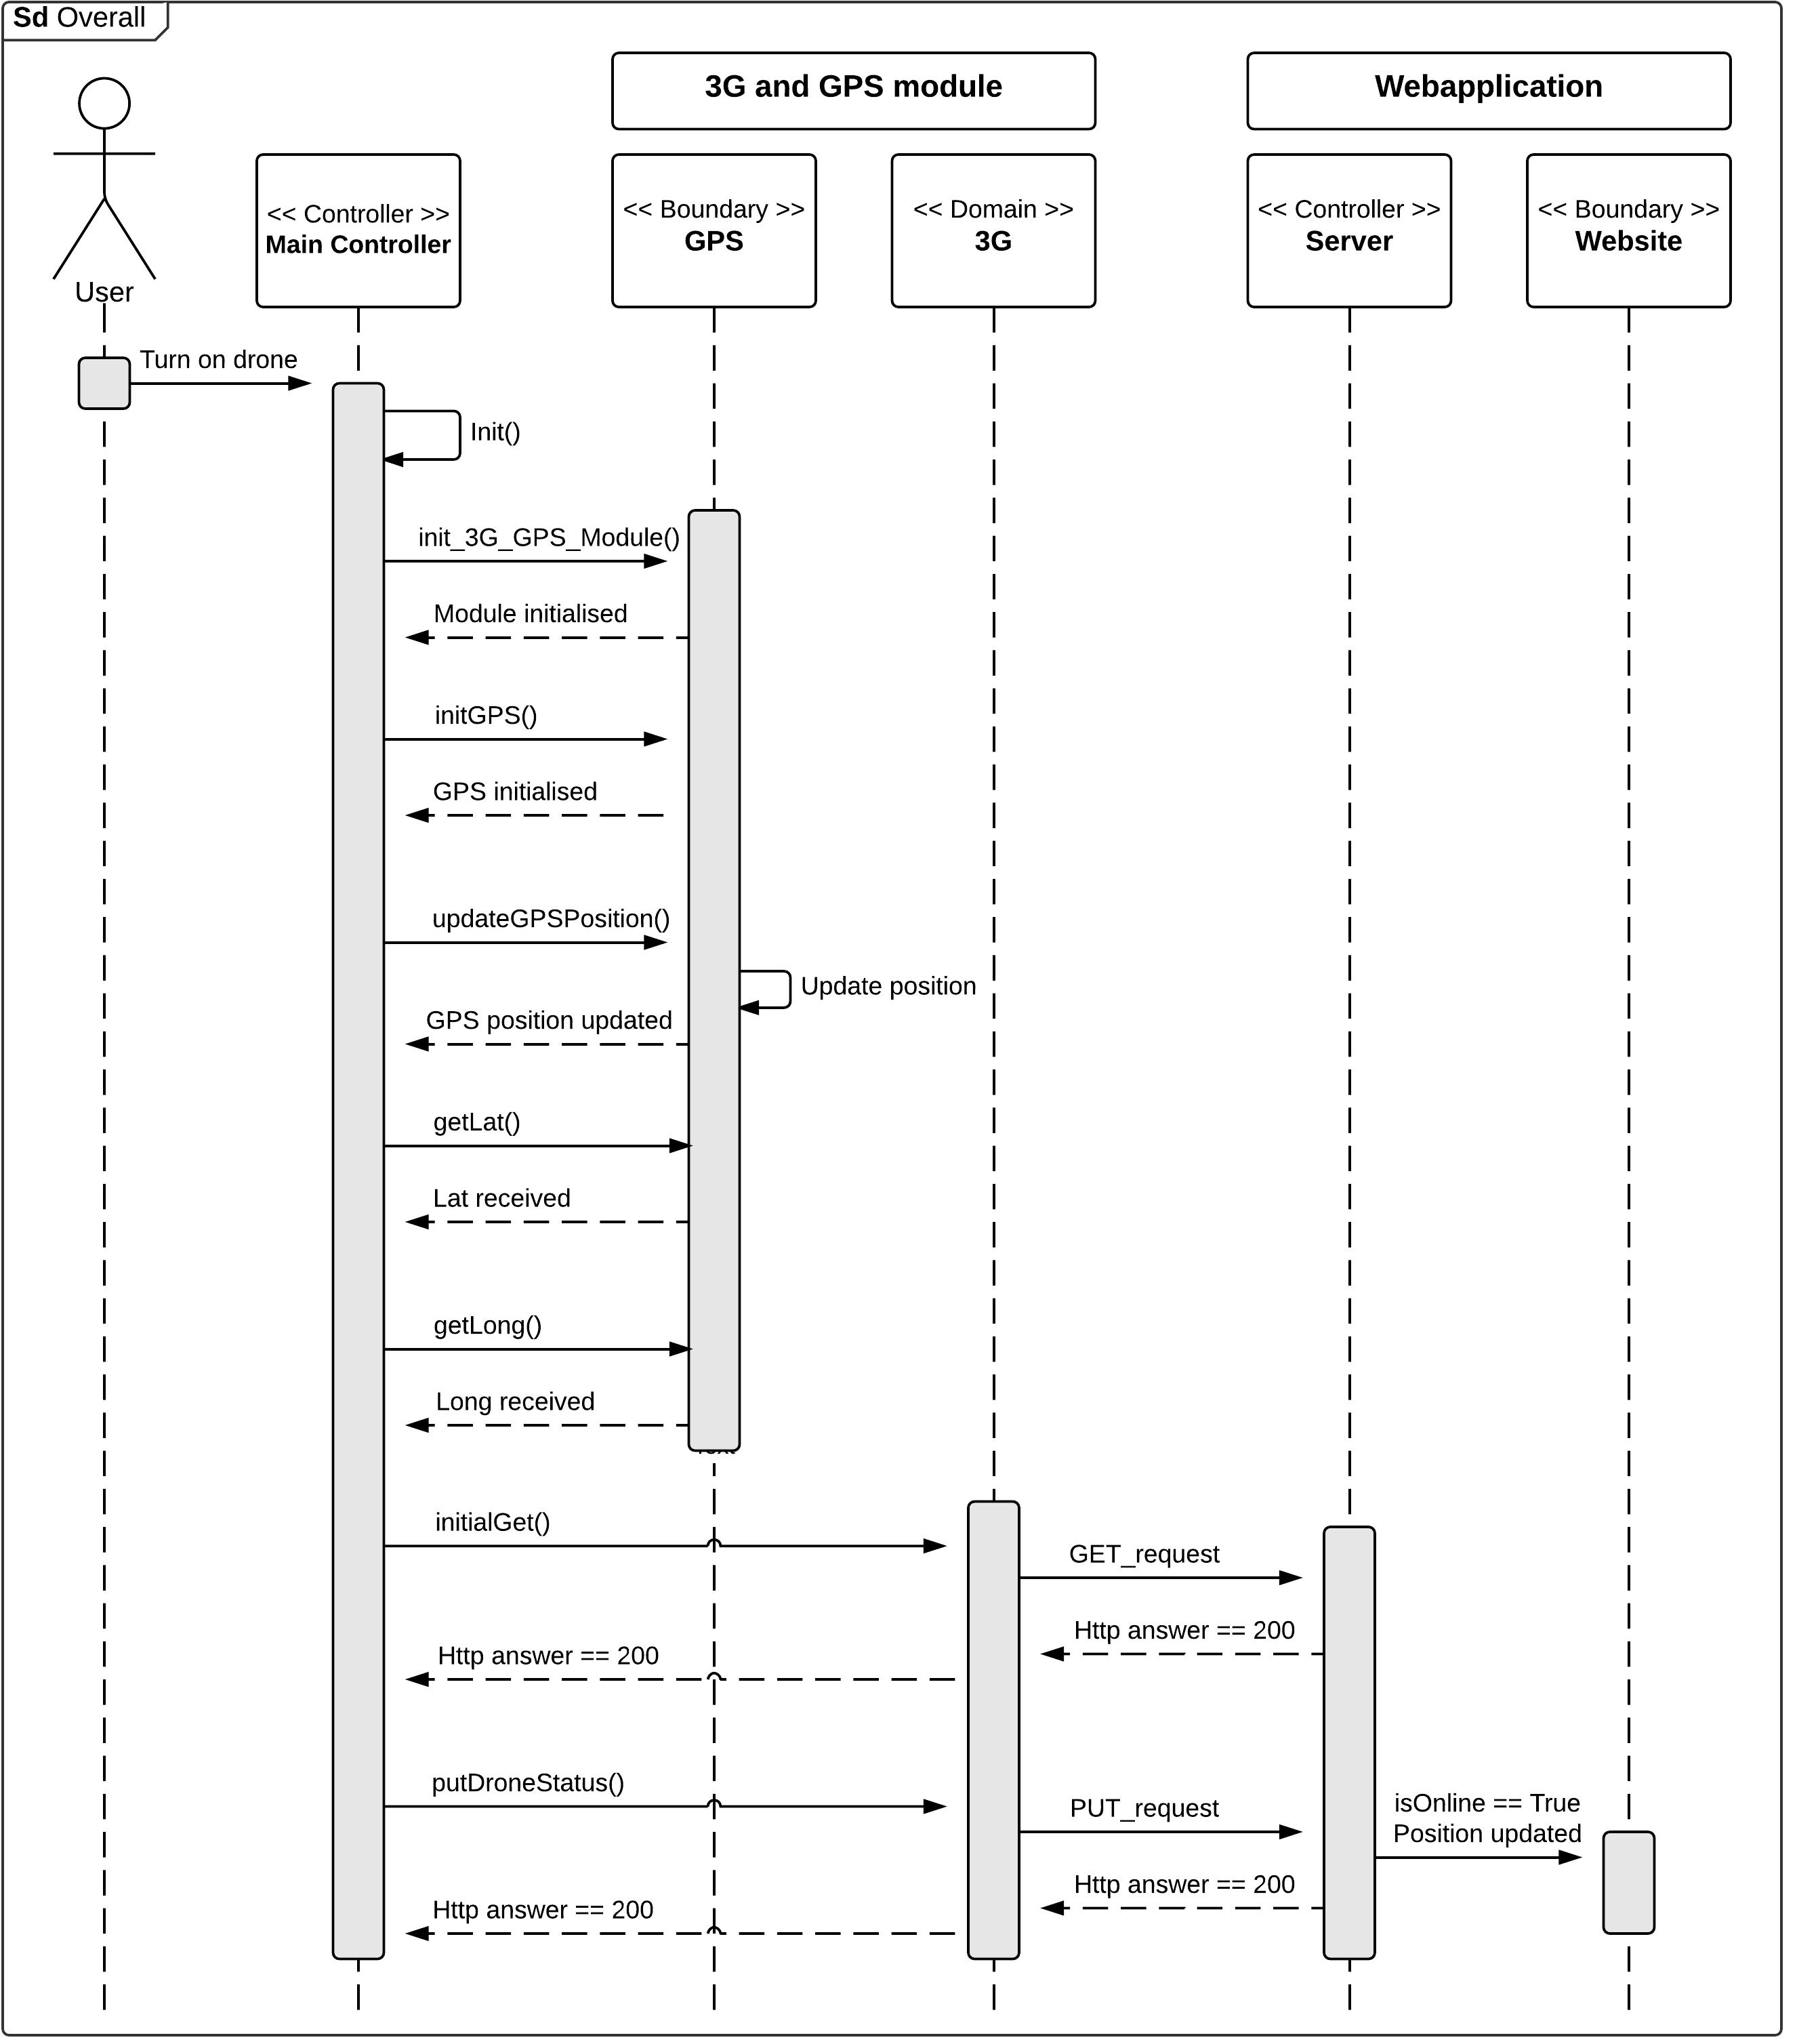
\includegraphics[width=1\textwidth]{Billeder/sekvens/sekvens_iteration1}
	\caption{Sekvens diagram \#iteration 1}
	\label{fig:Sekvens_diagram_iteration1}
\end{figure}
\newpage

På figur \ref{fig:Sekvens_diagram_initialget} og figur \ref{fig:Sekvens_diagram_putDroneStatus} bliver 3G modulet yderligere uddybet.\\
\ref{fig:Sekvens_diagram_initialget} viser hvilke klasser der anvendes til at hente data fra serveren. 

\begin{figure}[H]
	\centering
	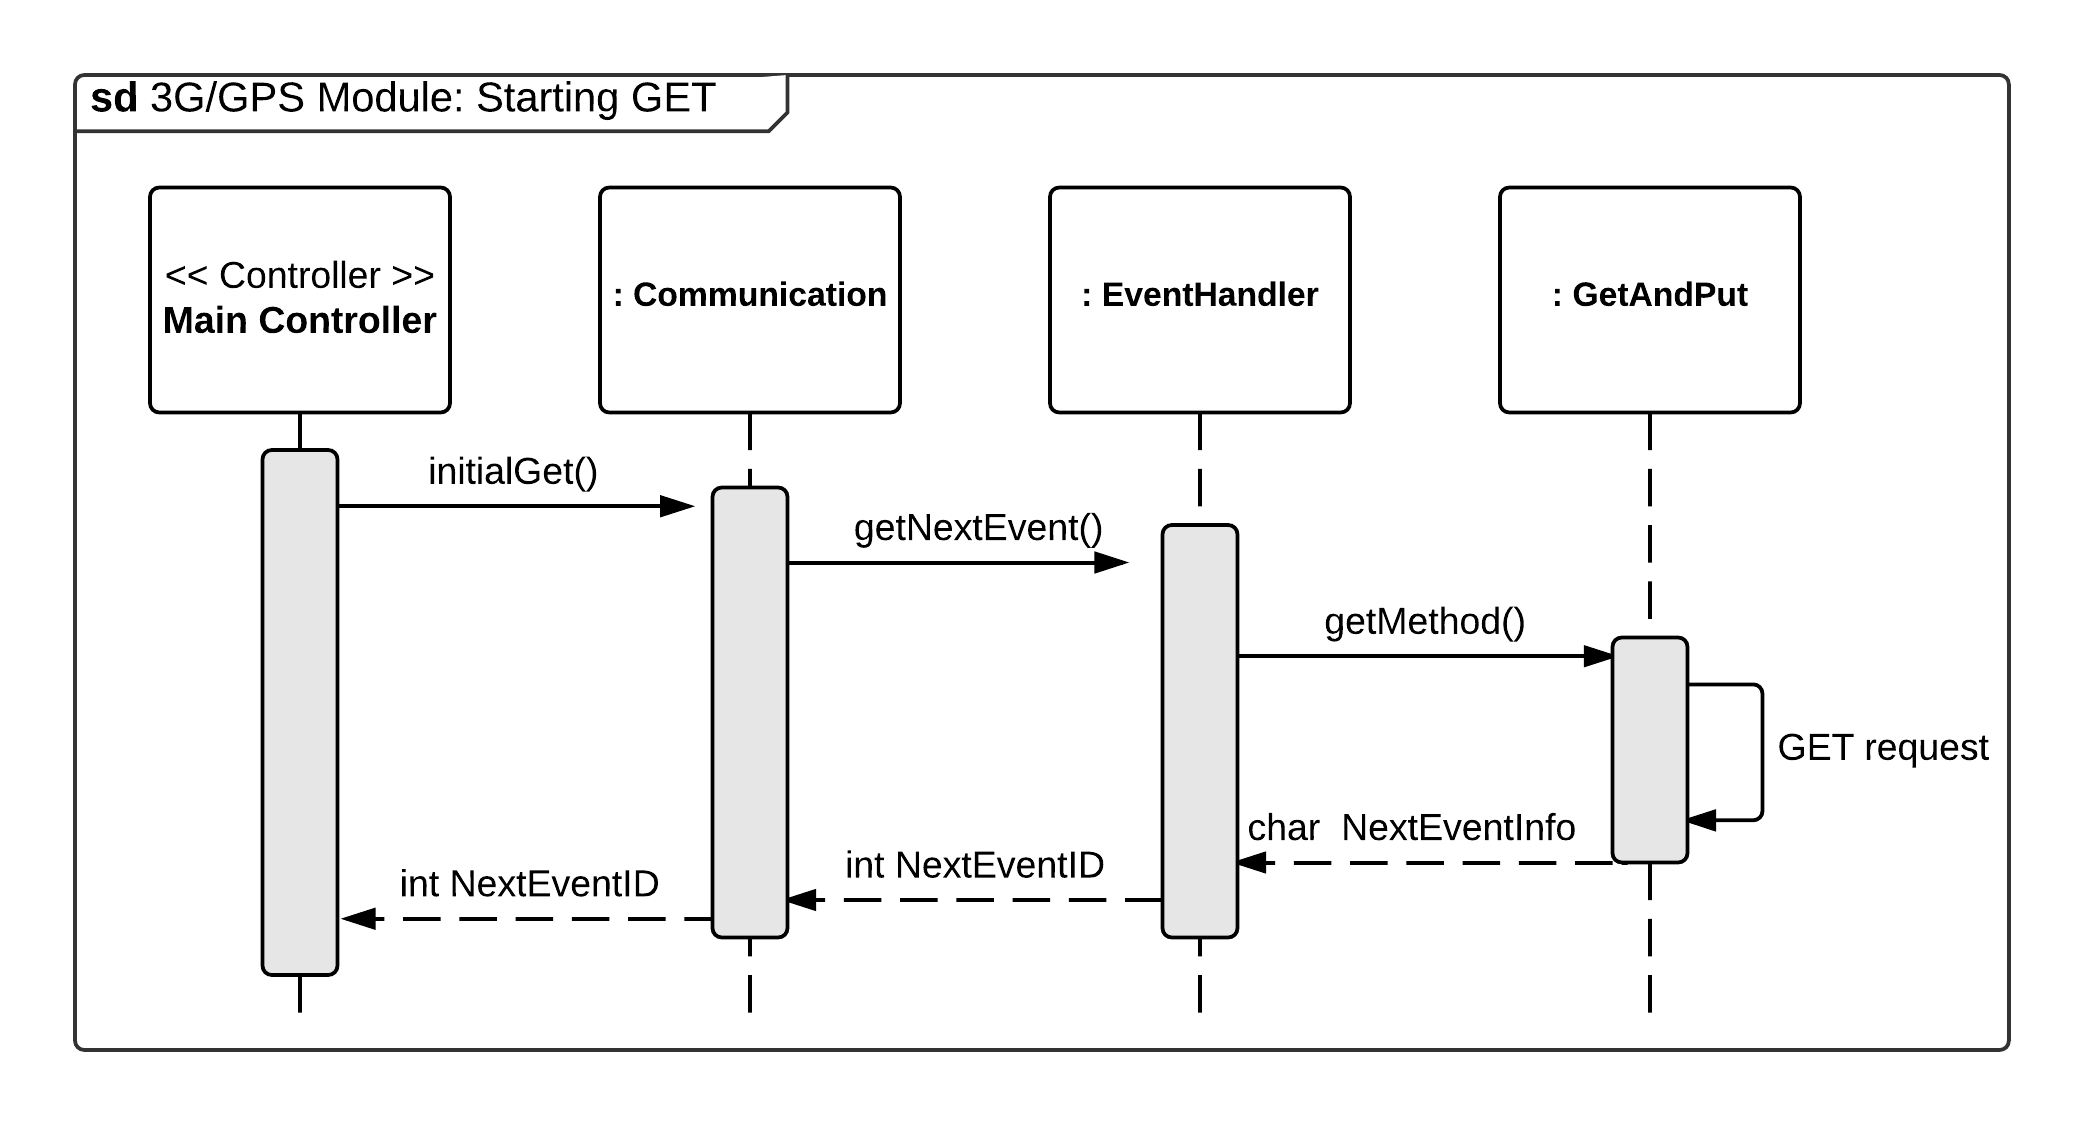
\includegraphics[width=1\textwidth]{Billeder/sekvens/sekvens_iteration1_initialget}
	\caption{Sekvens diagram \#iteration 1 - initialget}
	\label{fig:Sekvens_diagram_initialget}
\end{figure}

\vspace{.5cm}

De data der hentes med GET requestet, bruges sammen med PUT requestet. For at kunne udføre et PUT request, skal data der ønskes sendt til server stemme overens med det data der i forvejen ligger på serveren.

\begin{figure}[H]
	\centering
	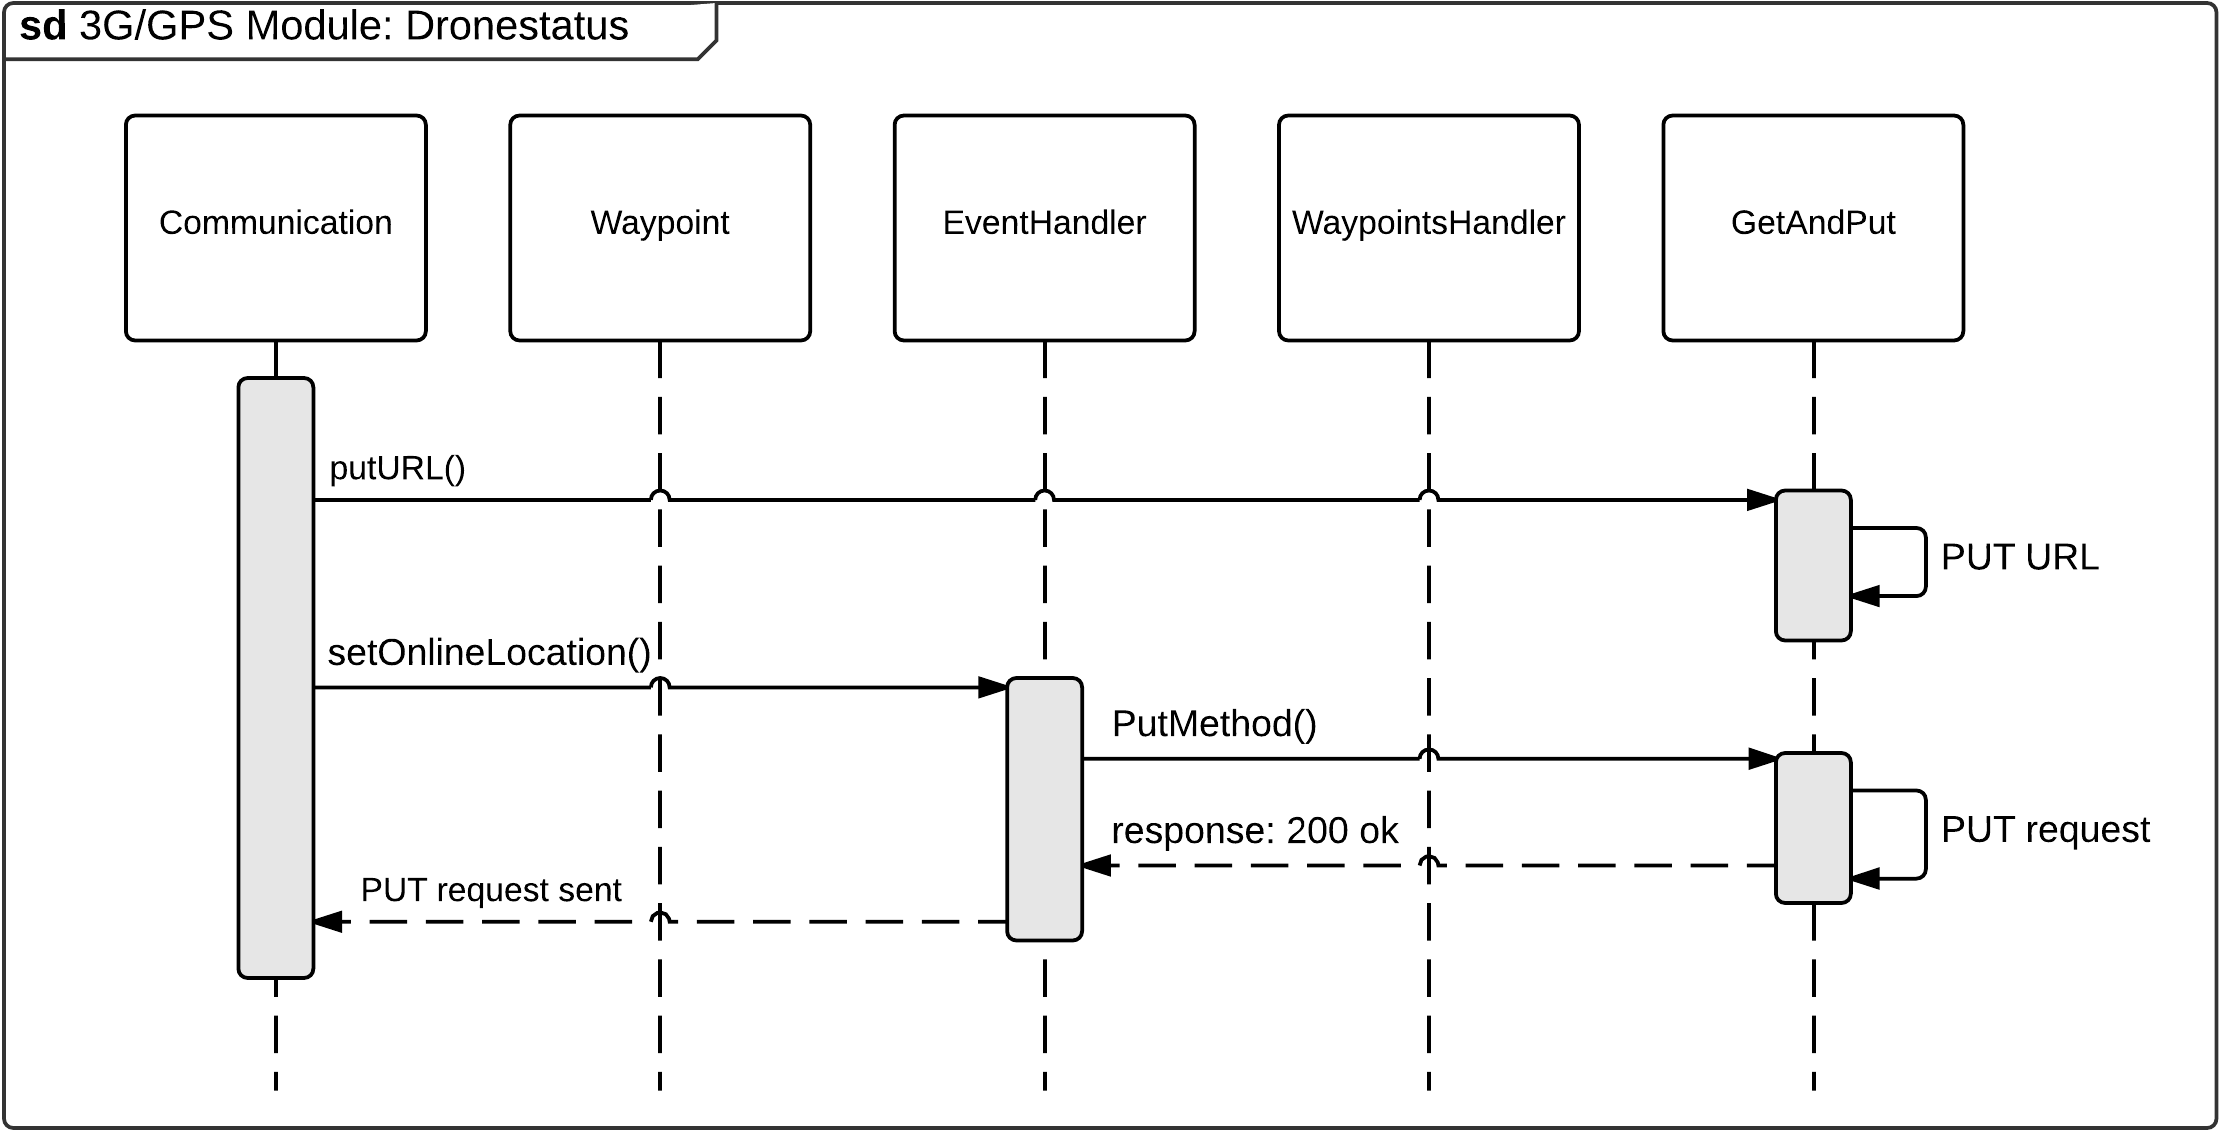
\includegraphics[width=1\textwidth]{Billeder/sekvens/sekvens_iteration1_putdronestatus}
	\caption{Sekvens diagram \#iteration 1 - putDroneStatus}
	\label{fig:Sekvens_diagram_putDroneStatus}
\end{figure}


\newpage

\subsubsection*{Sekvensdiagram webapplikation}
På figur \ref{fig:Sekvens_diagram_login} ses sekvens diagrammet over login på webappplikationen. På diagrammet vises det at useren først bliver ført til næste side ved succesfuld login. Diagrammet viser også kommunikationen med CRUDServiceDrone som kommunikerer med databasen. Diagrammet viser også hvordan AuthenticationServices setter den givet users data inden useren bliver ført vider i systemet.

\begin{figure}[H]
	\centering
	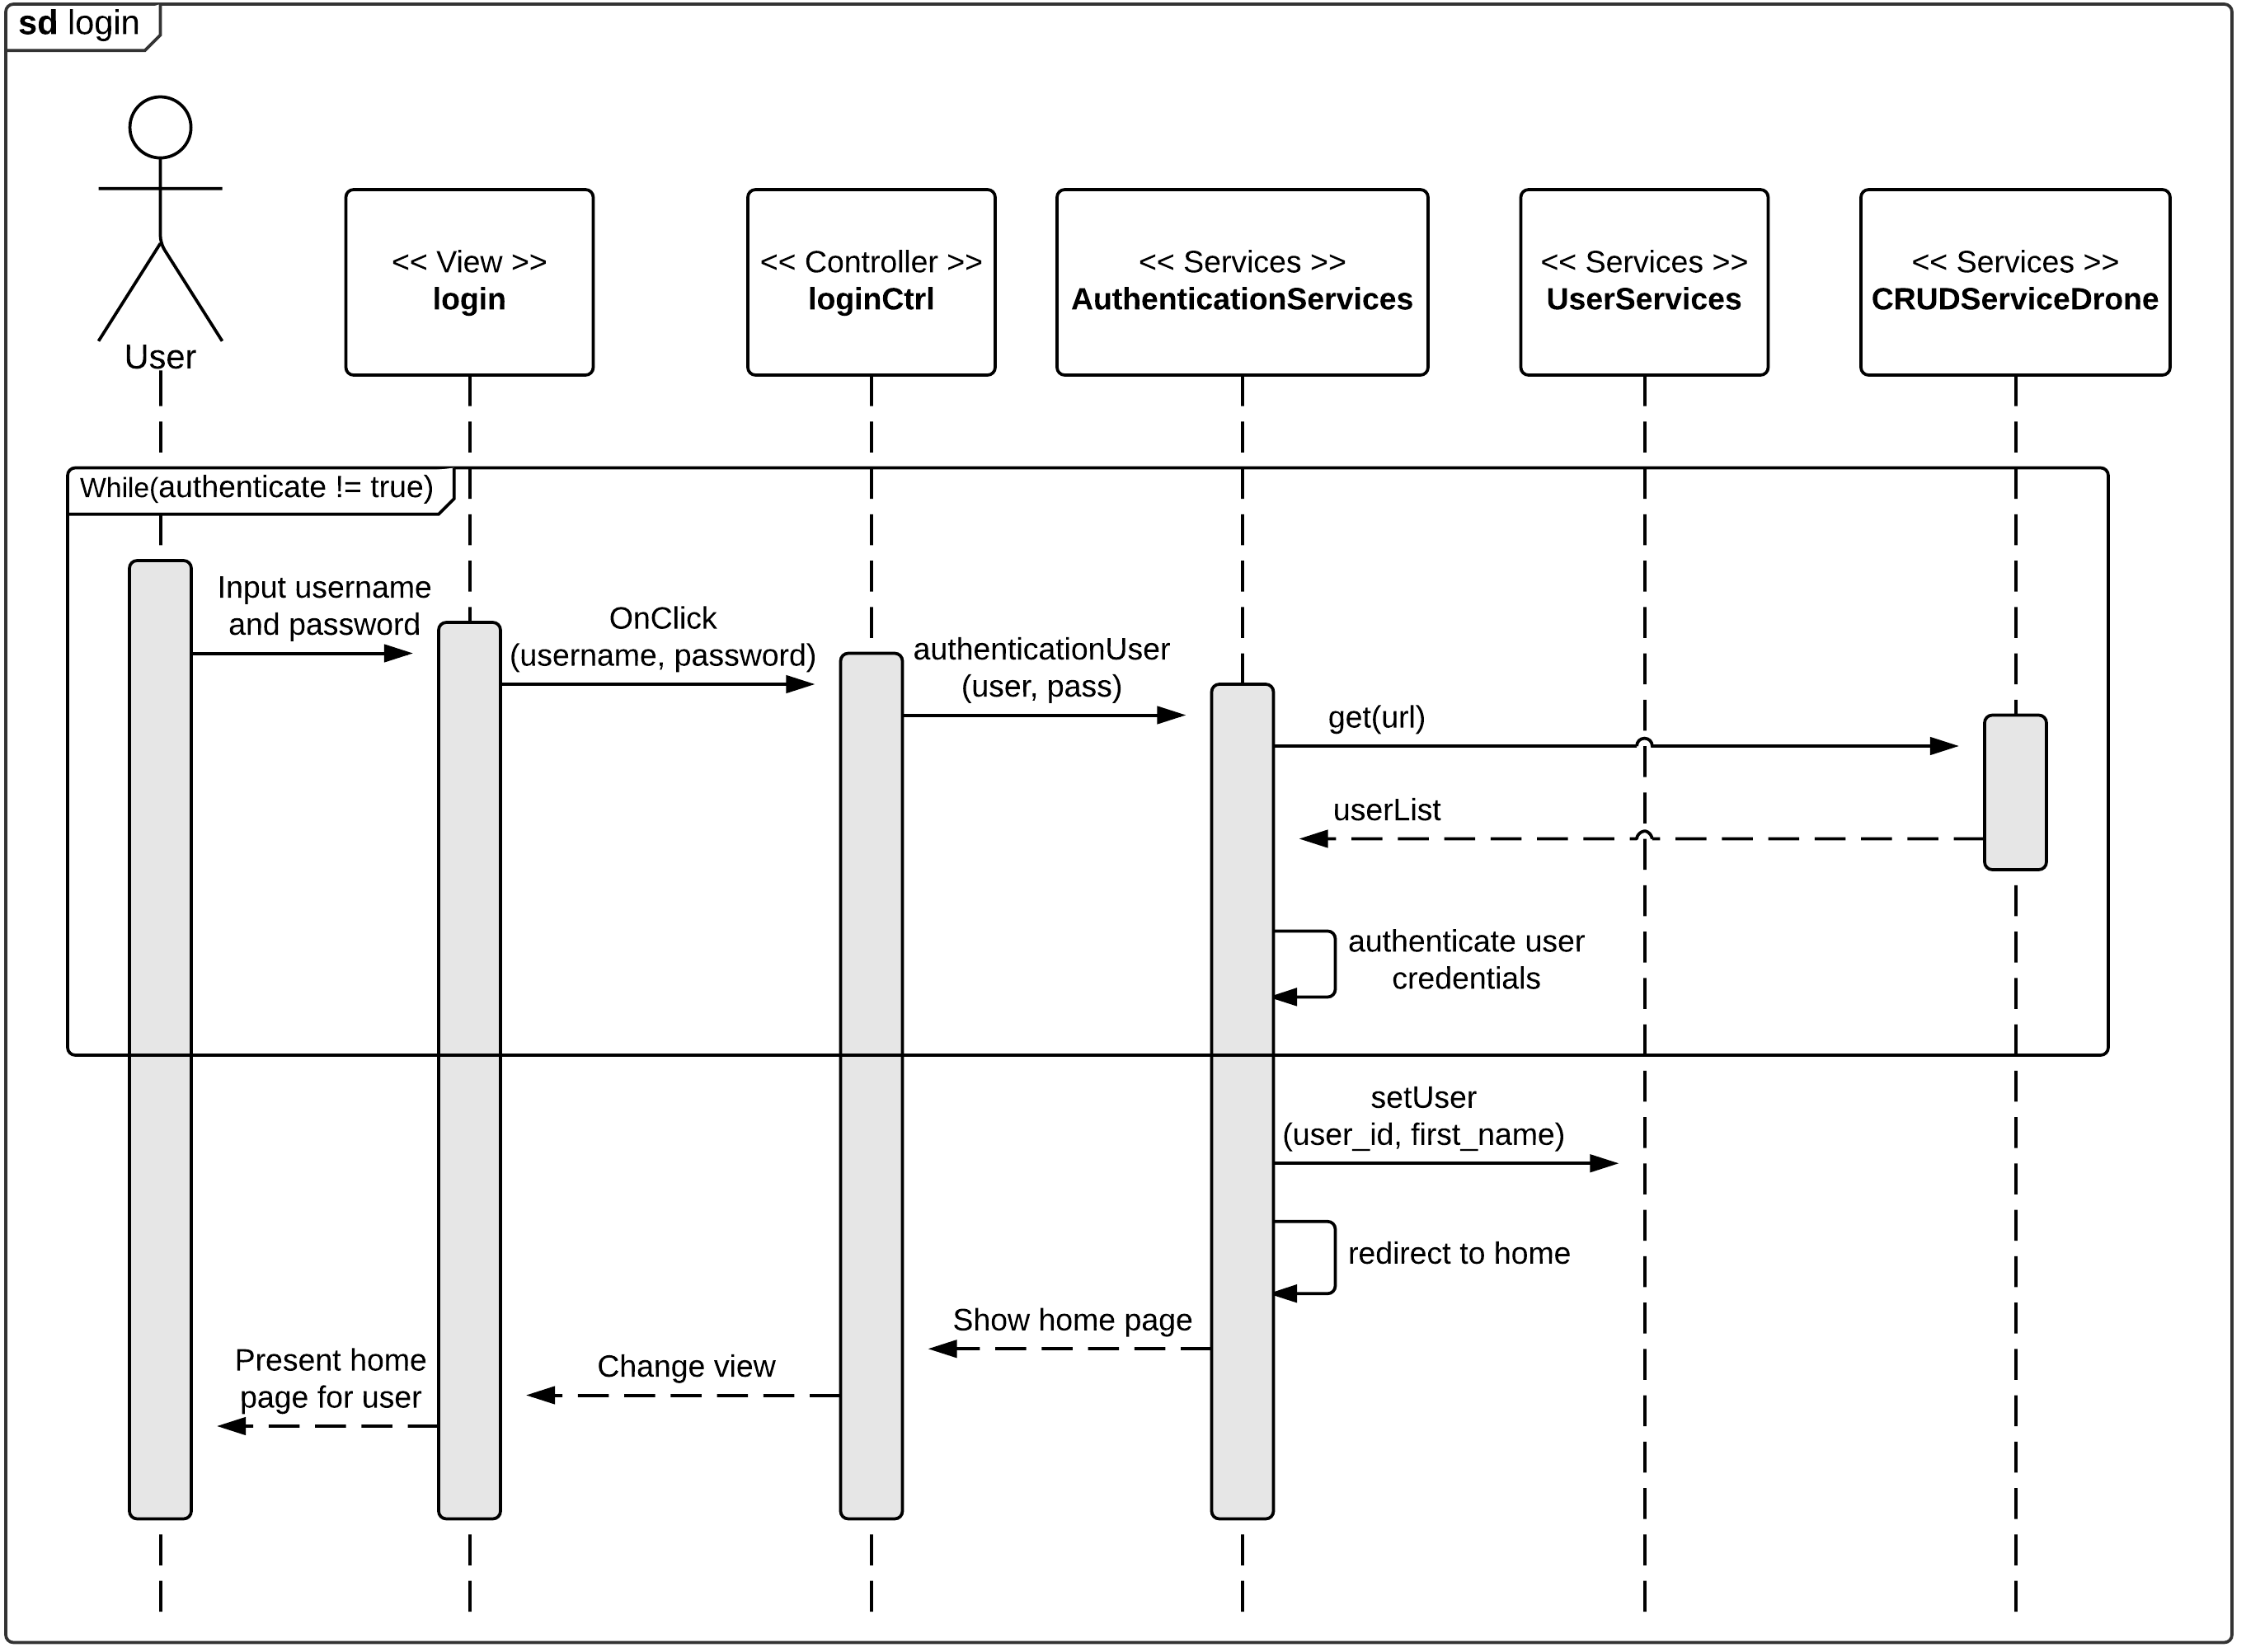
\includegraphics[width=1\textwidth]{Billeder/sekvens/login_sq_diagram.png}
	\caption{Sekvens diagram login}
	\label{fig:Sekvens_diagram_login}
\end{figure}
\newpage


\subsubsection*{Klassediagram drone}
\vspace{-0.2cm}
Figur \ref{fig:classDiagram_iteration1} vises et klassediagram tilhørende iteration 1. Klassediagrammet viser iterationens vigtigste klasser, samt deres tilhørende metoder og attributter. På den følgende side forefindes en kort beskrivelse klasserne og deres metoder.

\vspace{-0.2cm}
%kommentar
\begin{figure}[H]
	\centering
	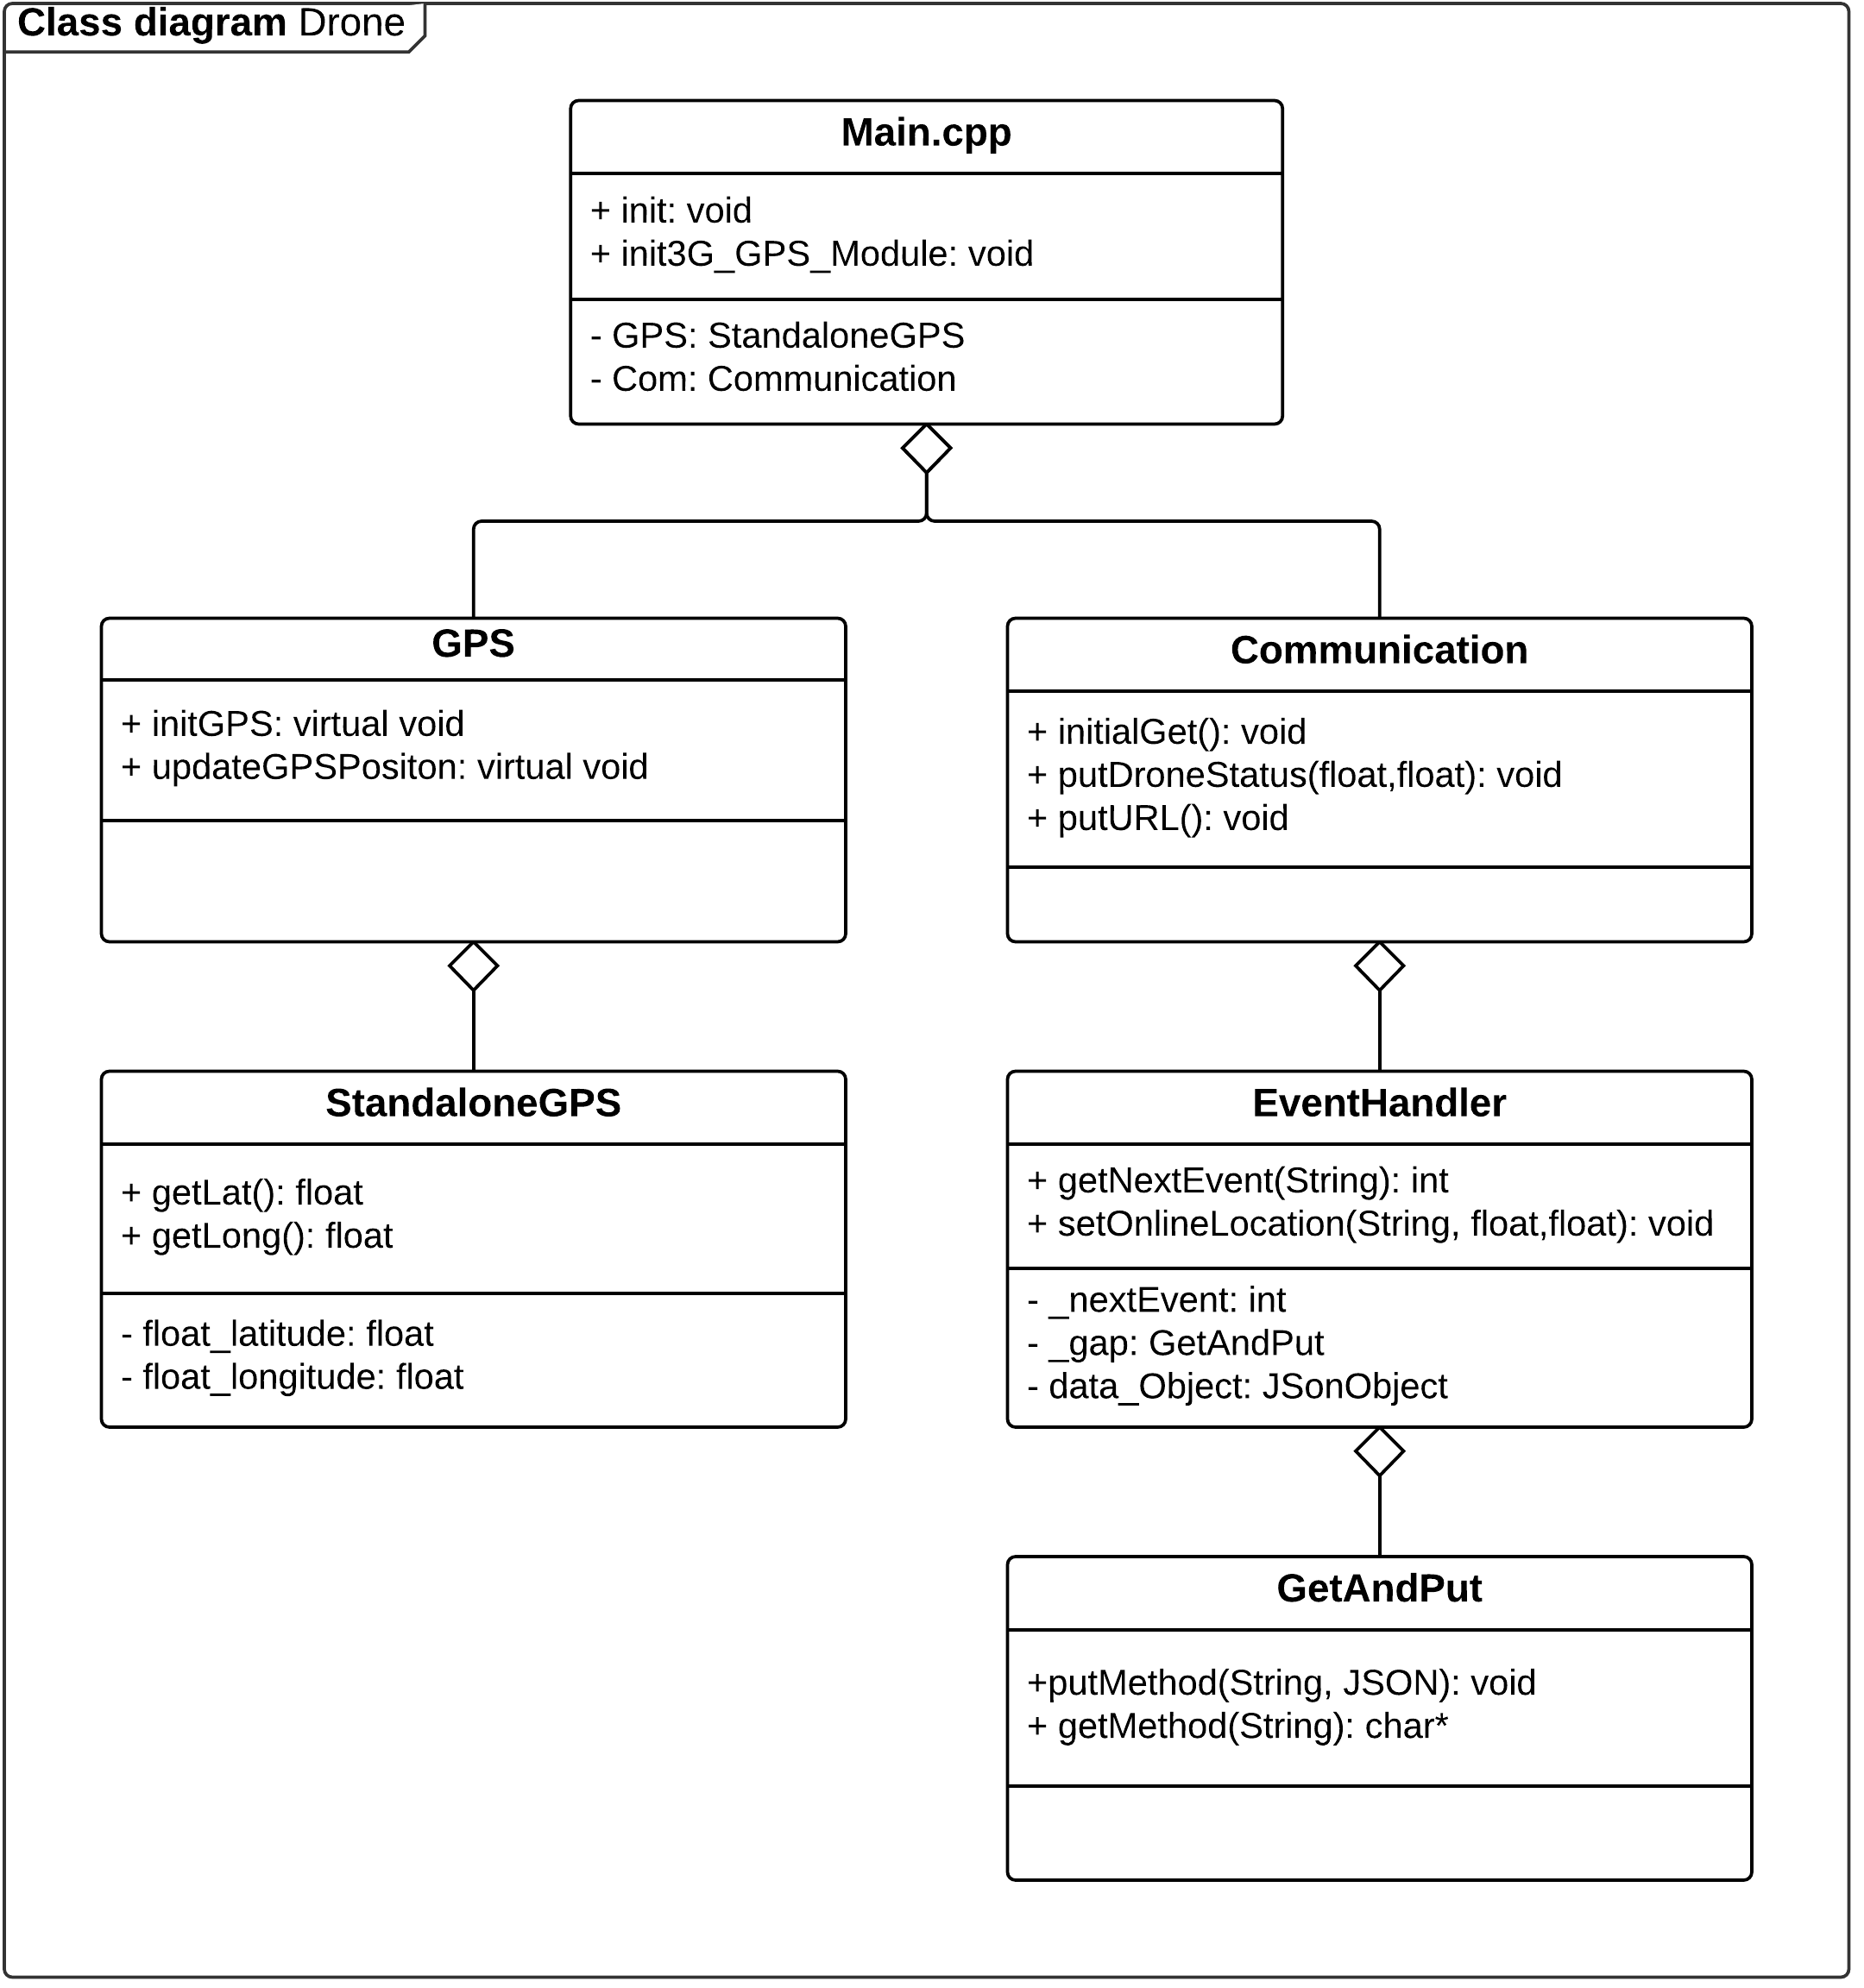
\includegraphics[width=1\textwidth]{Billeder/klasse_diagrammer/classdiagram_iteration1.png}
	\vspace{-0.5cm}
	\caption{Klassediagram \#iteration 1}
	\label{fig:classDiagram_iteration1}
\end{figure}
\vspace{-0.1cm}

\textbf{Main.cpp} \\
Main.cpp filen bruges til at sætte arduino board korrekt op, bla. sættes baudrate på de forskellige serielle forbindelser. Desuden bruges Main.cpp til at kalde og eksekverer forskellige klasse, objekter og funktioner.

\textbf{GPS} \\
GPS klassen er implementeret som en abstract klasse, idet den ikke selv har nogle metoder den skal bruge, men med virtuelle metoder der sikrer at de implementeres i de afledte klasser. 
Init og updateGPSPosition er valgt til at være virtuelle klasser, hvilket gør at de skal implementeres uanset hvilken GPS der bruges. Klassen er lavet fordi der i udgangspunkt var mulighed for at bruge 3 forskellige slags GPS modes med 3G/GPS shieldet. 

\textbf{StandaloneGPS}\\
Denne klasse er ansvarlig for al kommunikation med GPS'en når standalone mode er valgt. 

\newpage

Nedenfor ses figur \ref{fig:udvidet3G_it1} som er en udvidet klasse diagram over 3G modulet. Klasse diagrammet viser et udvidet klasse diagram, der viser hvilke metoder der indgår i iteration 1 for 3G modulet. 

\begin{figure}[H]
	\centering
	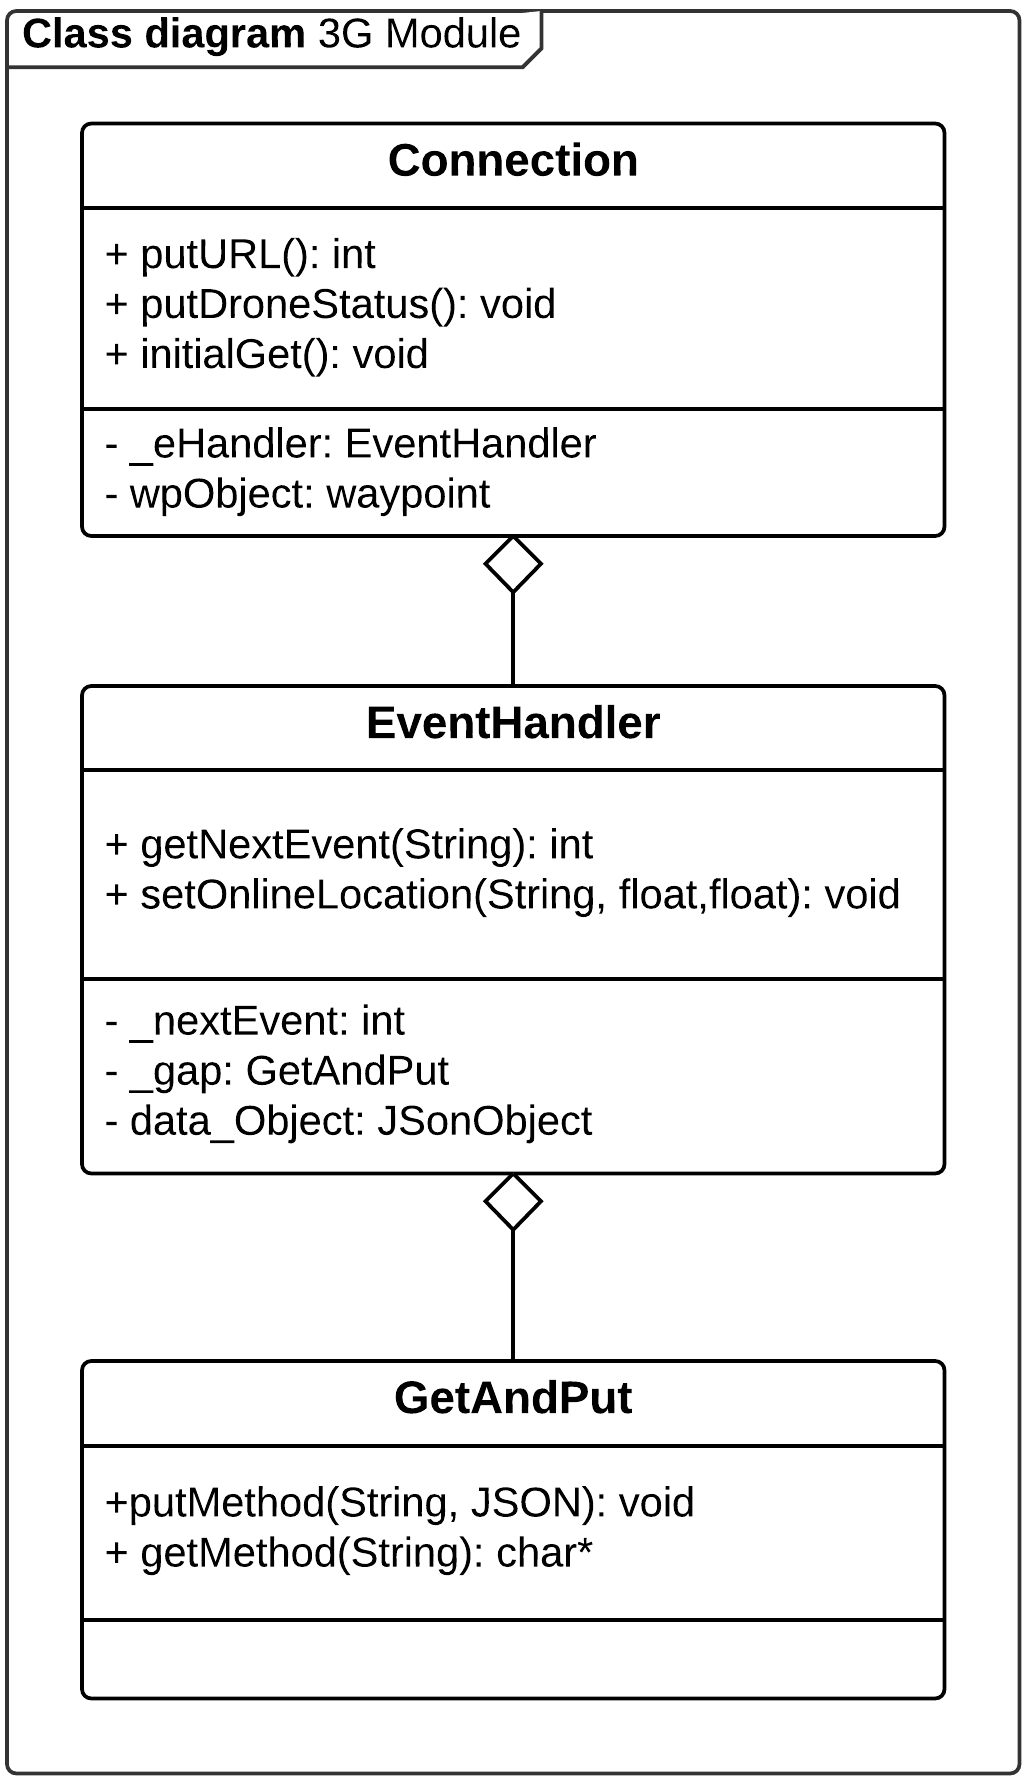
\includegraphics[width=0.50\textwidth]{Billeder/klasse_diagrammer/udvidet3G_iteration1.png}
	\vspace{0.5cm}
	\caption{Udvidet klasse diagram for 3G modulet - iteration 1}
	\label{fig:udvidet3G_it1}
\end{figure}

\textbf{GetAndPut} \\
GetAndPut klassen er den klasse der er tættest på hardwaren. Klassen indeholder de http metoder der bruges til kommunikation mellem dronen og serveren. 

\textbf{Communication} \\
Communication klassen er den øverste klasse og den håndterer sammen med andre klasser, alt der har med 3G at gøre.

\textbf{EventHandler} \\
EventHandleren er den klasse der håndterer Events. EventHandleren er bindeledet mellem communication- og GetAndPut klassen. EventHandleren sorterer eventID'et fra de data den modtager og returnerer værdien til communication klassen. 


\newpage

\subsubsection*{Klassediagram website}
\vspace{-0.2cm}
Figur \ref{fig:classDiagram_login} viser klassediagrammet tilhørende websitet for iteration 1.
\vspace{-0.2cm}
\begin{figure}[H]
	\centering
	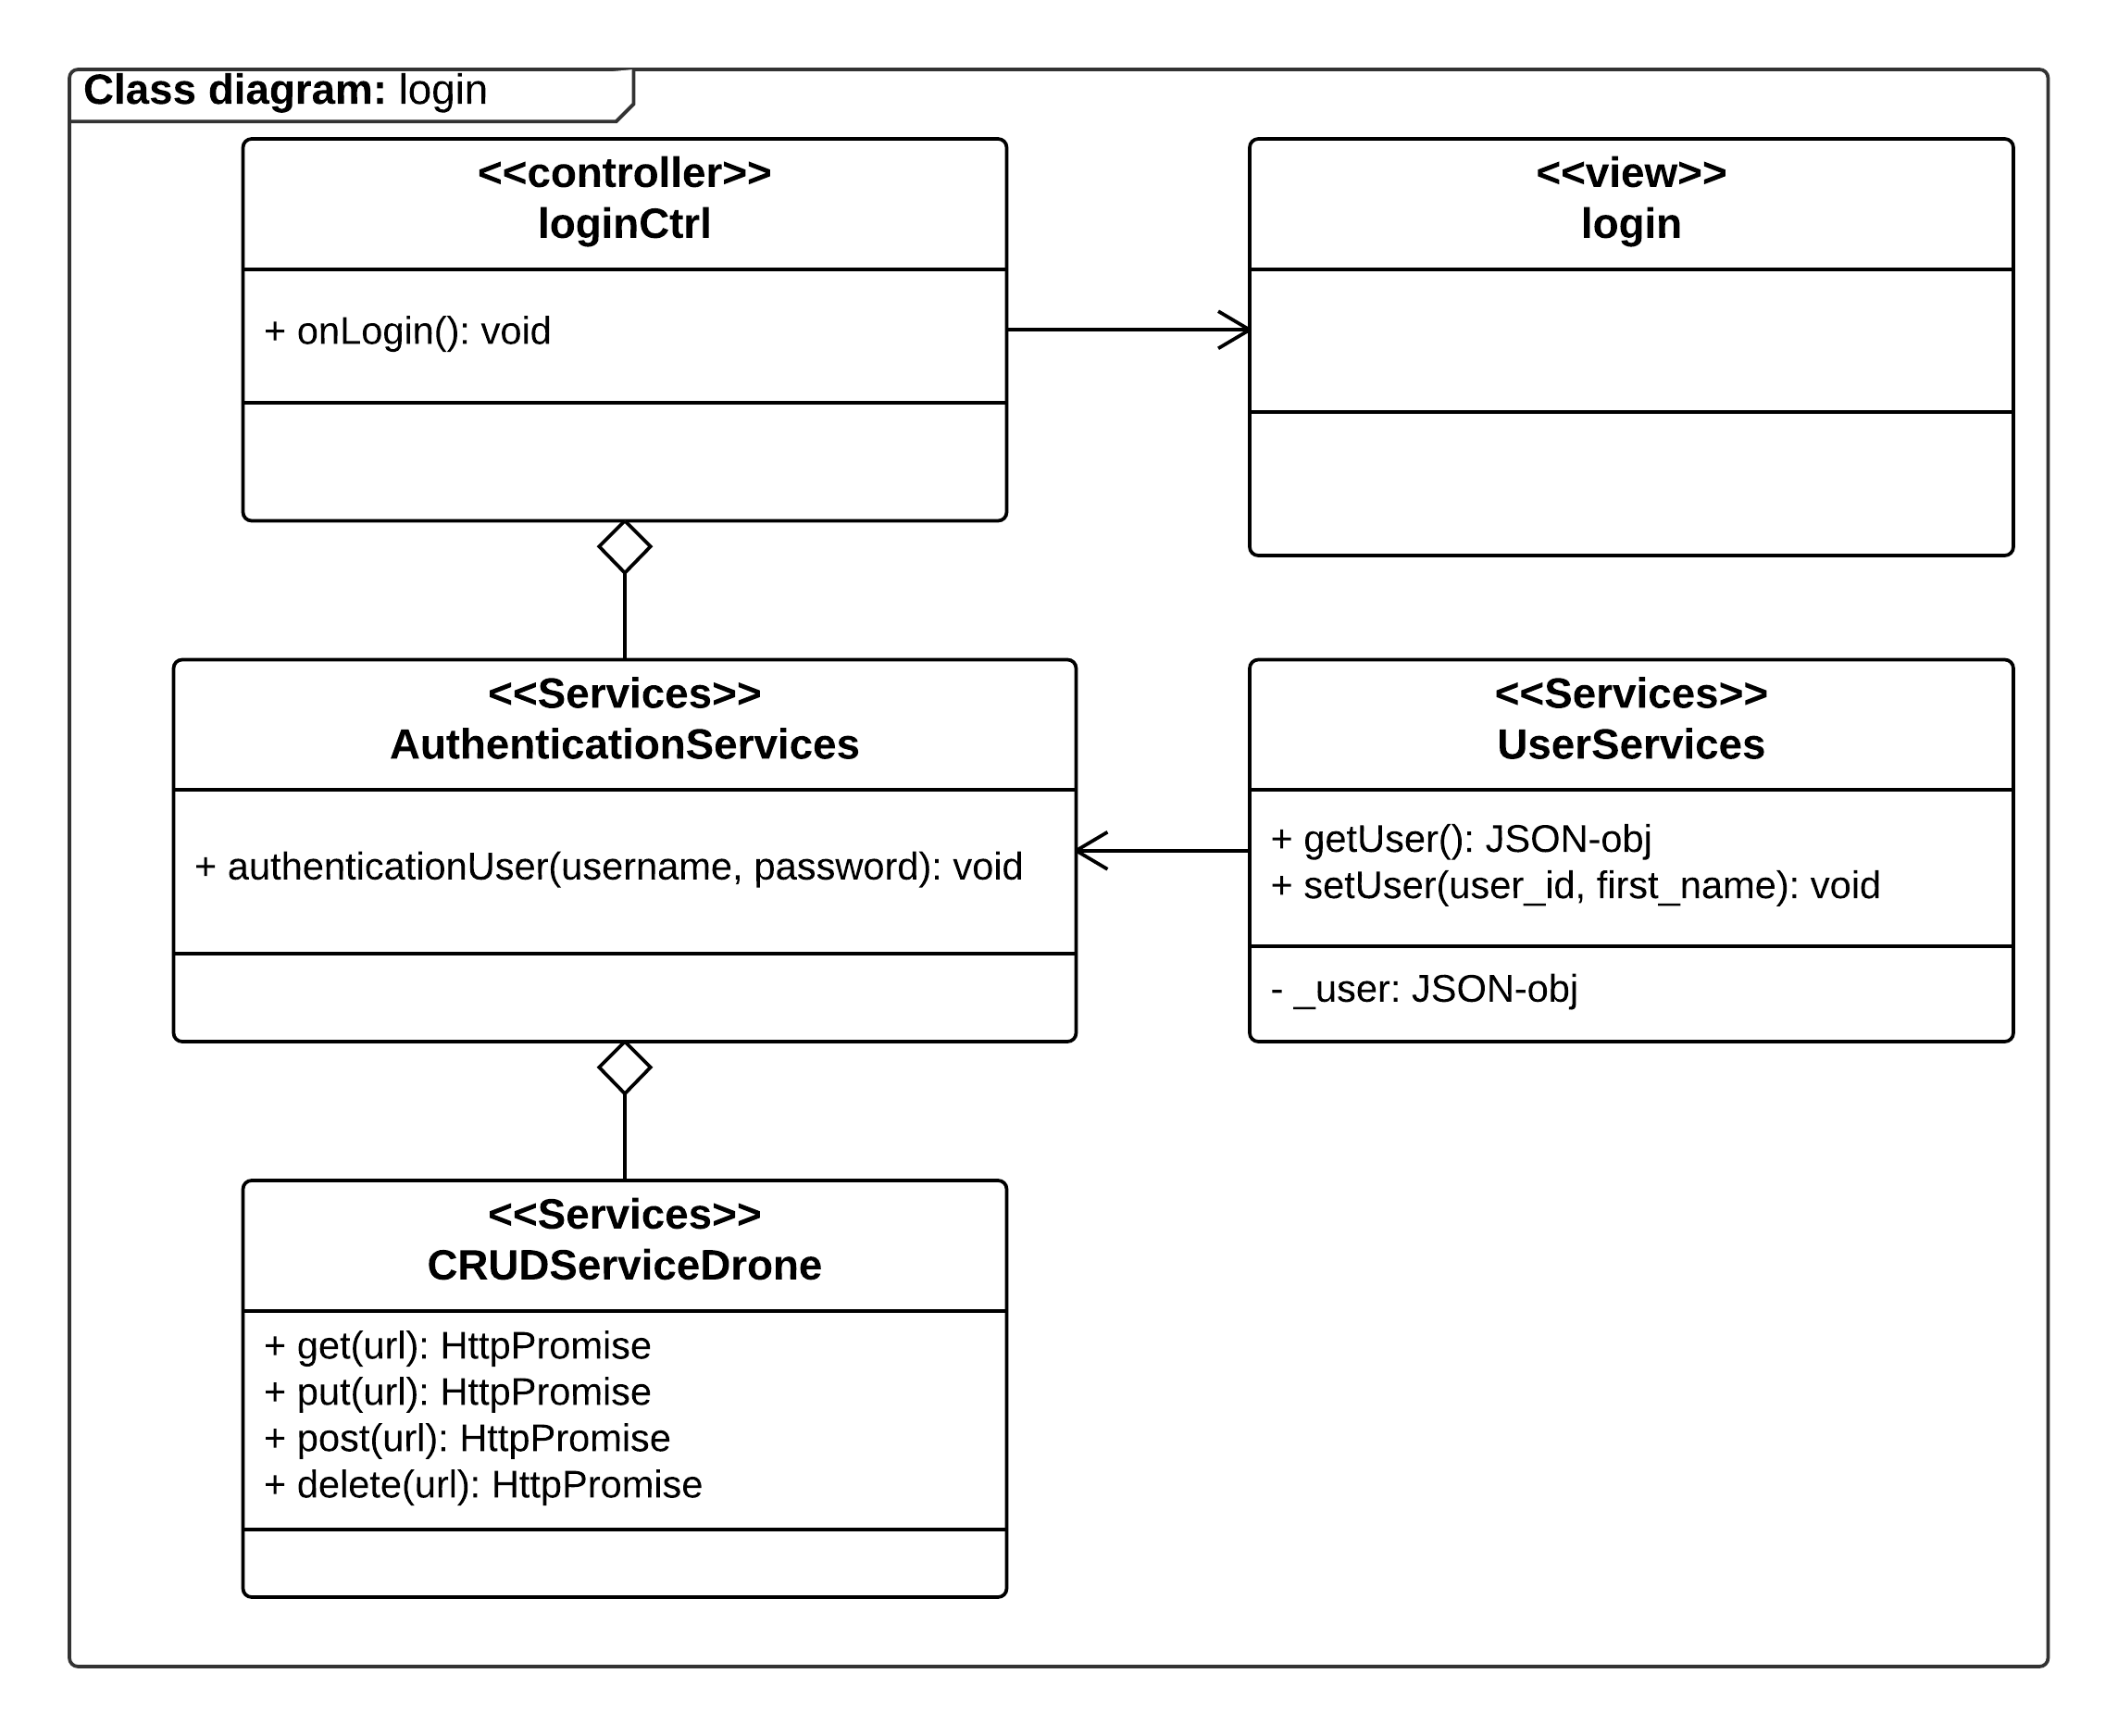
\includegraphics[width=1\textwidth]{Billeder/klasse_diagrammer/login_class_diagram.png}
	\vspace{-0.5cm}
	\caption{Klassediagram login}
	\label{fig:classDiagram_login}
\end{figure}

\vspace{-0.2cm}

\textbf{login} \\
Login view filen er det html script som useren ser på sin webclient. Filen er two-way databinded med loginCtrl klassen. Via denne binding kan der sendes og modtages data direkte.

\textbf{loginCtrl} \\
LoginCtrl er controller klassen som er forbundet med view klassen via two-way databinding. Klassen uddelegere også opgaver til dens services.

\textbf{AuthenticationServices} \\
AuthenticationServices er en service der afgør om user er authenticated eller ej. Hvis user er authenticated bliver han redirected til websitets home-page. Klassen gør brug af UserServices til at gemme information om den user der er logget ind i systemet.

\textbf{UserServices}\\
UserServices indeholder information om user der er logget ind i systemet.

\textbf{CRUDServiceDrone} \\
CRUDServiceDrone er den service der styre alt kontakt til databasen i systemet. Igennem denne service er det muligt at hente, opdater og poste data til databasen.


\subsubsection*{State machine diagram}
\vspace{-0.1cm}
I state machine diagrammet på figur \ref{fig:Statemachine_iteration1}, vises de forskellige states der eksisterer i iteration 1 og hvordan flowet imellem dem ser ud. Der eksisterer givet vis kun 2 states i iteration 1, men state machinen er medtaget fordi den på nem og overskuelig vis illustrerer systemflowet.
%kommentar
\begin{figure}[H]
	\centering
	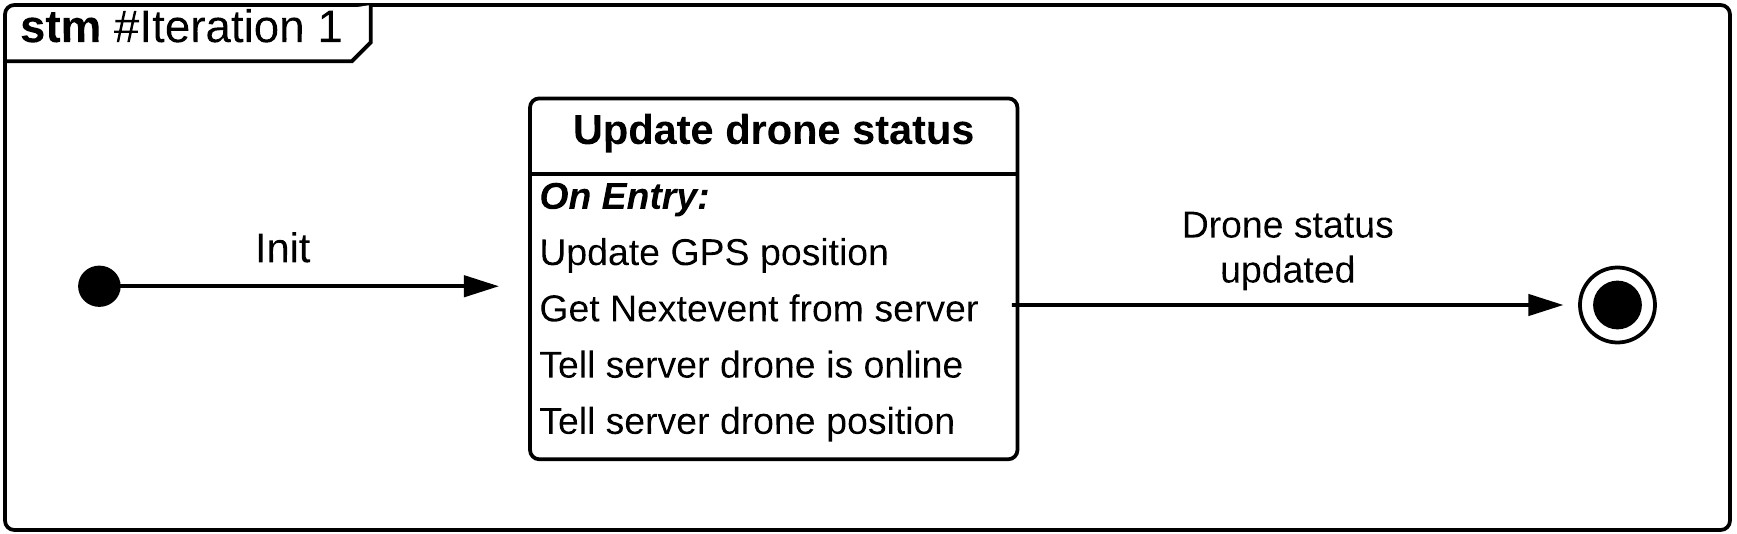
\includegraphics[width=1\textwidth]{Billeder/statemachine/State_iteration1.png}
	\vspace{-0.5cm}
	\caption{Statemachine \#iteration 1}
	\label{fig:Statemachine_iteration1}
\end{figure}

\newpage
\subsection{Iteration \#2}
I iteration 2 er formålet at færdiggøre funktionalitet på websitet så det muliggøres at oprette nye waypoints til dronen og at muliggøre autonome flyvning. Bruger skal kunne oprette flyveopsætninger og gøre dem tilgængelig for dronen, hvilket kræver yderlige kommunikations opsætning hos mellem drone. Ydermere skal dronen kunne finde egen GPS position, flyvehøjde og orientering. Ud fra viden om egen position, flyvehøjde og orientering skal dronen flyve til de lokationer som er fastsat i flyveopsætningen. 
Hvordan systemet er tiltænkt at bruges beskrives i user story nedenfor:

\subsubsection*{User story}
Bruger logger på webapplikationen med sit brugernavn og password. Når der er logget korrekt ind vises bruger sin eller sine droner på en liste. Ved at trykke på en drone vises bruger information om den pågældende drone. Informationen beståer af waypoints, om der skal tages billeder ved de forskellige waypoints samt indstilling af flyvehøjde. Brugeren klikker på en drone fra listen og derefter klikker på kortet for at oprette waypoints, i det waypoints bliver oprettet bliver et nyt event også oprettet. Brugeren giver eventet et navn og en kommentar og trykker på knappen "publish to drone".
Når en drone er tændt og færdig initialiseret fortæller den server webserveren om sin nuværende position og kontrollerer om en ny flyveopsætning er tilgængelig. Er der en ny flyveopsætning tilgængelig hentes den og dronen påbegynder flyvning.

%kommentar
\begin{figure}[H]
	\centering
	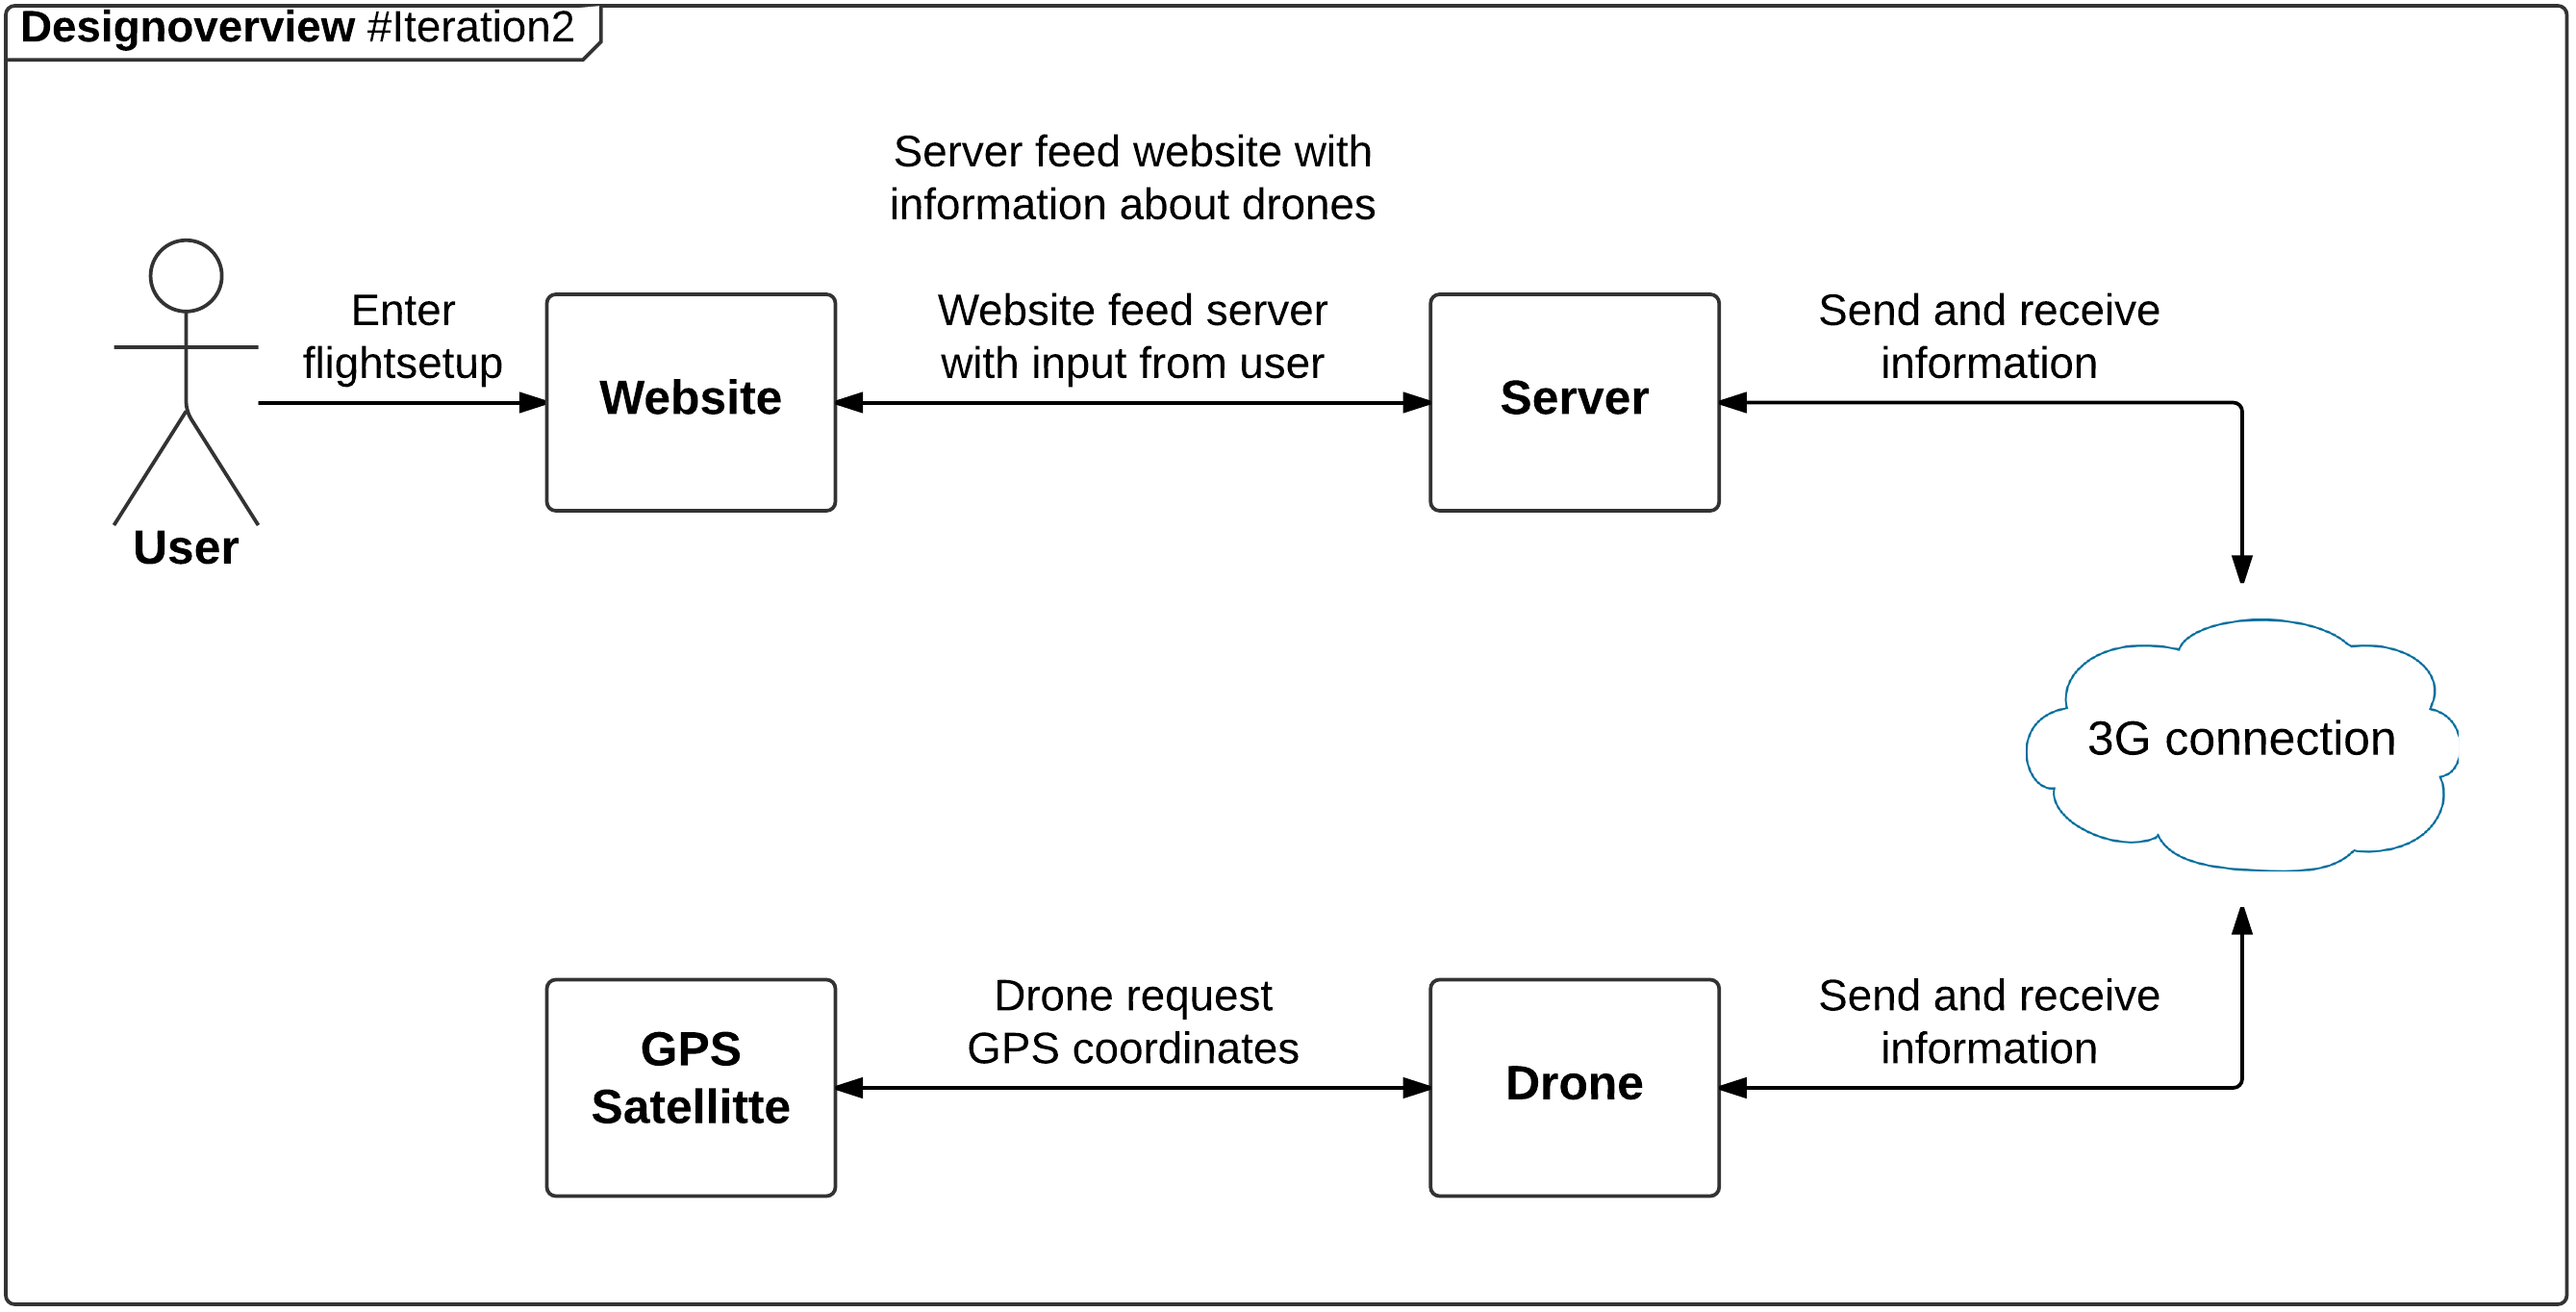
\includegraphics[width=1\textwidth]{Billeder/design_overview/design_overview_iteration2.png}
	\vspace{-.5cm}
	\caption{Designoverview \#iteration 2}
	\label{fig:design_overview_UC1}
\end{figure}


\newpage
\subsubsection*{Pakkediagram drone}
I dette afsnit vises pakkediagram tilhørende drone. De pakker der vises i pakkediagrammet består af en eller flere klasser, der med stort samspil udfører opgaver indenfor et fælles ansvarsområde. På hver pakke findes en lille beskrivelse, der tydeliggør pakkens ansvarsområde. De dele af pakkerne der er gråskraveret, er funktionalitet udarbejdet i tidligere iteration.


\begin{figure}[H]
	\centering
	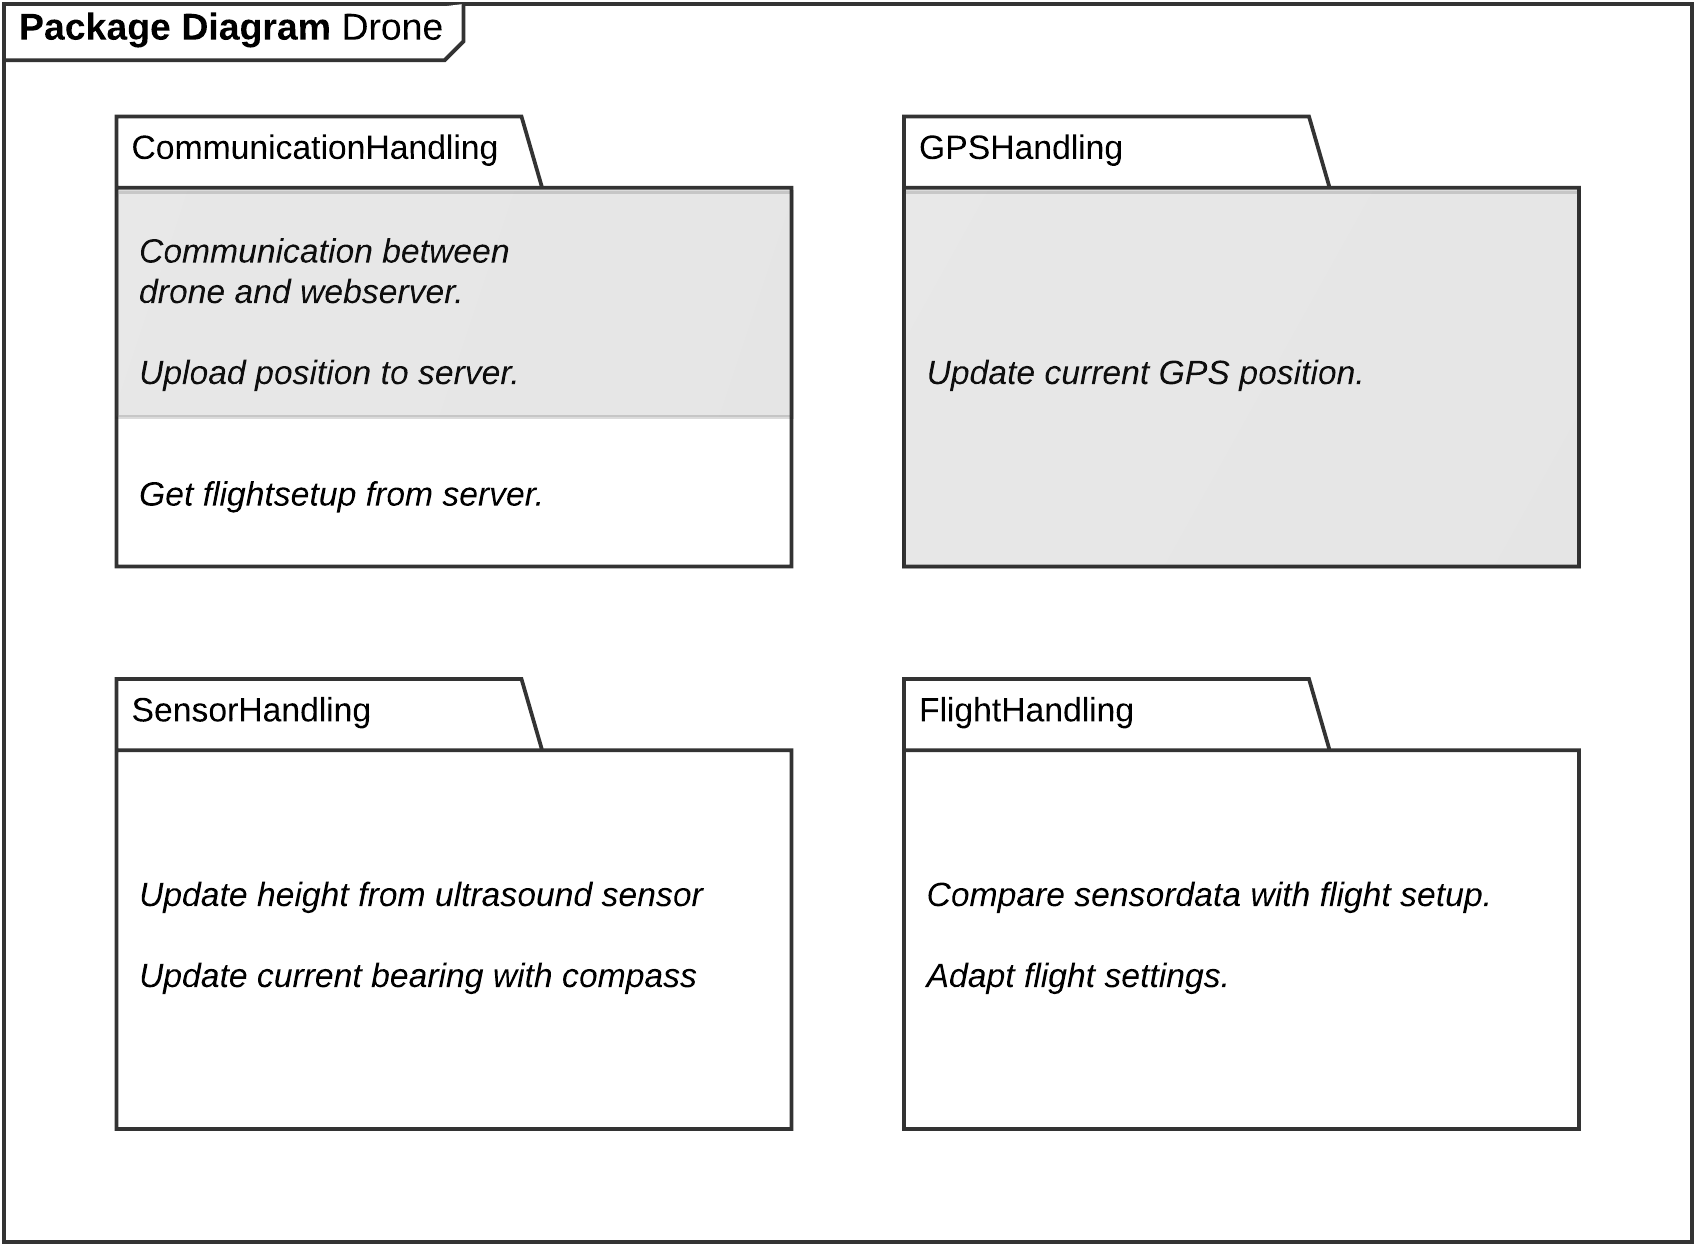
\includegraphics[width=1\textwidth]{Billeder/pakke_diagrammer/iteration2_drone.png}
	\vspace{-0.5cm}
	\caption{Pakkediagram drone}
	\label{fig:iteration2_pakke_diagram_drone}
\end{figure}

\textbf{CommunicationHandling}\\
Pakkens ansvar er kommunikation imellem drone og server. Efter denne iteration skal dronen både kunne hente flyveopsætninger fra server og sende sin nuværende GPS position til server.

\textbf{GPSHandling}\\
Pakkens ansvar er håndtering af GPS. Dels er pakken ansvarlig for opstart og initiering af GPS, og desuden bruges pakken hver gang dronens nuværende GPS position skal opdateres.

\textbf{SensorHandling}\\
Pakken er ansvarlig for indsamling af sensor data. I denne iteration skal pakken bruges til aflæsning af højdemåler og kompasset på flight control boardet. 

\textbf{FlightHandling}\\
Pakkens ansvar er kontrol og styring af drone under flyvning. Ved sammenligning af sensor data og data fra flyveopsætning tilpasses flyvehøjde, orientering mm



\newpage
\subsubsection*{Pakkediagram webapplikation}

I dette afsnit vises pakkediagram tilhørende webapplikation. De pakker der vises i pakkediagrammet består af en eller flere klasser, der med stort samspil udfører opgaver indenfor et fælles ansvarsområde. På hver pakke findes en lille beskrivelse, der tydeliggør pakkens ansvarsområde. De dele af pakkerne der er gråskraveret, er funktionalitet udarbejdet i tidligere iteration.

\begin{figure}[H]
	\centering
	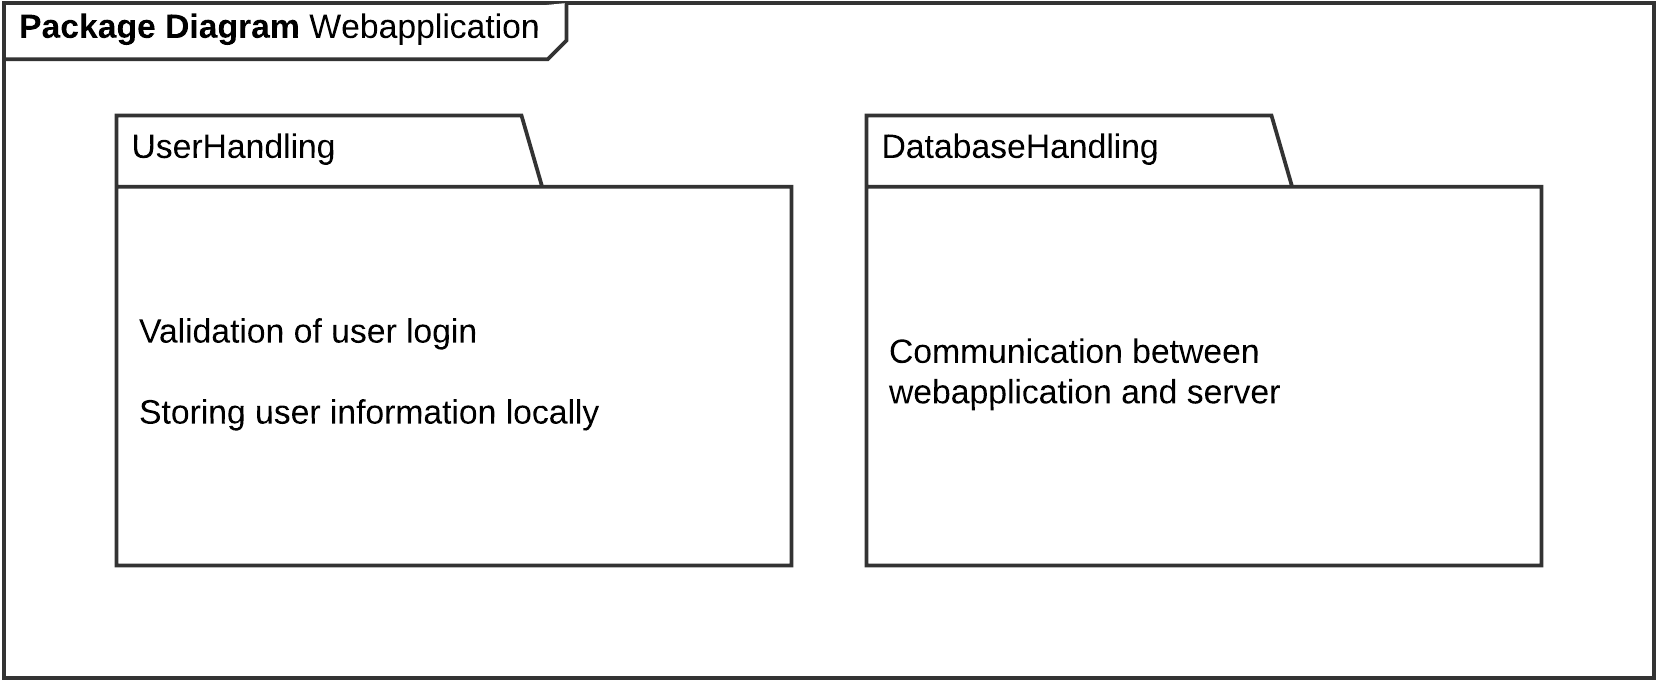
\includegraphics[width=1\textwidth]{Billeder/pakke_diagrammer/iteration1_server.png}
	\vspace{-0.5cm}
	\caption{Overordnet pakke diagram over webapplikationen}
	\label{fig:iteration1_pakke_diagram_webapp}
\end{figure}

\textbf{UserHandling}\\
Pakkens ansvar er validering af login/log ud på websitet. Pakken har også ansvaret for at hente og gemme data om den pågældende bruger.

\textbf{DatabaseHandling}\\
Pakkens ansvar er kommunikation imellem databasen og serveren. 

\textbf{DroneHandling}\\
Pakkens ansvar er alt data vedrørende dronen, så som håndteringen af events, waypoints og div droner.

\newpage

\subsubsection*{Sekvensdiagram drone}

Til iteration 2 er systemsekvensen beskrevet med 3 mindre sekvensdiagrammer i stedet for 1 stort. Ydermere er der lavet 2 sekvens diagrammer der går mere i dybden med 3G modulet og dens klasser. 
Denne fremstilling gør det muligt at repræsentere systemets funktionalitet på mere overskuelig vis, hvilket indirekte øger forståelsen af diagrammerne. Hvert af de 3 overordnede sekvensdiagrammer bruges til at fortælle hvordan en delmængde af systemet fungerer.

Af figur \ref{fig:Sekvens_diagram_iteration2_1} fremgår det hvordan bruger opretter en ny flyveopsætning. Det vises desuden hvilke interaktioner der foretages mellem bruger og website, samt hvordan server løbende indgår og benyttes i sekvensen. 

%kommentar
\begin{figure}[H]
	\centering
	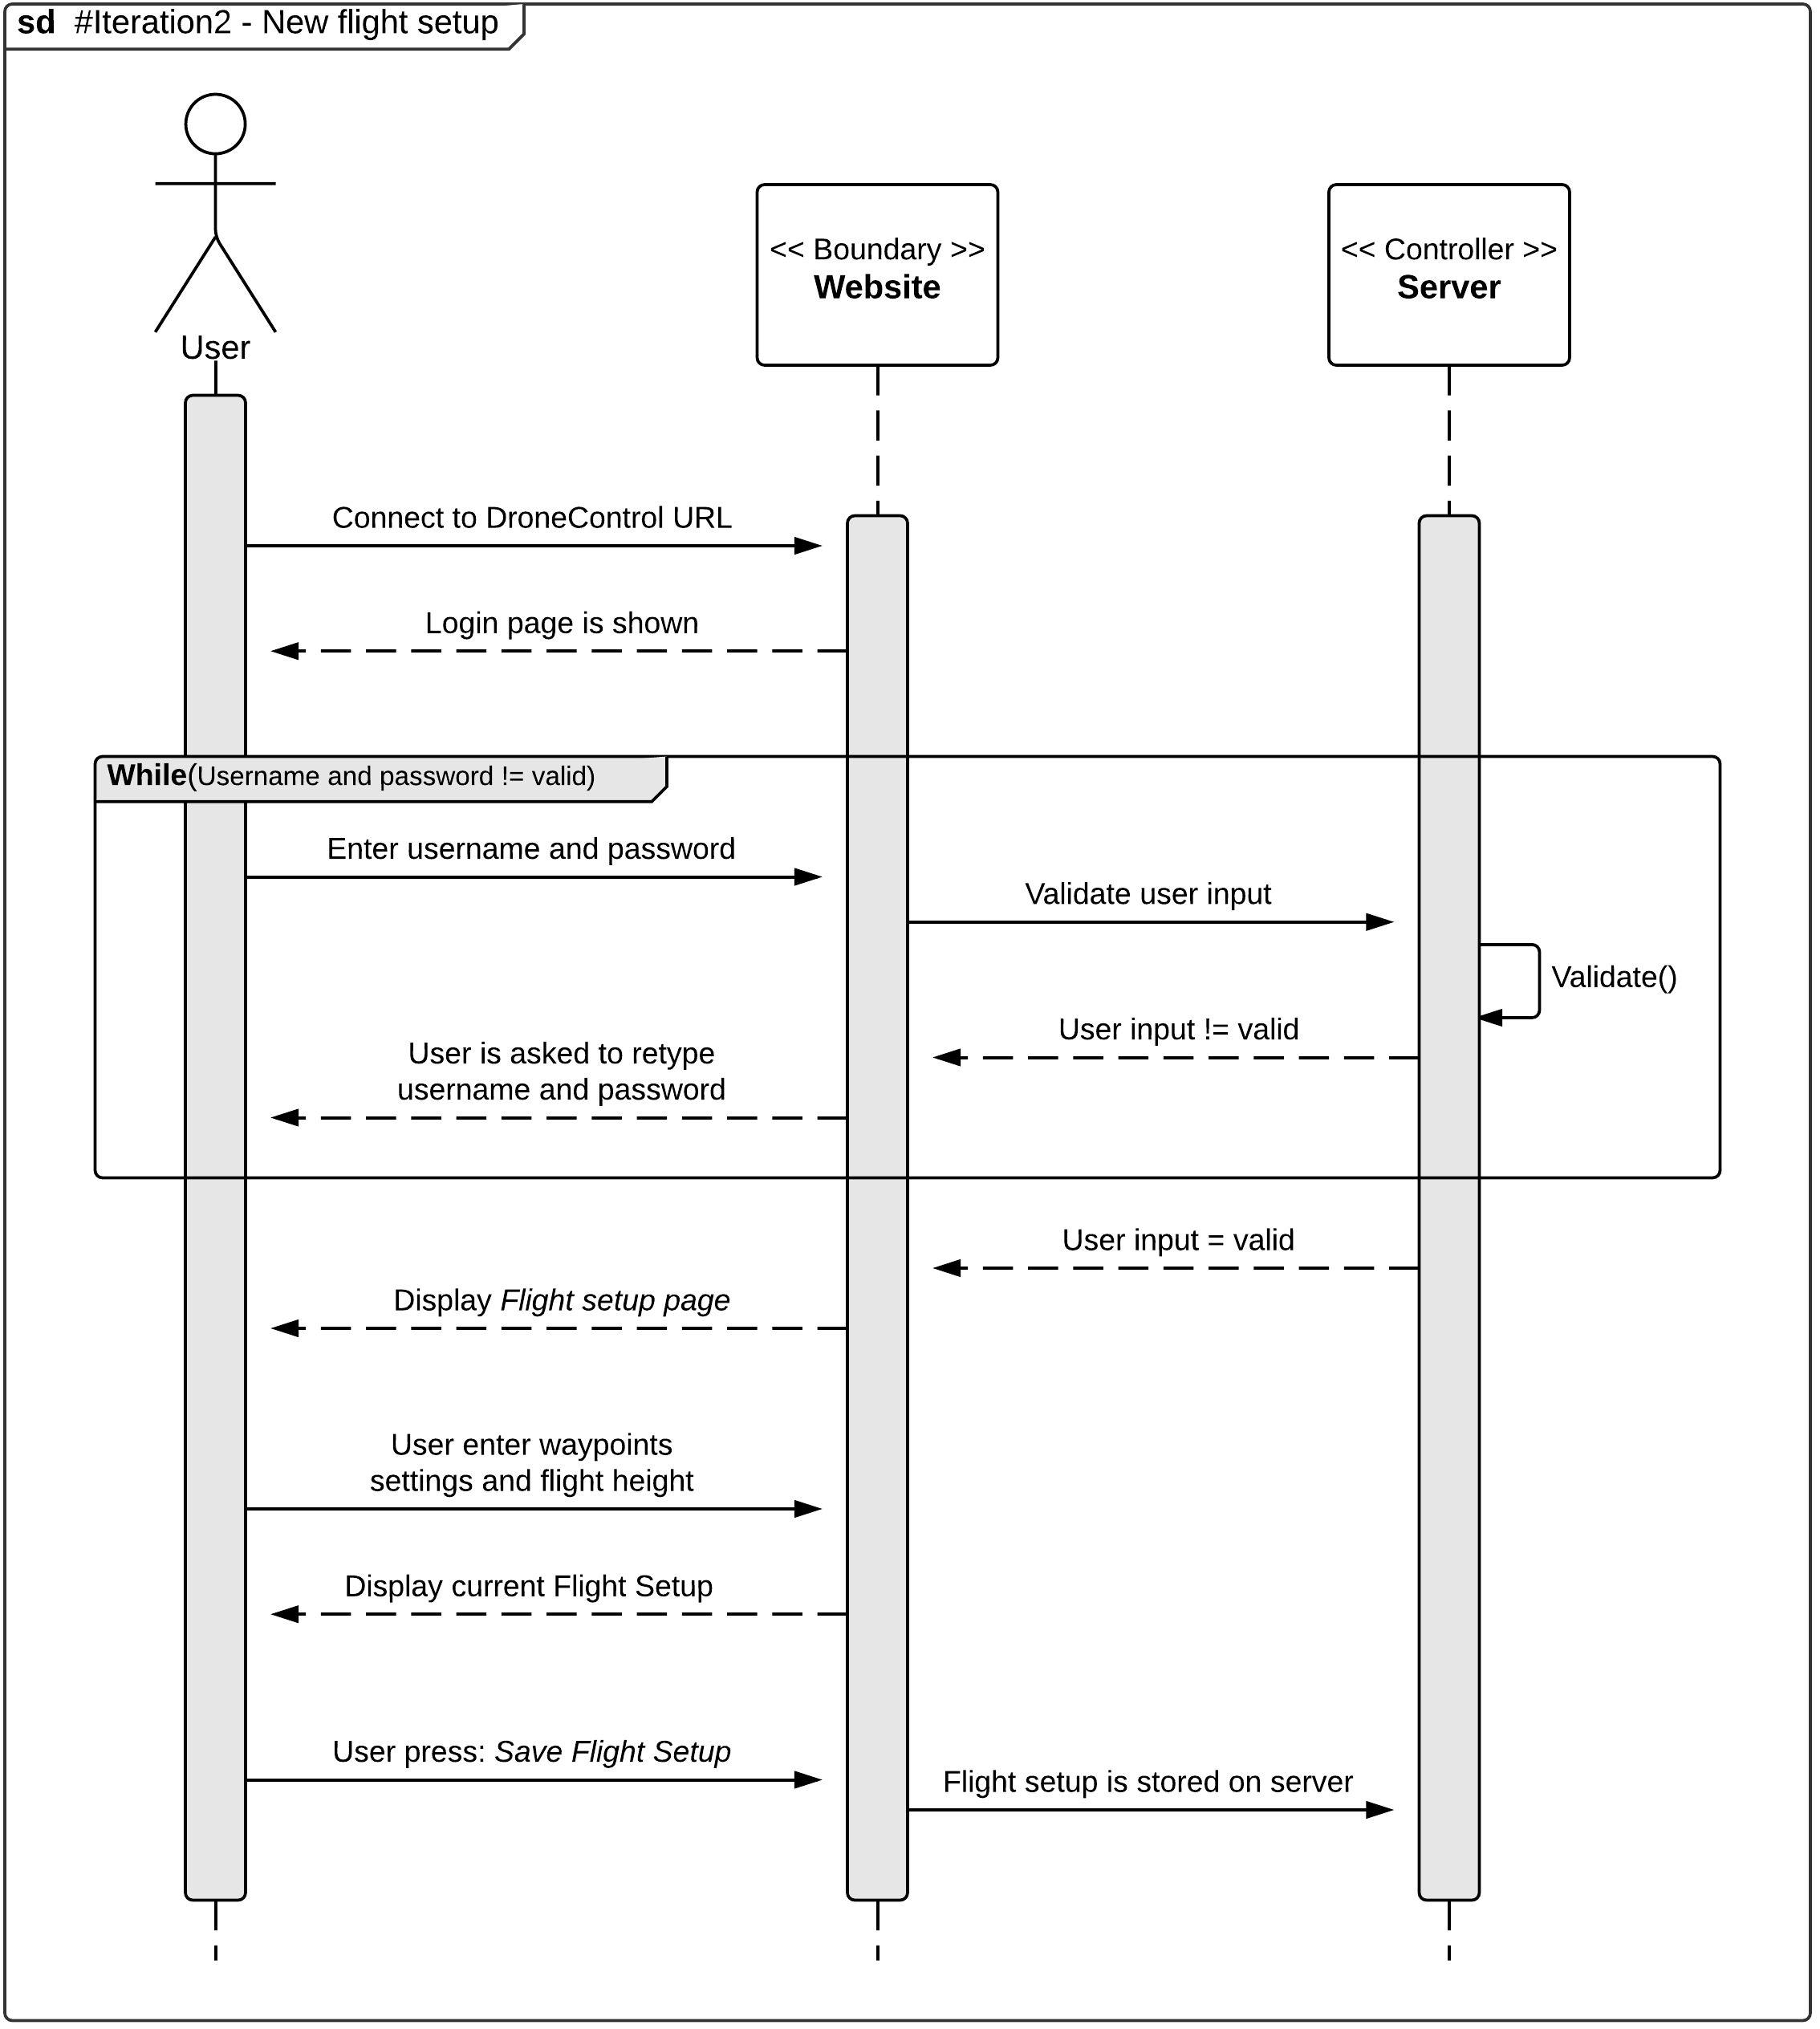
\includegraphics[width=1\textwidth]{Billeder/sekvens/sekvens_iteration2_1}
	\caption{Sekvensdiagram \#iteration 2}
	\label{fig:Sekvens_diagram_iteration2_1}
\end{figure}


\newpage

På figur \ref{fig:Sekvens_diagram_iteration2_2} fremgår det hvordan dronens main controller via 3G-shieldet kommunikerer med serveren for at kontrollere om der er en ny flyveopsætning tilgængelig. Det vises også hvilke beskeder der flyder frem og tilbage mellem main controller og server. Desuden vises det at dronen først henter ny flyveomsætning, når serveren har bekræftet, at der er en flyveopsætning tilgængelig.   

%kommentar
\begin{figure}[H]
	\centering
	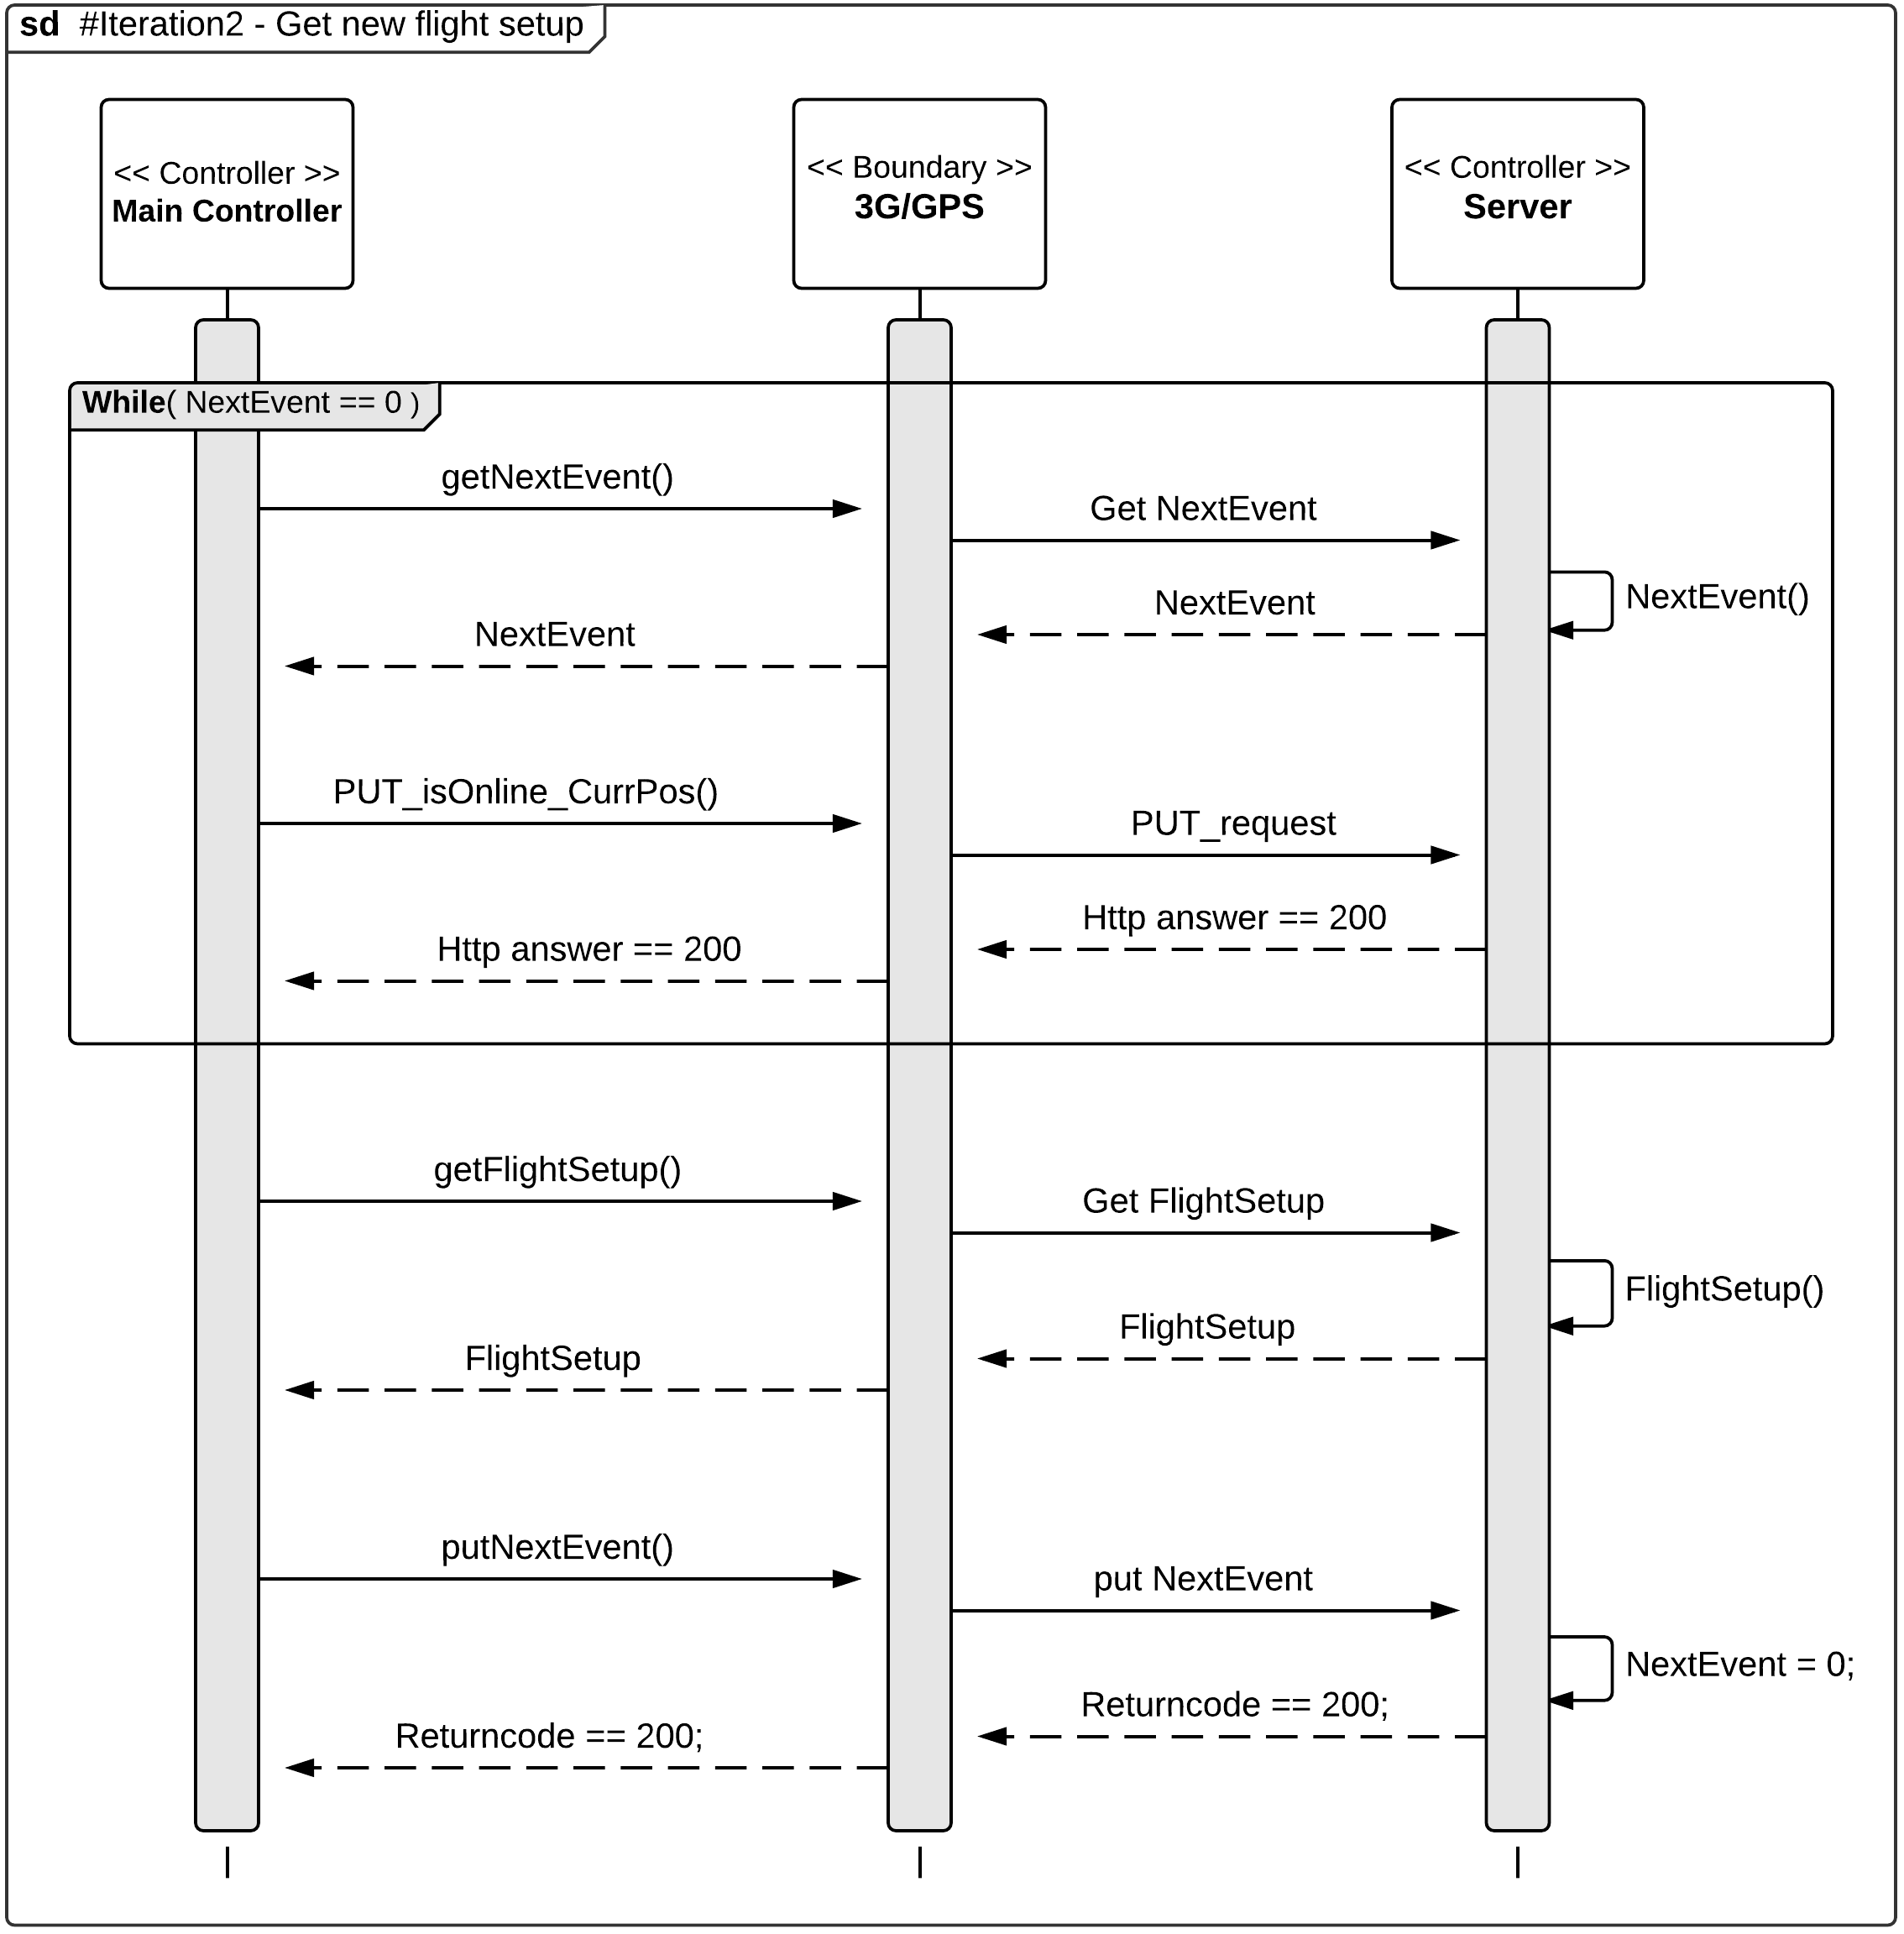
\includegraphics[width=1\textwidth]{Billeder/sekvens/sekvens_iteration2_2}
	\caption{Sekvensdiagram \#iteration 2}
	\label{fig:Sekvens_diagram_iteration2_2}
\end{figure}

\newpage

På Figur \ref{fig:Sekvens_getwaypoints} ses en mere detaljeret beskrivelse af 3G modulets klasser. Disse klasser håndterer al kommunikation mellem drone og server.

\begin{figure}[H]
	\centering
	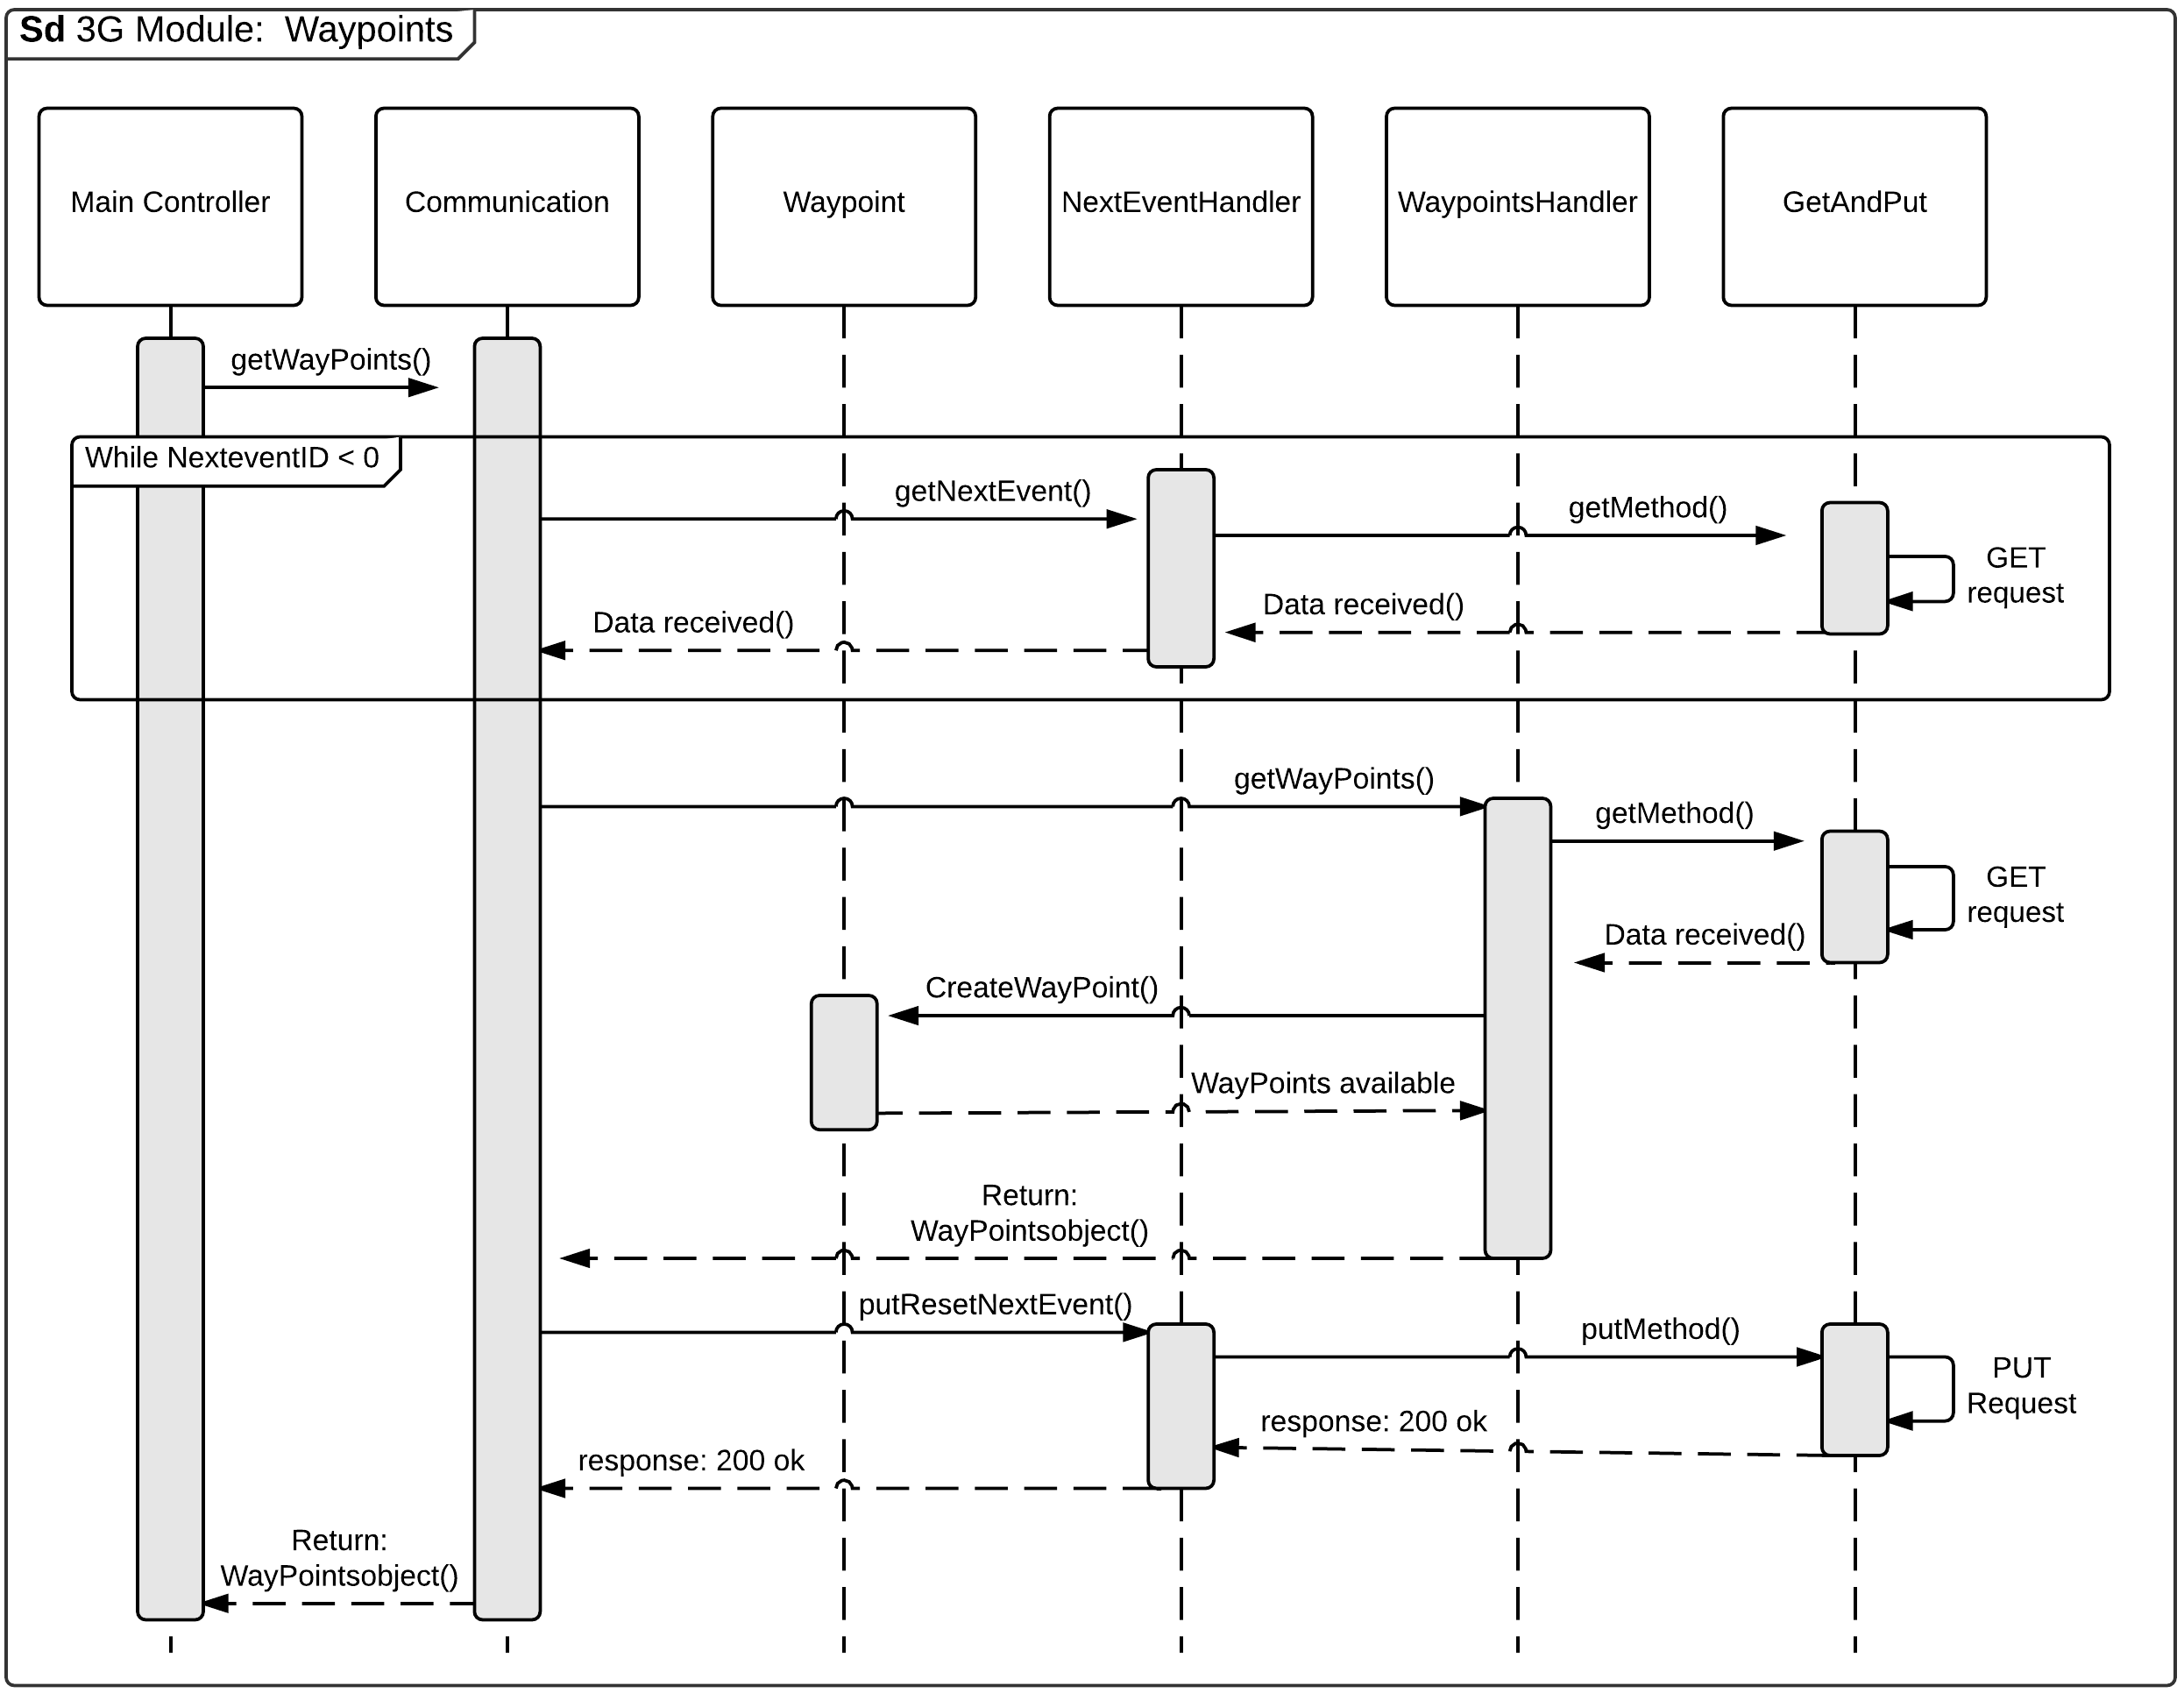
\includegraphics[width=1\textwidth]{Billeder/sekvens/sekvens_getwaypoints.png}
	\caption{Sekvensdiagram udvidet 3G module - getwaypoints}
	\label{fig:Sekvens_getwaypoints}
\end{figure}

\newpage

Af figur \ref{fig:Sekvens_diagram_iteration2_3} fremgår det hvordan dronen opererer når den flyver autonomt mod en givet GPS position. Main controlleren indsamler kompas data fra flight control boardet, latitude og longitude fra 3G/GPS modulet og flyvehøjde fra ultralyds sensoren. Den indhentede data processeres og bruges til at korrigerer de nuværende flyveindstillinger.
Som det fremgår af while loopet fortsætter flyvningen indtil dronen er 15 meter fra den GPS destination bruger valgte i flyveopsætningen. 


%kommentar
\begin{figure}[H]
	\centering
	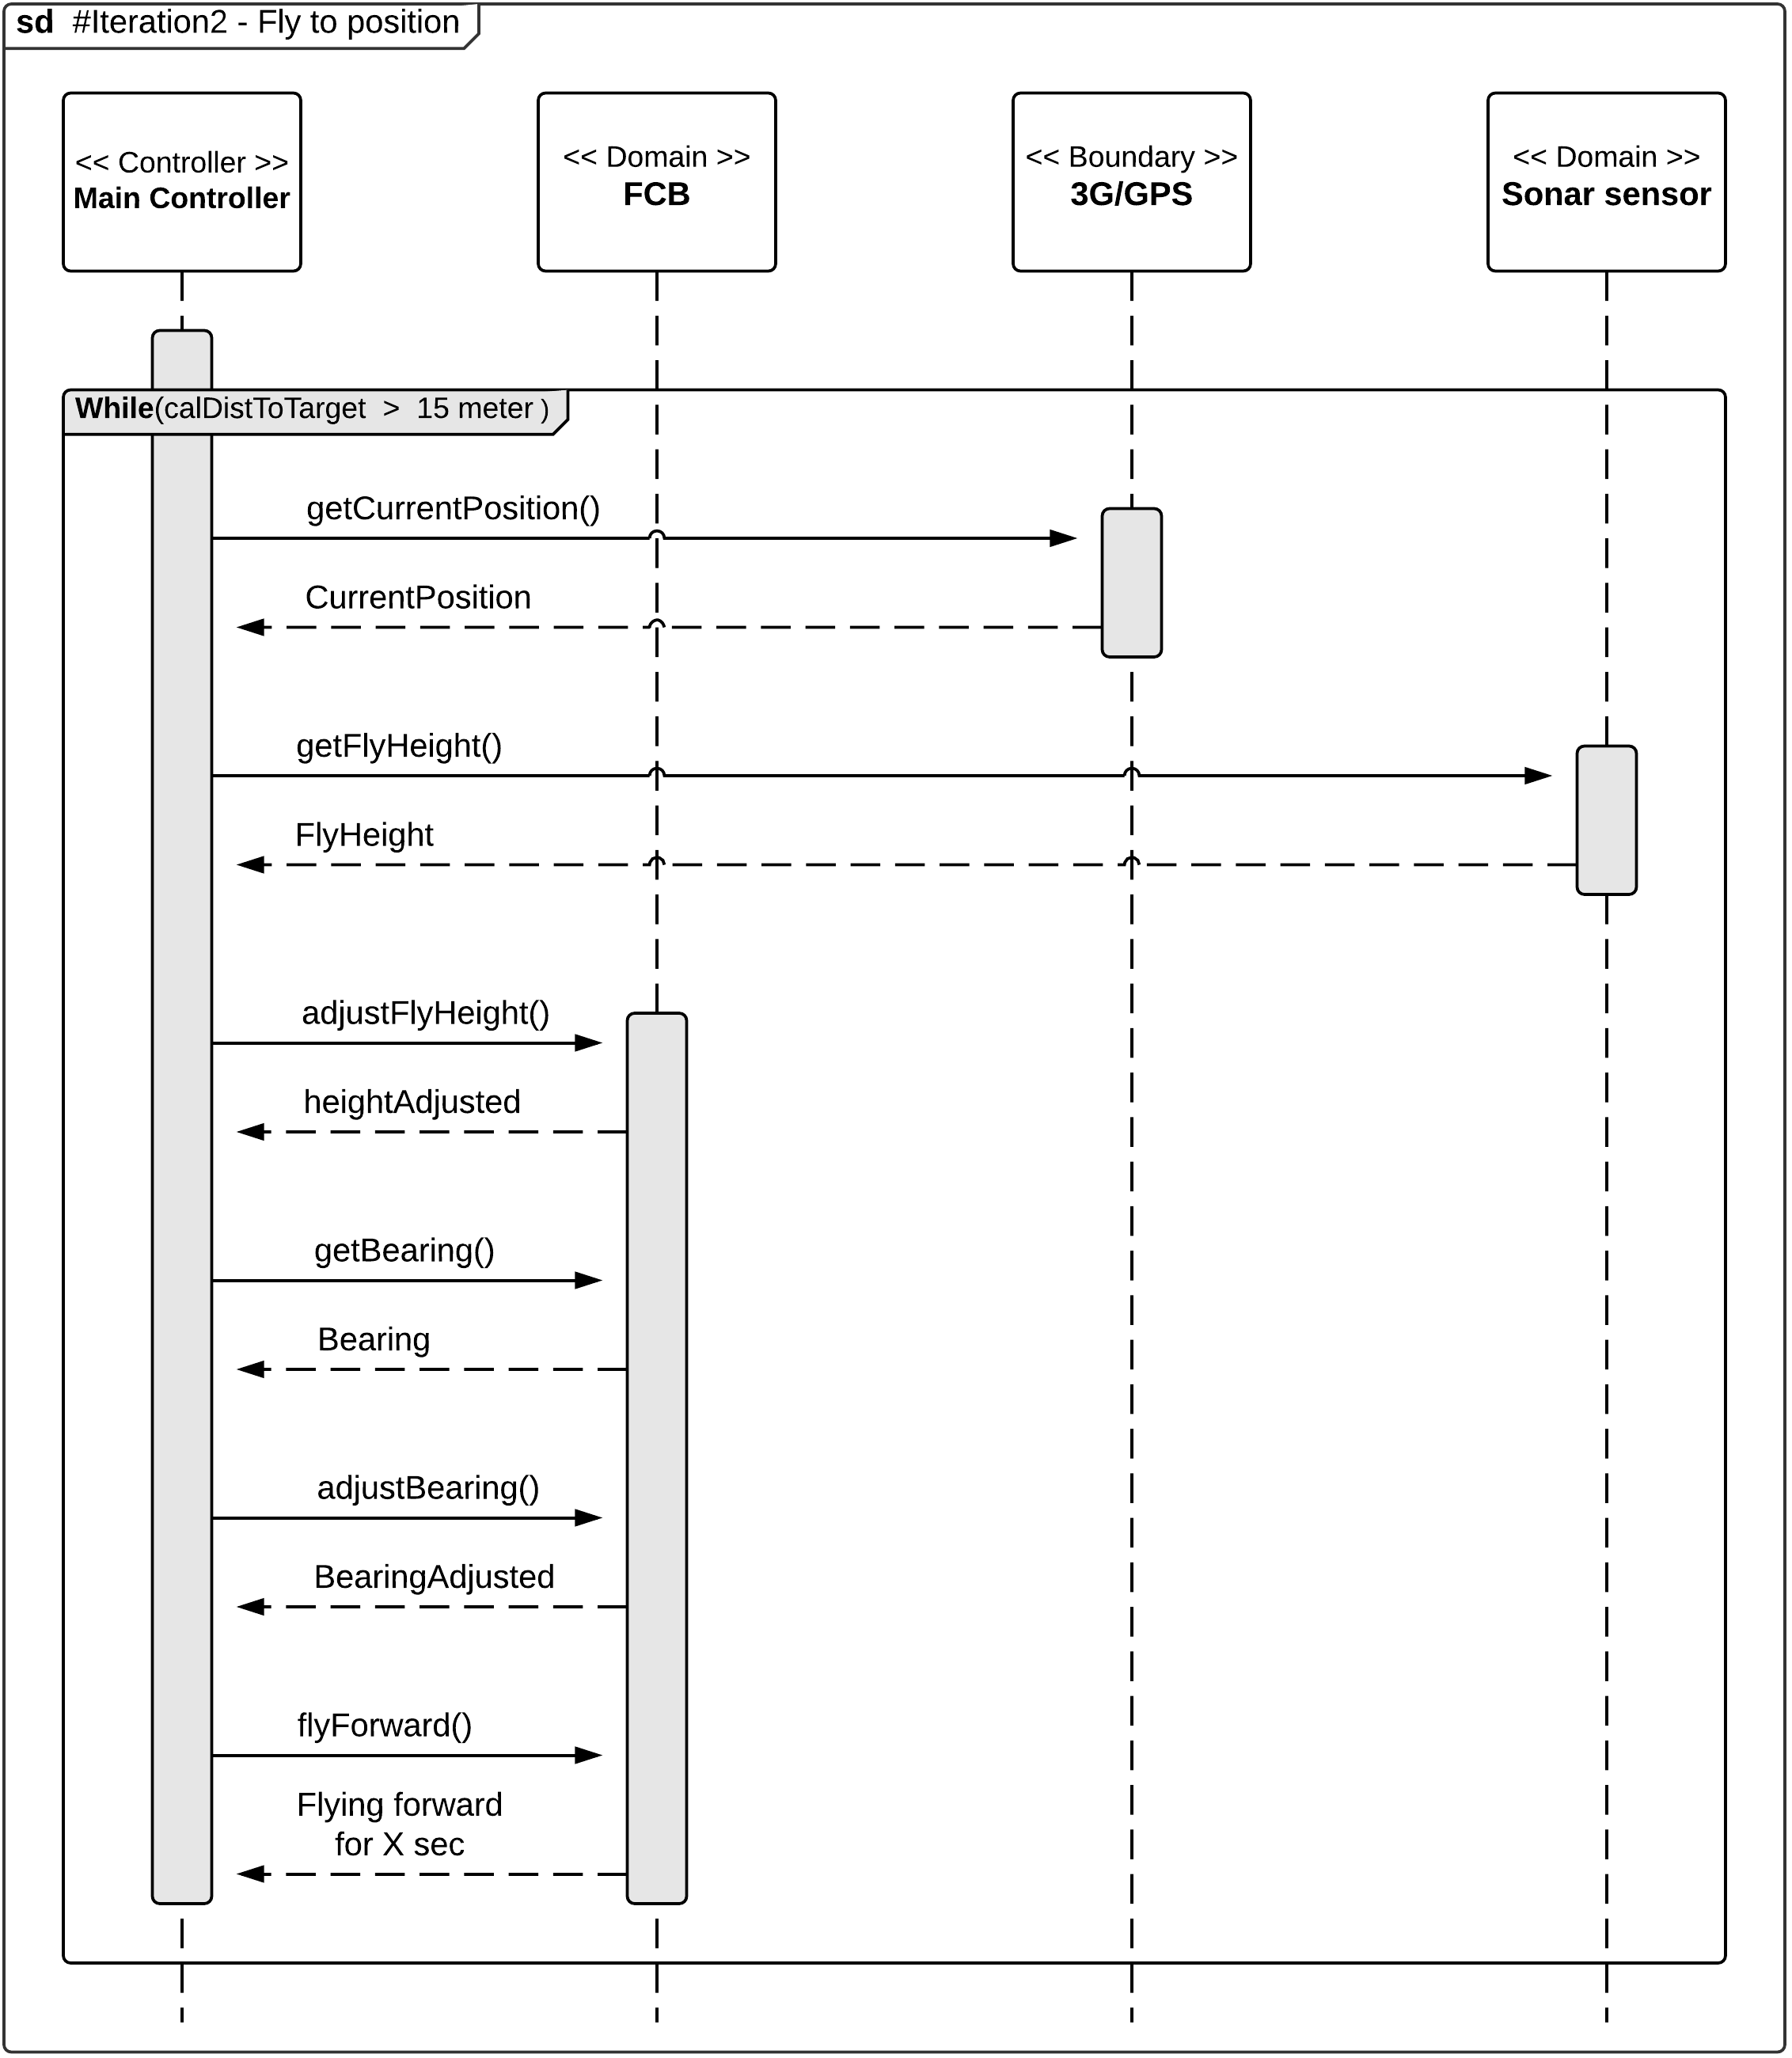
\includegraphics[width=1\textwidth]{Billeder/sekvens/sekvens_iteration2_3}
	\caption{Sekvensdiagram \#iteration 2}
	\label{fig:Sekvens_diagram_iteration2_3}
\end{figure}

\newpage
\subsubsection*{Sekvensdiagram webapplikation}
\vspace{-0.1cm}
På figur \ref{fig:page_load} ses hvordan klasserne på websitet interagere med hinanden ved et page load. Kortet bliver initialiseret med centrum over århus og drone markeren bliver initialiseret. Useren som blev gemt ved login bliver brugt til at give en velkomst besked oppe i højre hjørne og sener vil blive brugt når der skal oprettet nye events. Listen med tilgængelige droner bliver loaded. Et click event bliver også oprettet som trigger ved click på kortet til oprettelse af nye waypoints.
\begin{figure}[H]
	\centering
	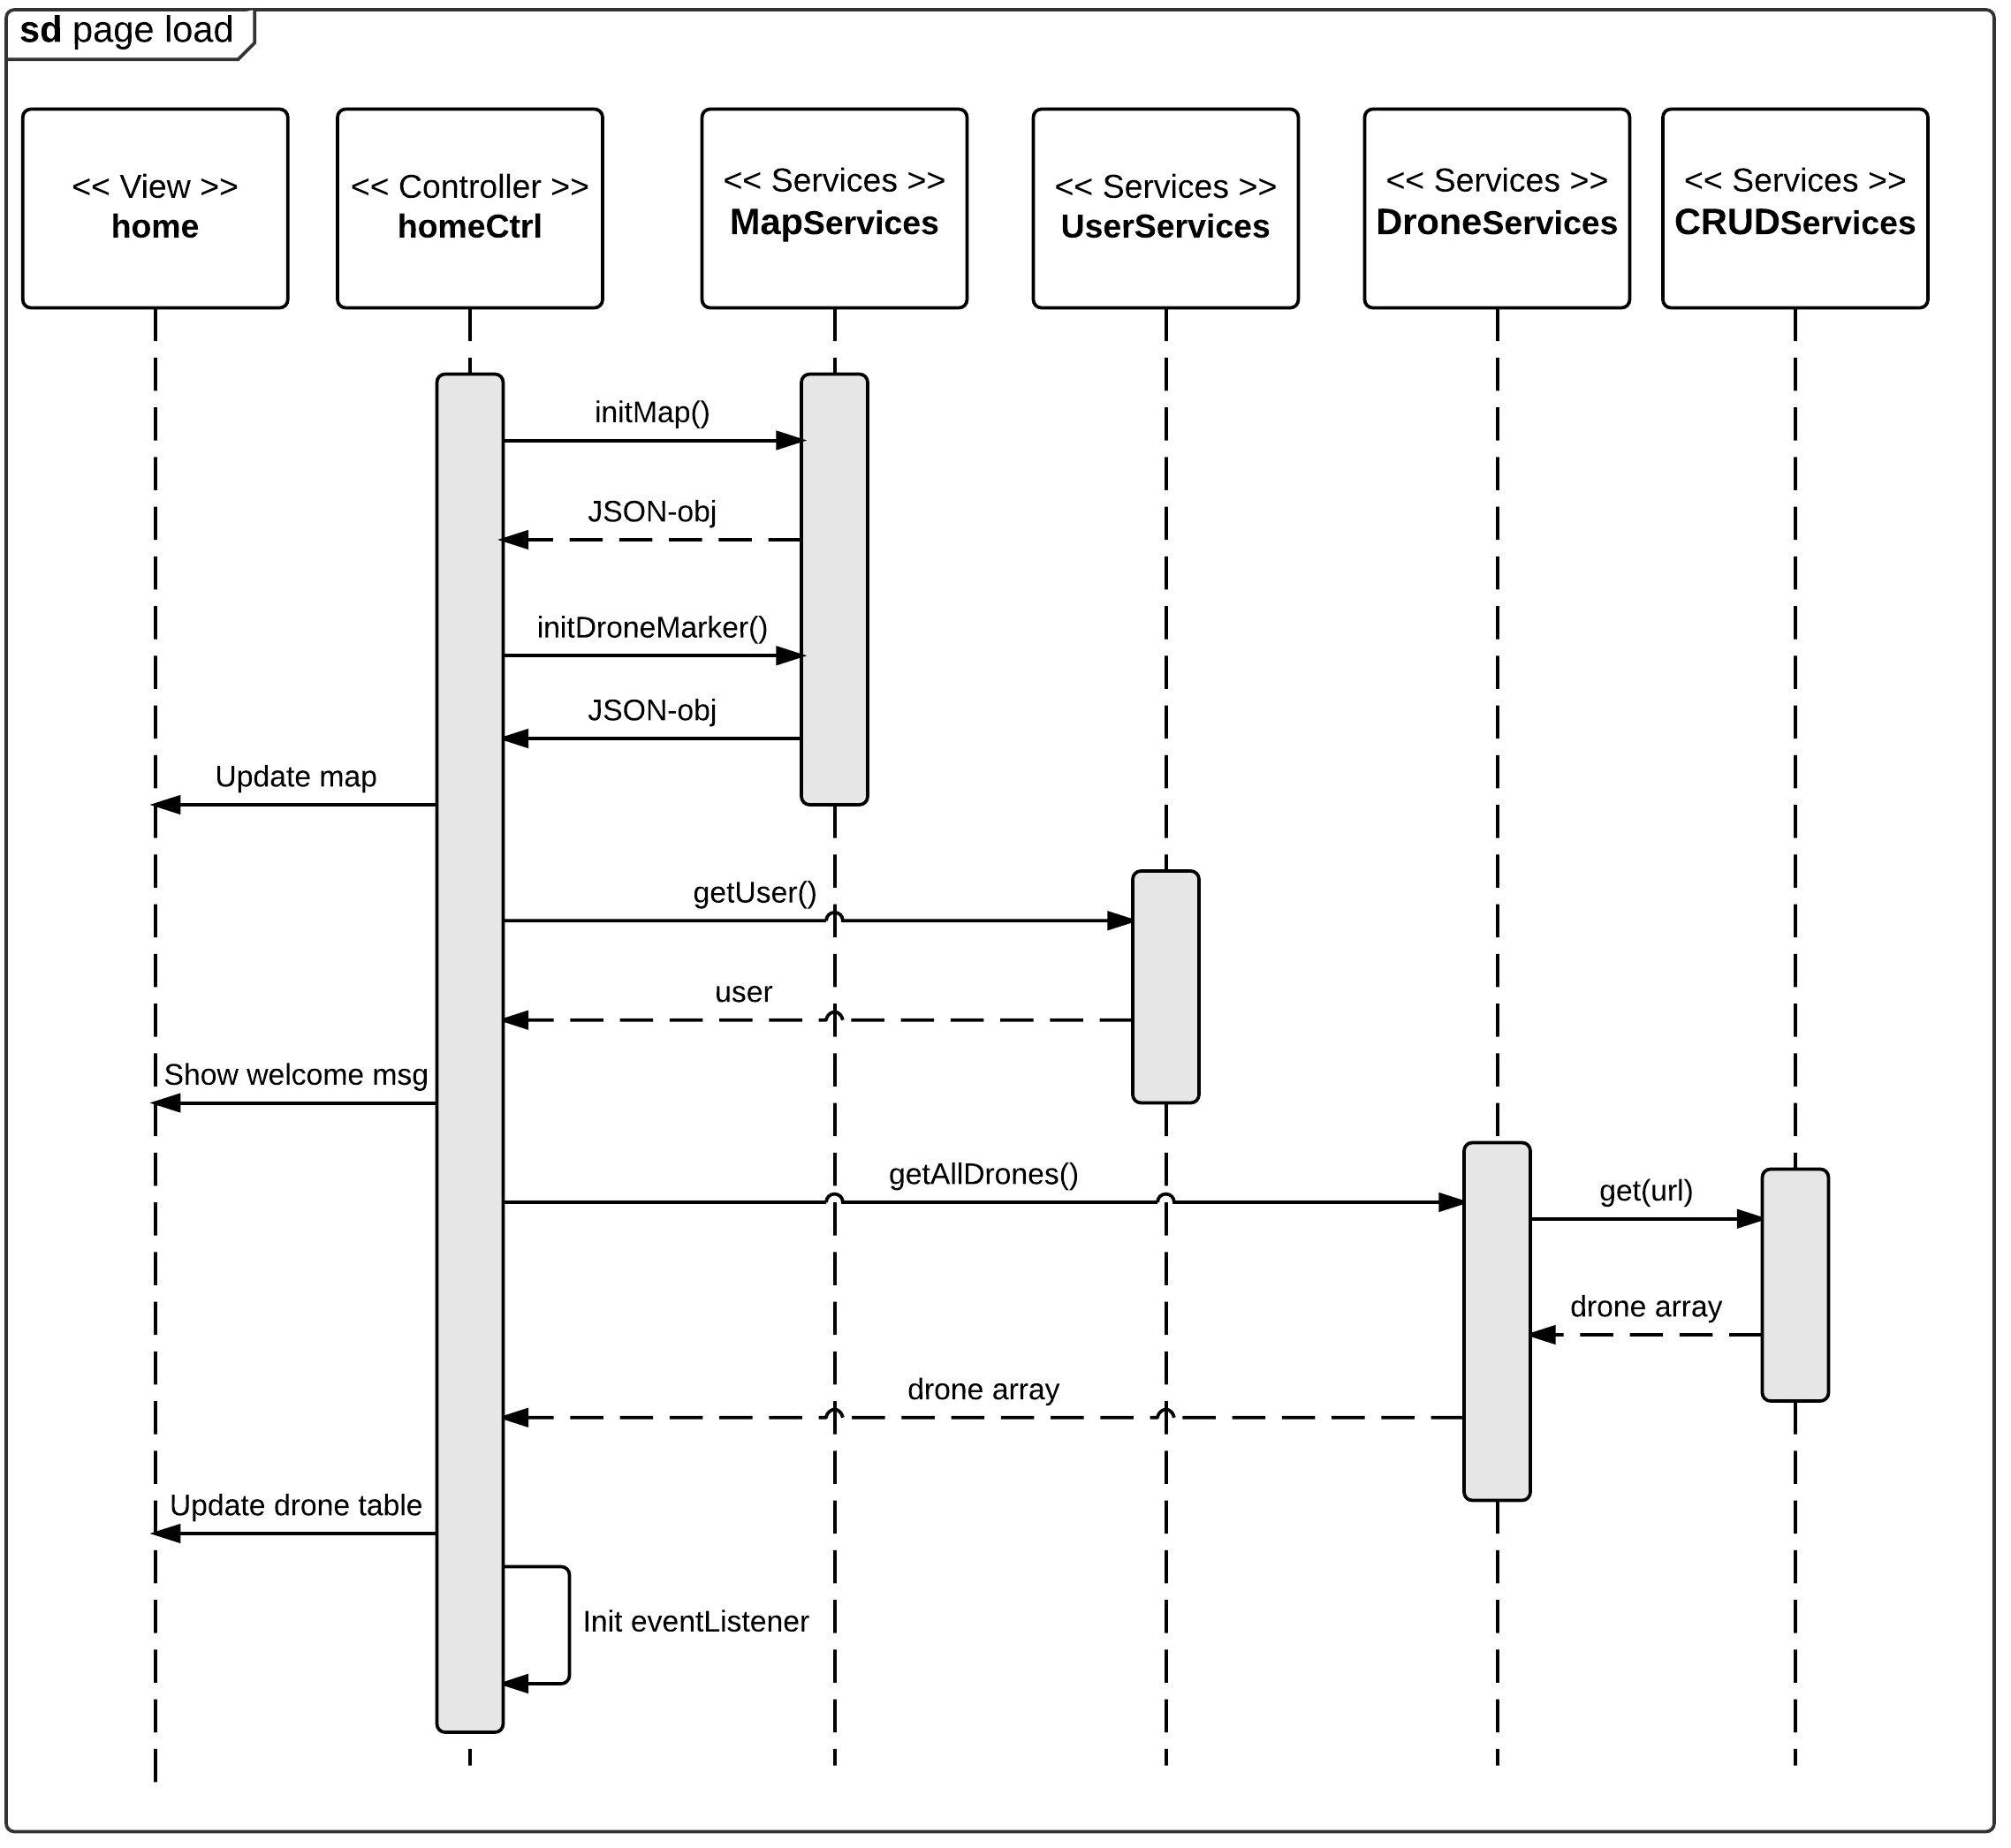
\includegraphics[width=1\textwidth]{Billeder/sekvens/sd_page_load.png}
	\caption{Sekvensdiagram page load}
	\label{fig:page_load}
\end{figure}

\newpage
På figur \ref{fig:send_waypoints} ses hvilke hændelser der finder sted i systemet, når useren trykker på "send event". Hvert services har et ansvar og det er dem der kommunikere ud til CRUD-servicesen, på den måde er logikken for data håndtering skubbet ud i div. services. 
\begin{figure}[H]
	\centering
	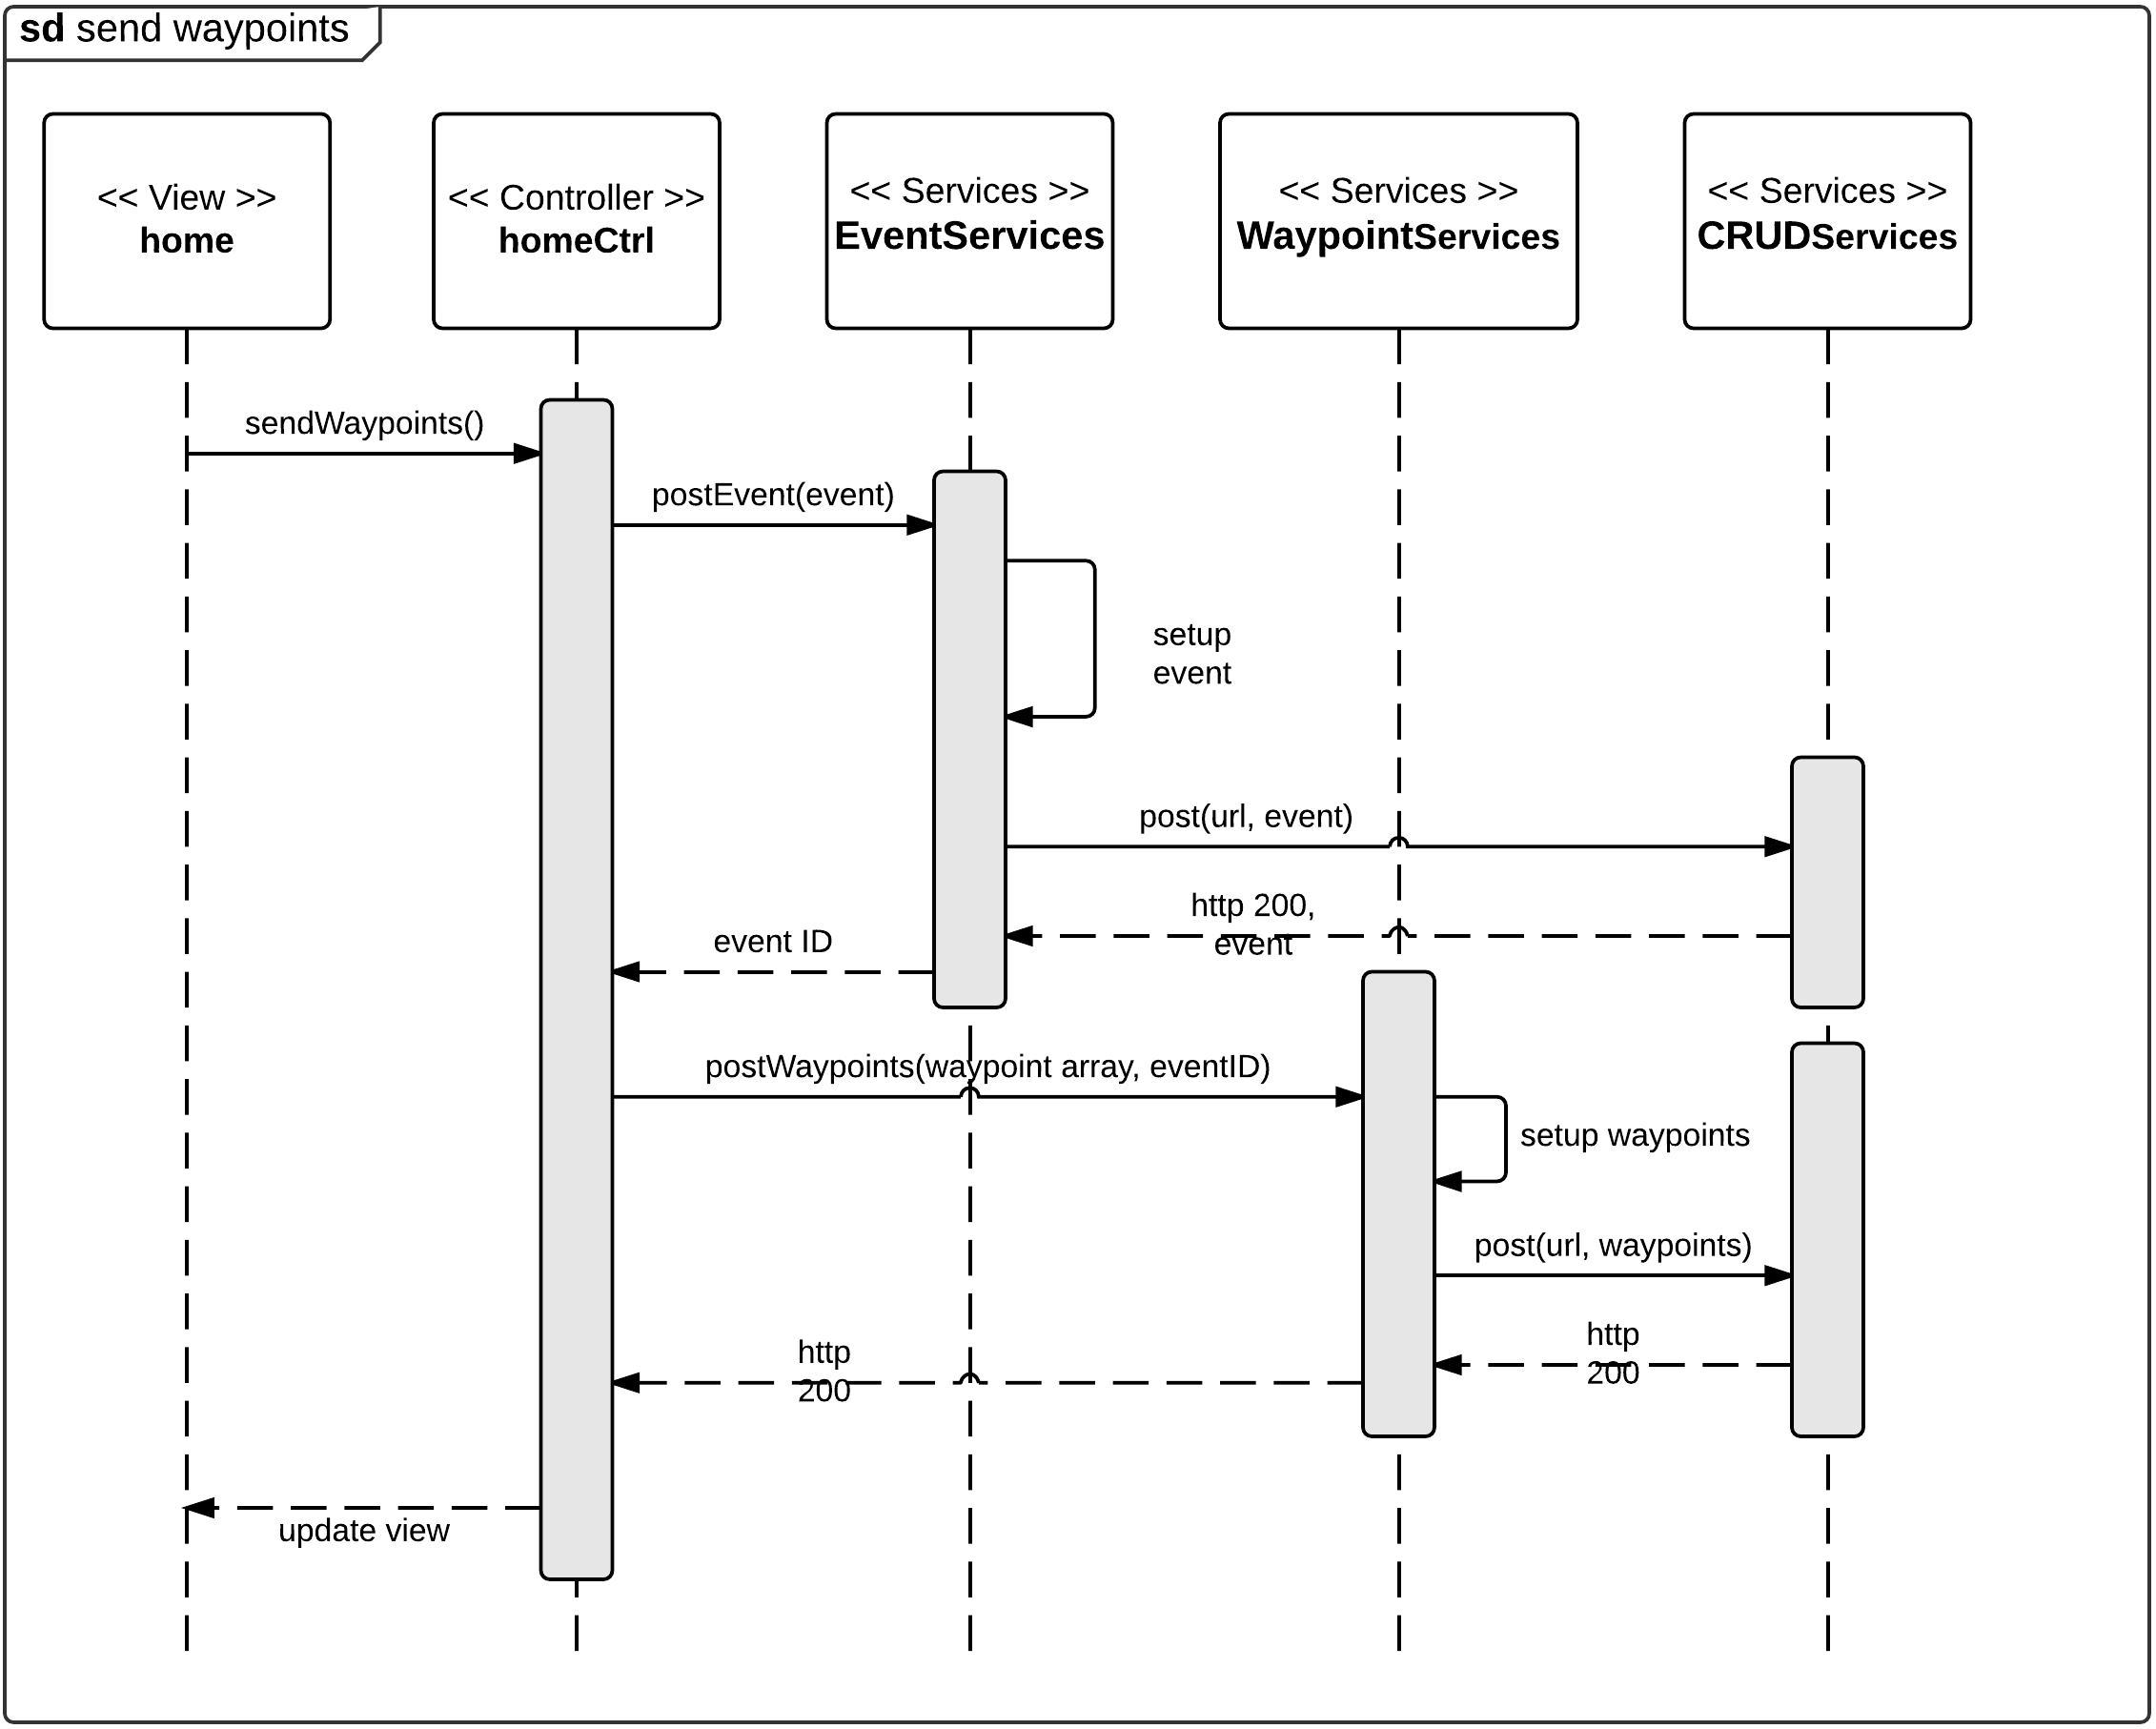
\includegraphics[width=1\textwidth]{Billeder/sekvens/sd_send_waypoints.png}
	\caption{Sekvensdiagram send waypoints}
	\label{fig:send_waypoints}
\end{figure}

\newpage
På figur \ref{fig:update_view} ses hvilke hændelser der finder sted i systemet, når useren trykker på forskellige droner i tabellen. Når et klik på tabellen finder sted skal view'et opdateret i forhold til den givet drone, dvs. hvis dronen har et event, så skal det vises og dertilhørende waypoints. Hvis der ikke er noget event tilknyttet til dronen skal useren have mulighed for at oprette et nyt event.
\begin{figure}[H]
	\centering
	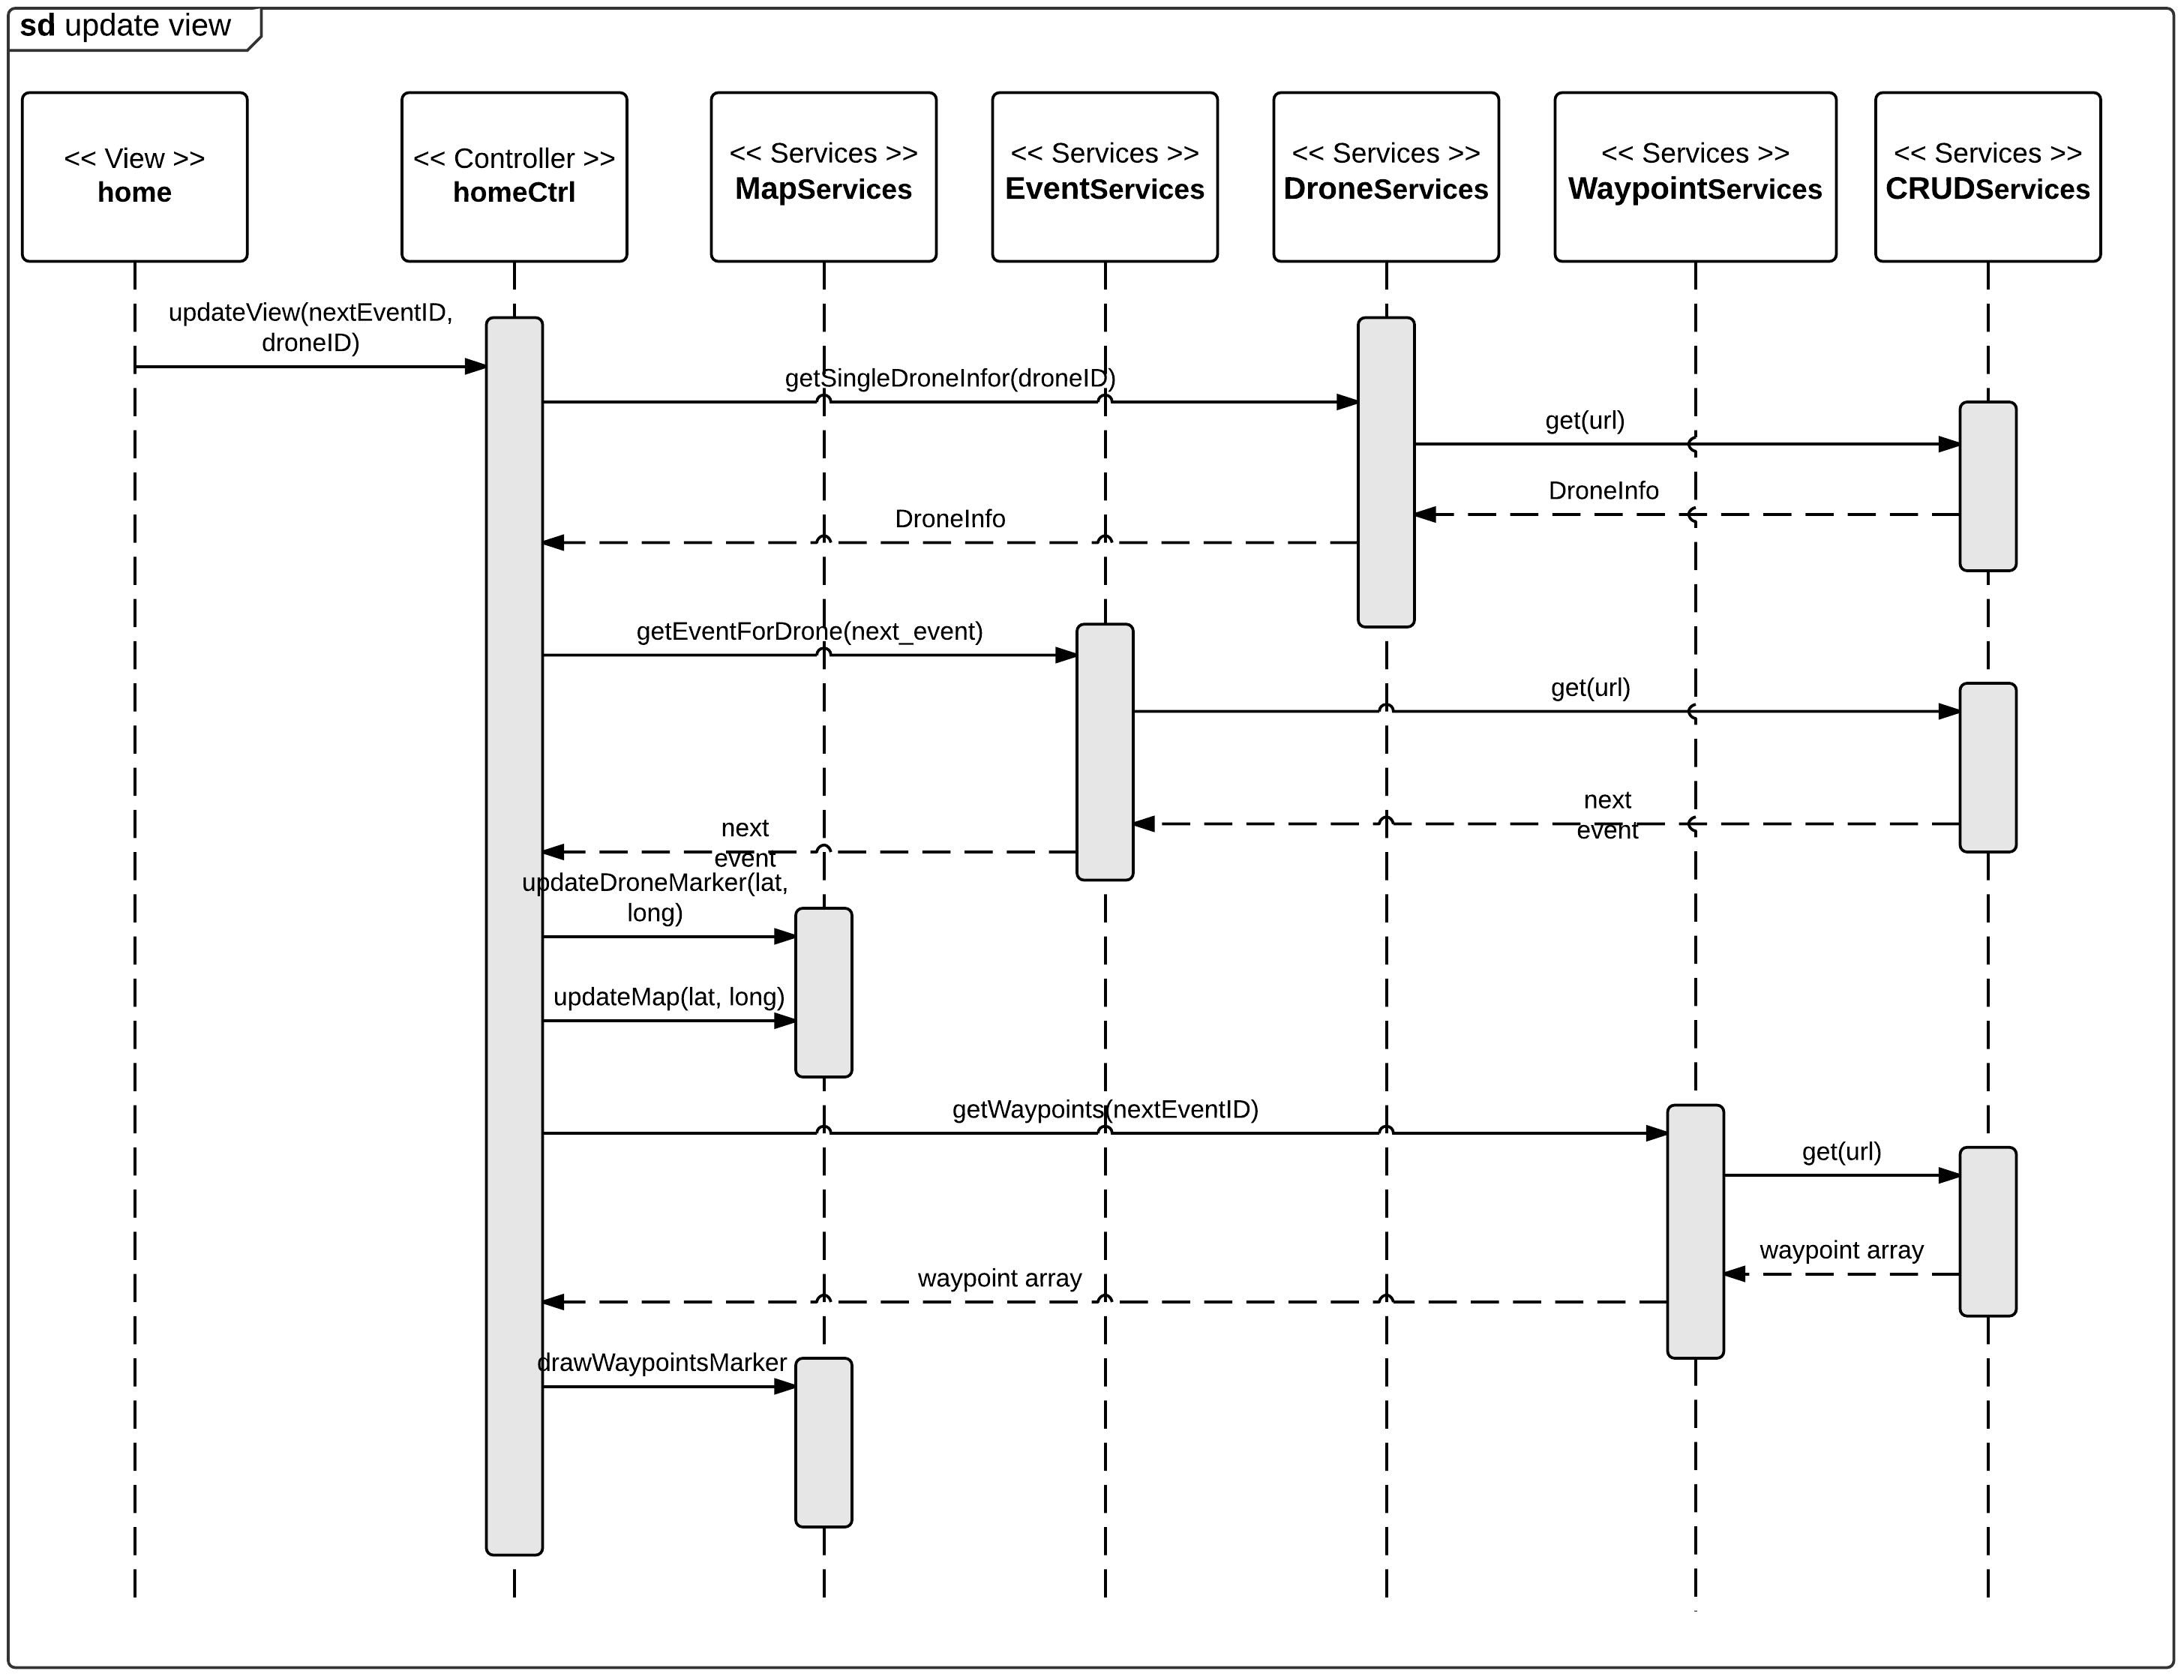
\includegraphics[width=1\textwidth]{Billeder/sekvens/sd_update_view.png}
	\caption{Sekvensdiagram opdater }
	\label{fig:update_view}
\end{figure}

\newpage
\subsubsection*{Klassediagram drone}

På figur \ref{fig:classDiagram_drone_underflyvning} ses klasse diagrammet for dronen. Det er klasserne der bruges af dronen, når den er flyve klar. På den følgende side er der en forklaring af klasserne og deres metoder. 

\begin{figure}[H]
	\centering
	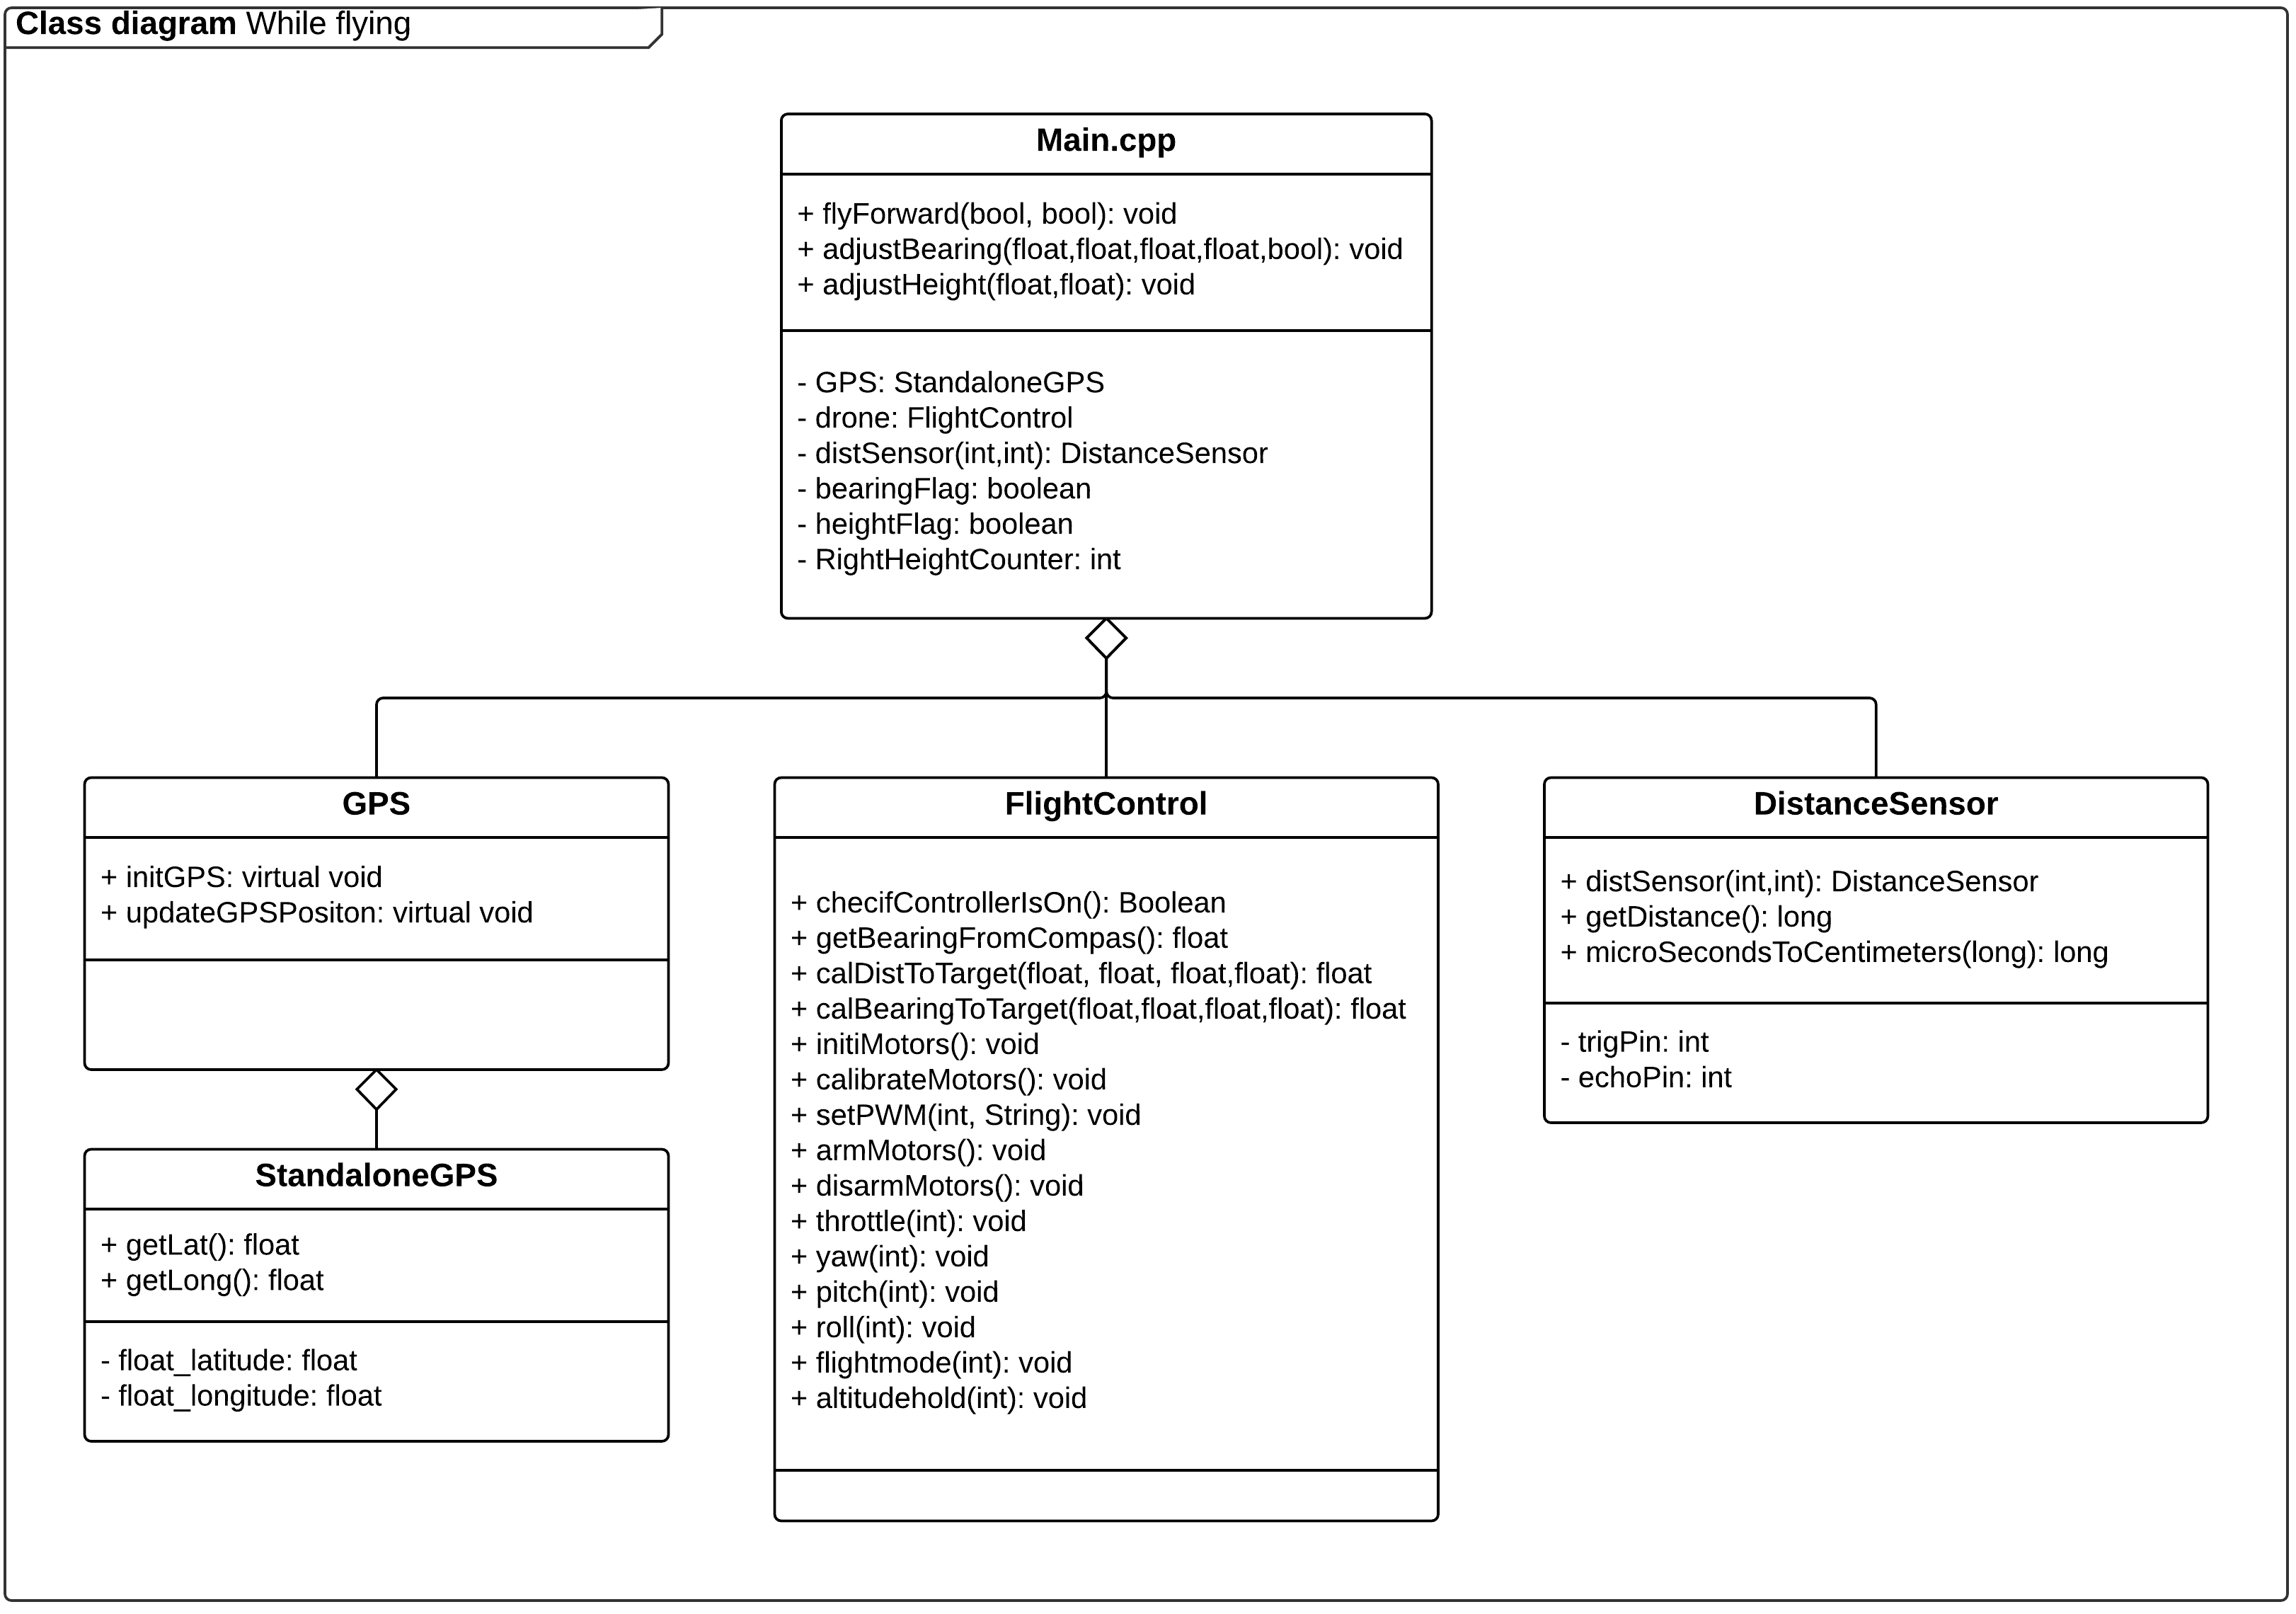
\includegraphics[width=1\textwidth]{Billeder/klasse_diagrammer/classdiagram_iteration2_fly.png}
	\vspace{0cm}
	\caption{Klassediagram drone}
	\label{fig:classDiagram_drone_underflyvning}
\end{figure}

\textbf{FlightControl} \\
Det er Flight Control klassen der har alt med styring af dronen at gøre, lige fra calibrering af motorerne til at hente data fra kompasset. 

\textbf{DistanceSensor} \\
DistanceSensor klassen bruges til at kontrollere de sensorer der er monteret på dronen. Her er det både sensorer til højdemåling og anti kollision. 

\textbf{GPS} \\
GPS klassen er implementeret som en abstract klasse, idet den ikke selv har nogle metoder den skal bruge, men med virtuelle metoder der sikrer at de implementeres i de afledte klasser. 
Init og updateGPSPosition er valgt til at være virtuelle klasser, hvilket gør at de skal implementeres uanset hvilken GPS der bruges. Klassen er lavet fordi der i udgangspunkt var mulighed for at bruge 3 forskellige slags GPS modes med 3G/GPS shieldet. 

\newpage
På Figur \ref{fig:classDiagram_3Gmodul} er der vist en udvidet klasse diagram for 3G modulet. På diagrammet vises de metoder og attributter der indgår i klasserne. 

\begin{figure}[H]
	\centering
	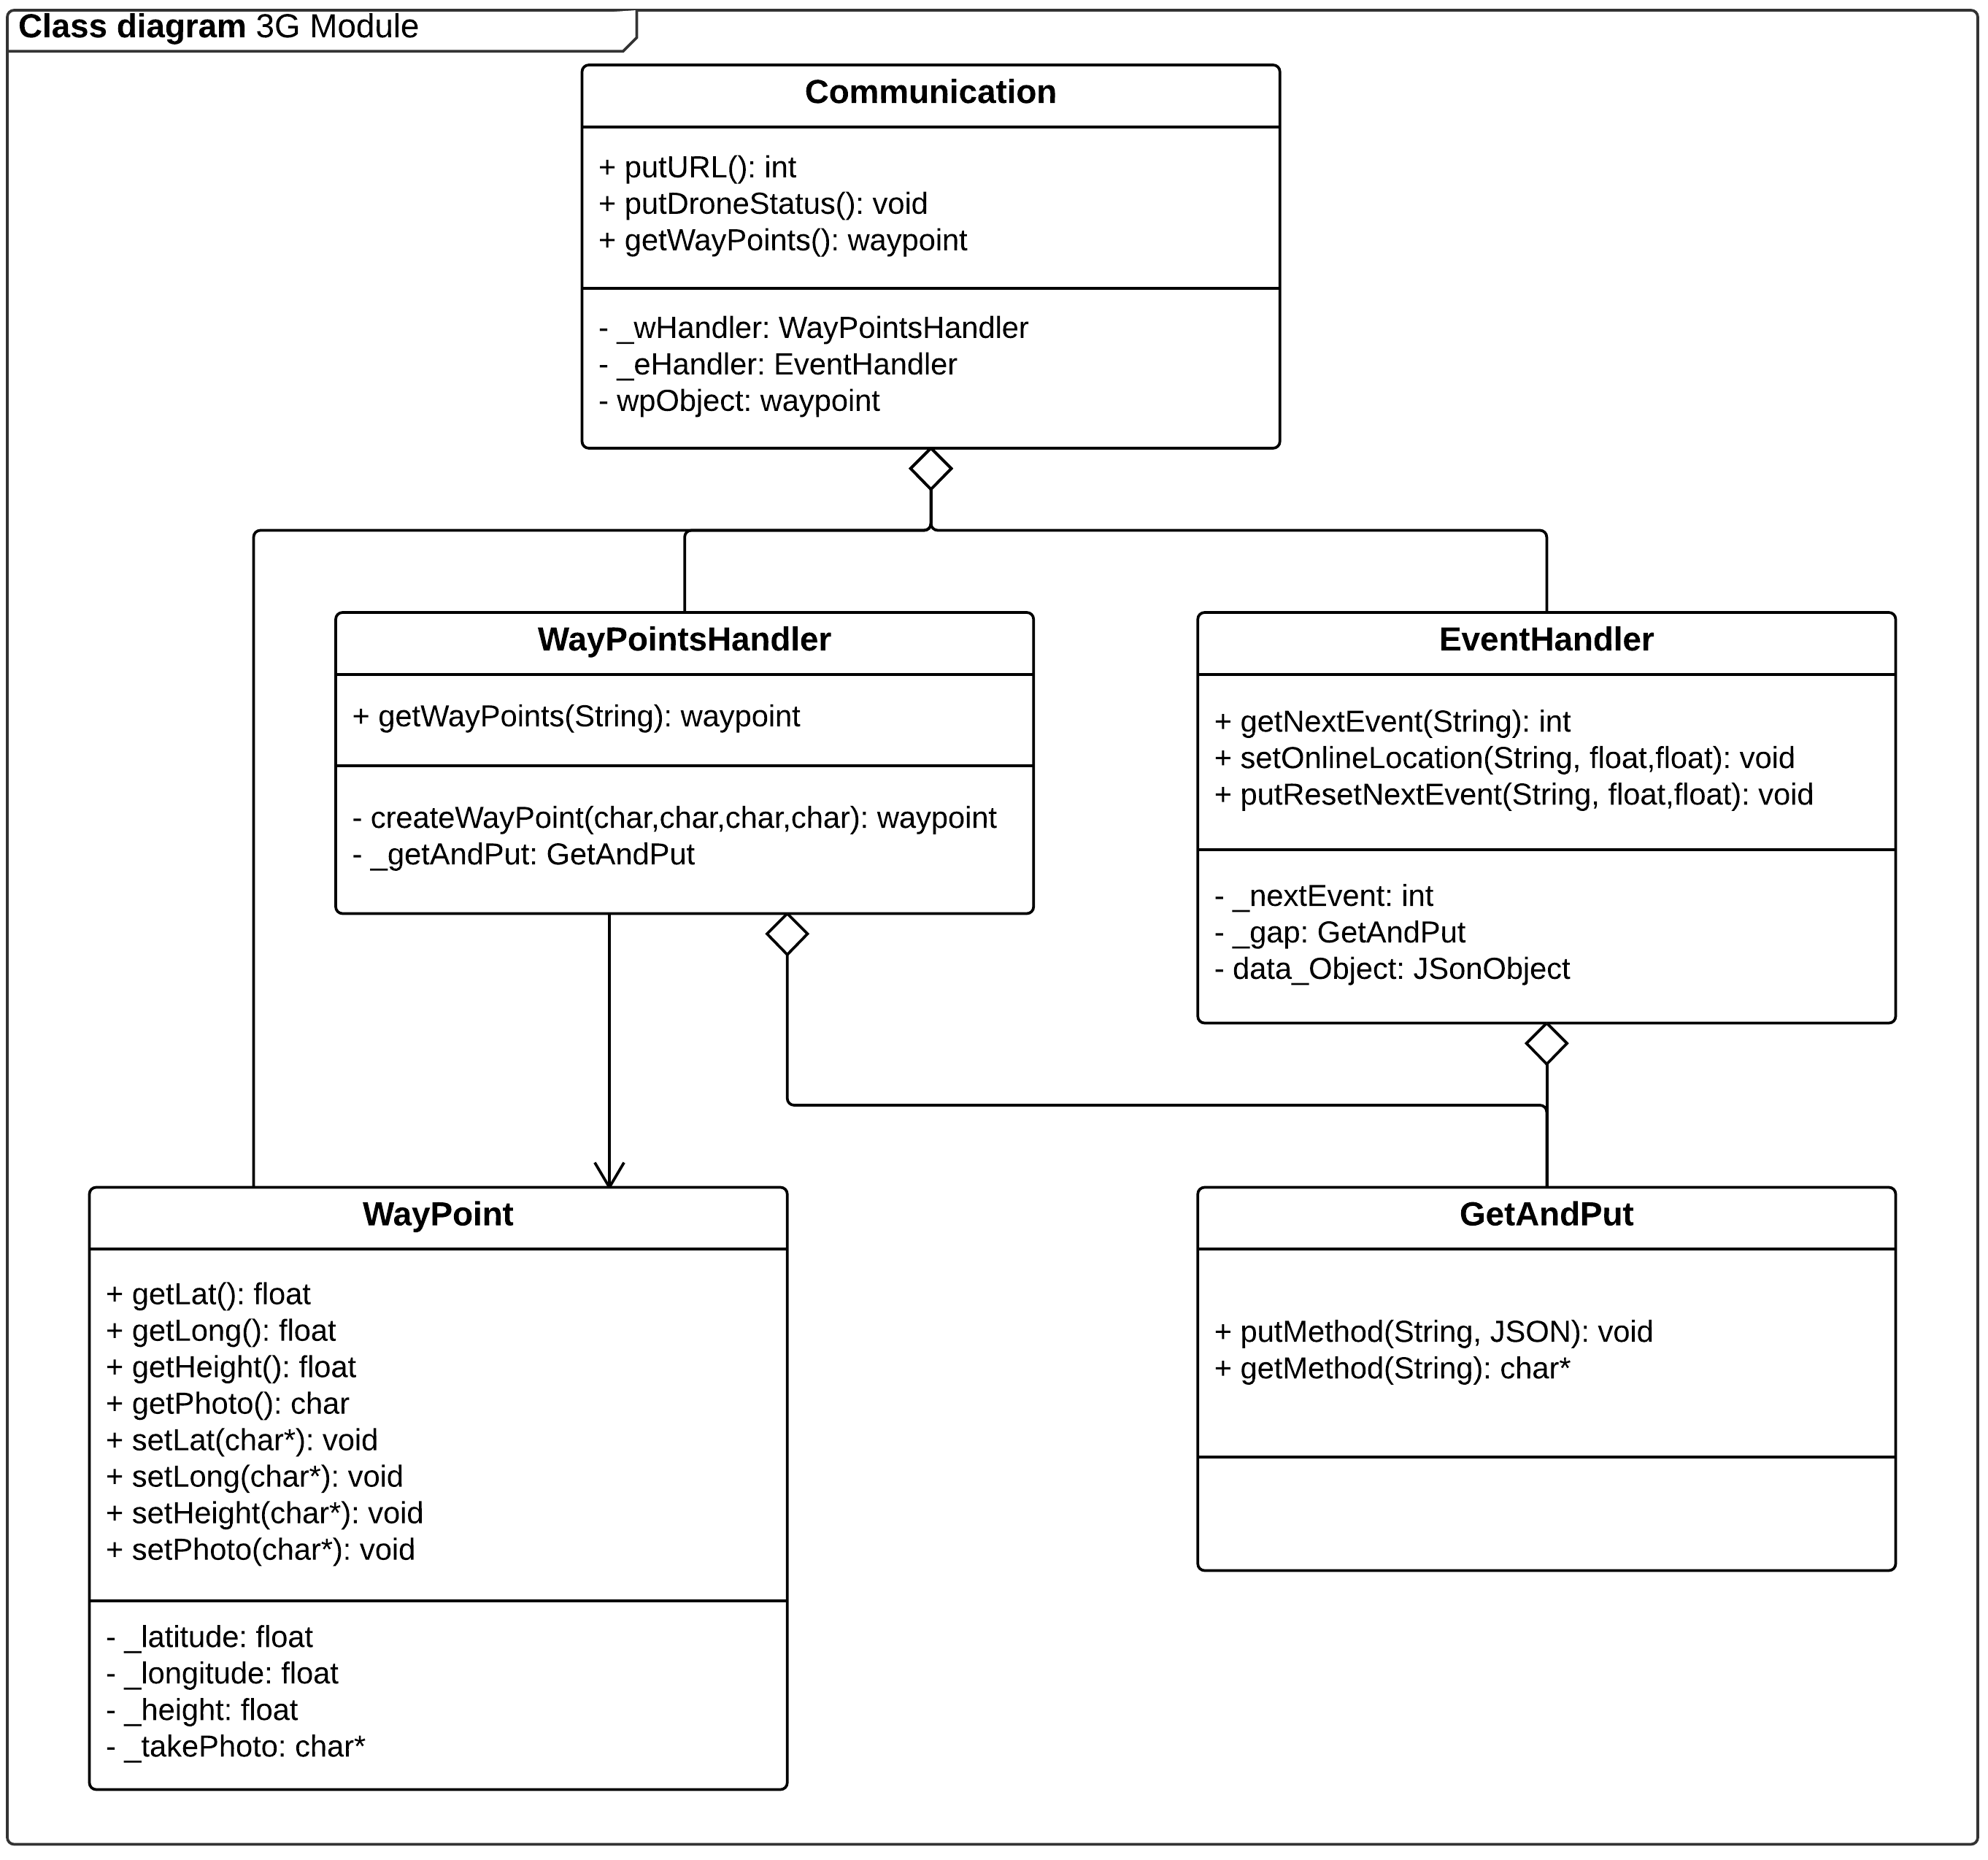
\includegraphics[width=1\textwidth]{Billeder/klasse_diagrammer/classdiagram_3gmodule.png}
	\vspace{0cm}
	\caption{Klassediagram 3G modul}
	\label{fig:classDiagram_3Gmodul}
\end{figure}


\textbf{GetAndPut} \\
GetAndPut klassen er den klasse der er tættest på hardwaren. Klassen indeholder de http metoder der bruges til kommunikation mellem dronen og serveren. 

\textbf{Communication} \\
Communication klassen er den øverste klasse og den håndterer sammen med andre klasser, alt der har med 3G at gøre.

\textbf{EventHandler} \\
EventHandleren er den klasse der håndterer Events. EventHandleren er bindeledet mellem communication- og GetAndPut klassen. EventHandleren sorterer eventID'et fra de data den modtager og returnerer værdien til communication klassen.

\newpage

\textbf{WayPointsHandler} \\
WayPointsHandler klassen er den klasse der håndterer de waypoints der hentes ned fra serveren. Klassen tager de waypoints den får fra serveren og gør dem tilgængeligt for resten af systemet. WayPointsHandleren bruger set metoderne i WayPoint klassen.

\textbf{WayPoint} \\
WayPoint klassen bruges til at kunne hente de forskellige waypoints ud af arrayet.  


\subsubsection*{Klassediagram webapplikation}
\vspace{-0.1cm}
På figur \ref{fig:classDiagram_home} ses klasse diagrammet tilhørende iteration to for websitet. Funktionaliteten er blevet udvidet med overblik over droner i systemet og deres status. Mulighed for at oprette events til den ønskede drone. 
\begin{figure}[H]
	\centering
	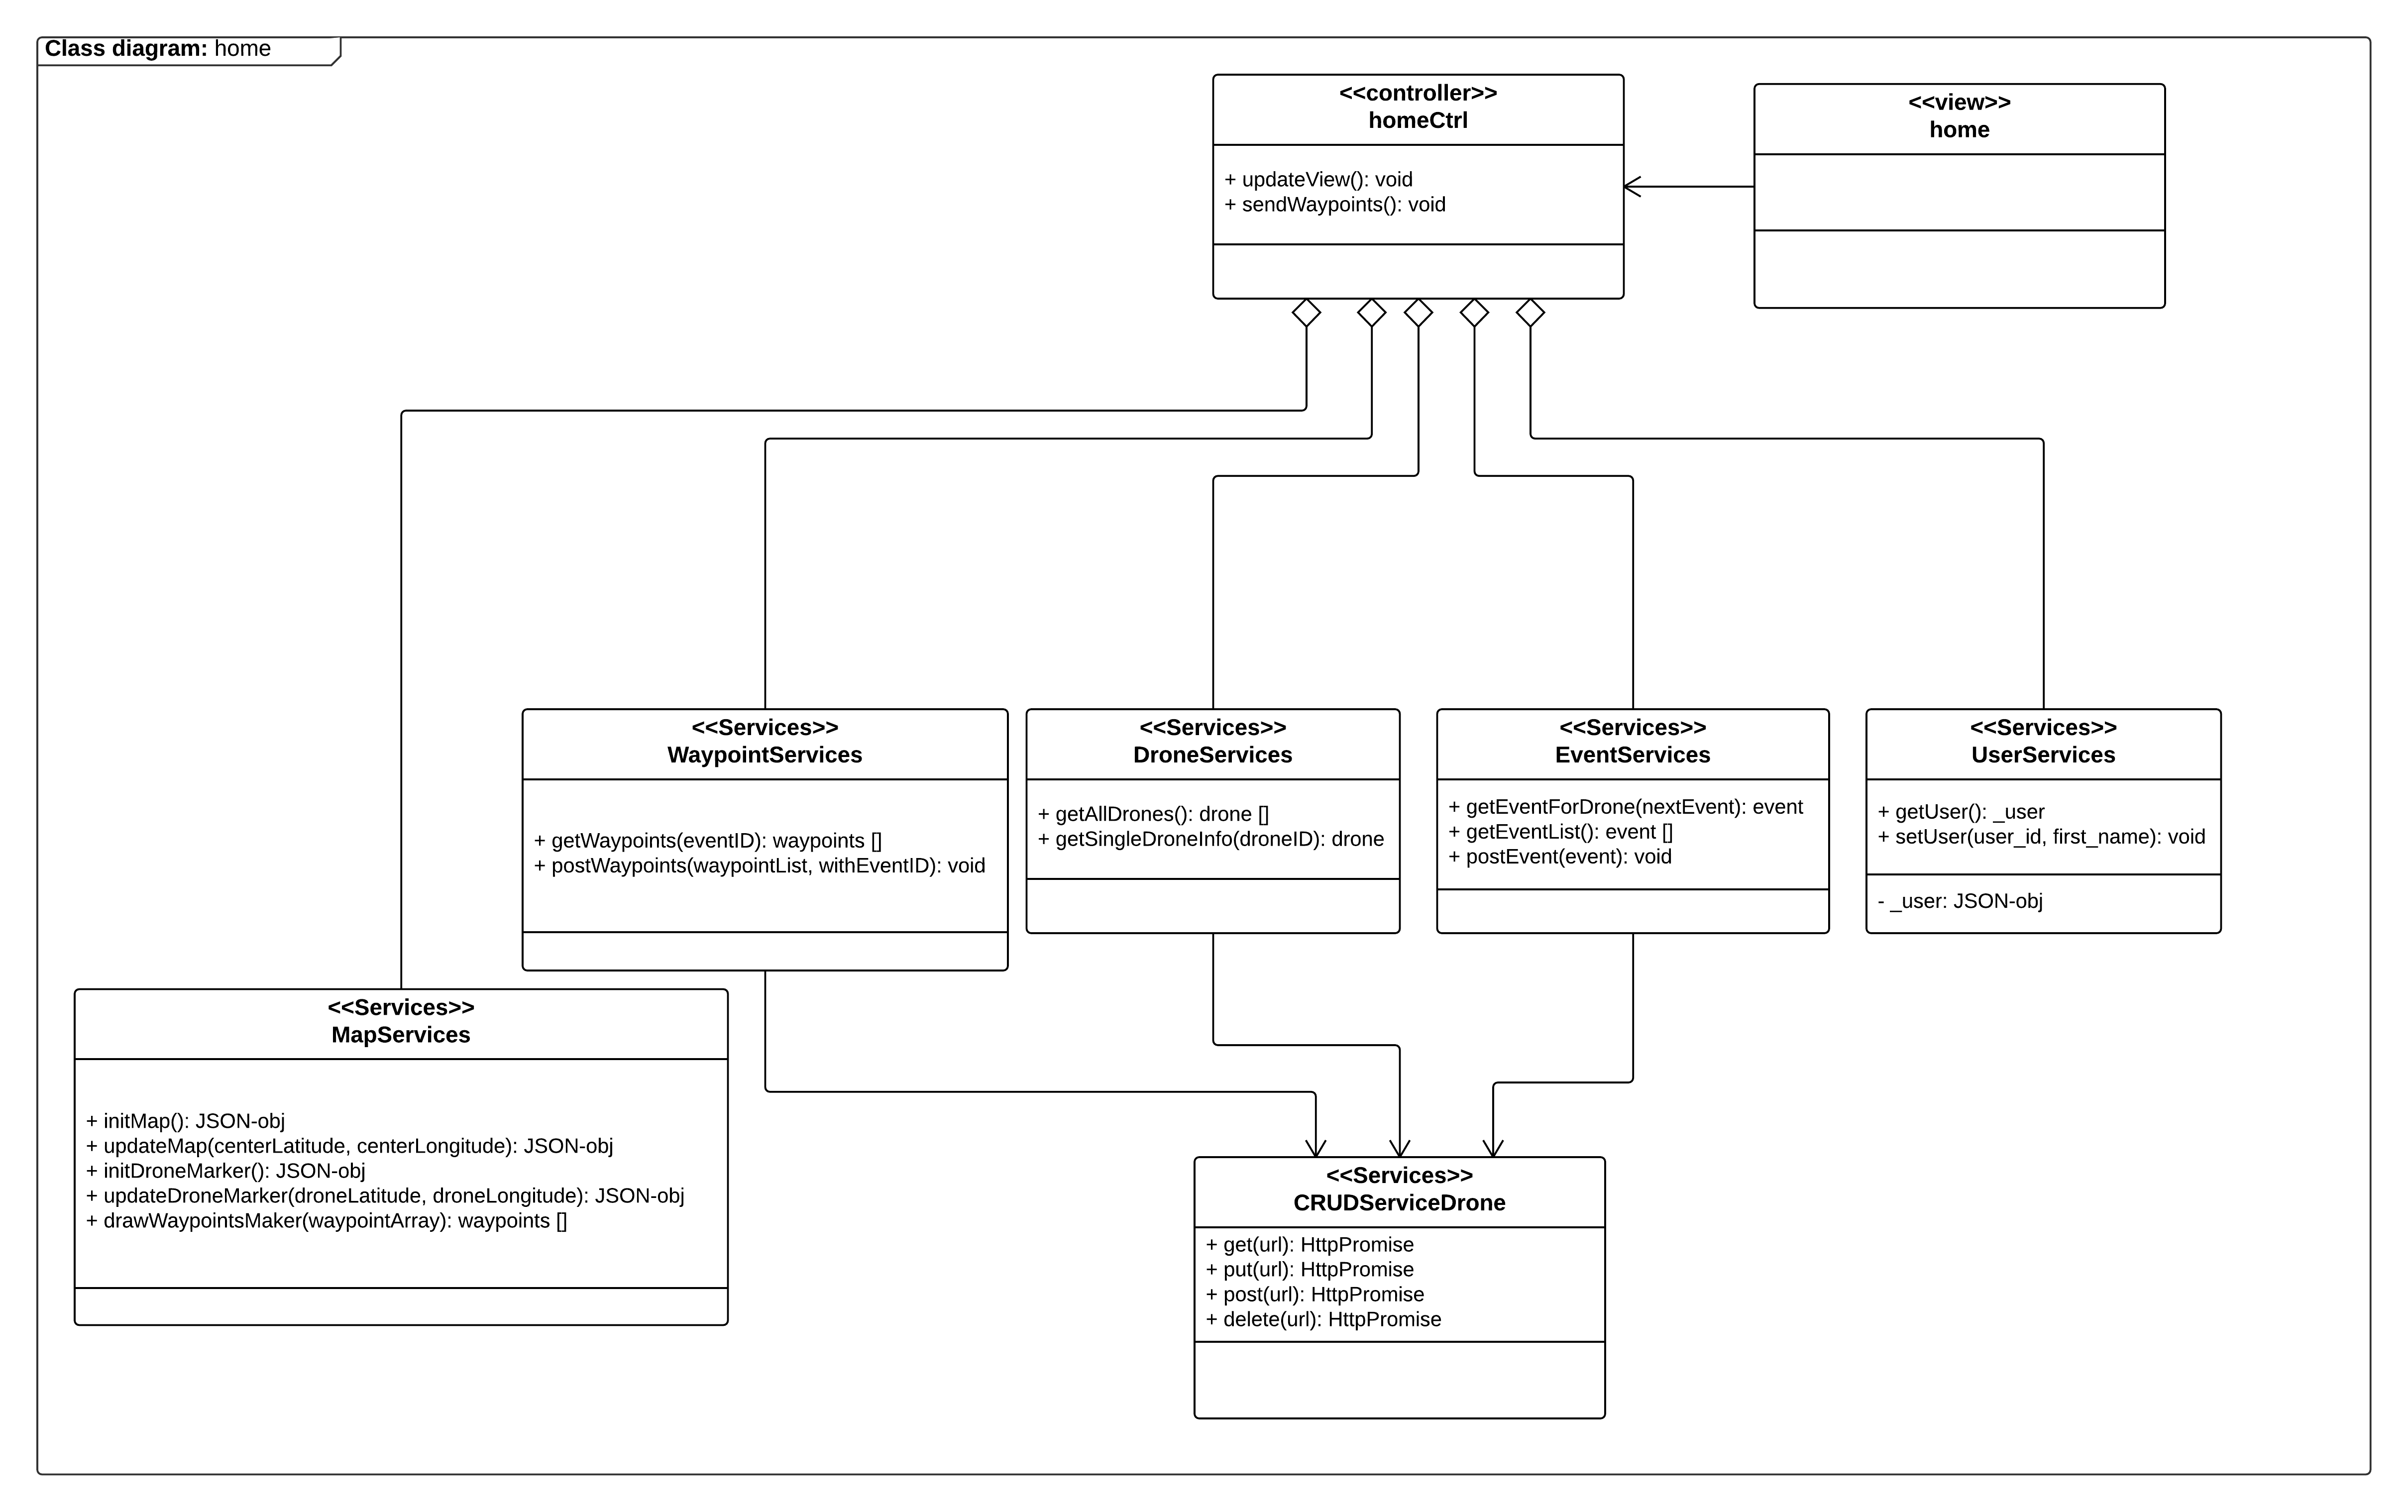
\includegraphics[width=1.\textwidth]{Billeder/klasse_diagrammer/home_class_diagram.png}
	\vspace{-0.5cm}
	\caption{Klassediagram home}
	\label{fig:classDiagram_home}
\end{figure}

\textbf{home}
Denne klasse er view'et tilhørende iteration to. Denne klasse sammen med homeCtrl skaber det endelig view som brugeren ser i sin browser når han besøger siden.

\textbf{homeCtrl}
HomeCtrl klassen er controller klassen til iteration to. Det er den eneste klasse der har direkte forbindelse til view'et, homeCtrl klassen deler også hukommelse med view'et igennem two-way-binding med scopes.

\textbf{DroneServices}
Denne klasse indeholder logikken om drone håndteringen. Den har ansvaret for at hente informationer omkring droner fra serveren via CRUDServiceDrone klassen.

\textbf{WaypointServices}
Denne klasse indeholder logikken om waypoint håndtering. Denne klasse henter henter waypoints tilhørende et event til controller klassen. Klassen bliver også brugt til at sende waypoints til serveren via CRUDServiceDrone klassen.

\textbf{EventServices}
Denne klasse indeholder logikken om event håndtering. Klassen bruges til at hente en event liste, et enkelt event for en givet drone og sende et nyoprettet event til serveren via CRUDServiceDrone klassen.

\textbf{MapServices}
Denne klasse indeholder logikken om map håndtering. Klassen bruges til at opdatere kortet i view'et, tegne waypoints og dronen på kortet.

\textbf{CRUDServicesDrone}
Denne klasse fungere som bindeled imellem server og webapplikation. Klassen indeholder alt logikken omkring kommunikation til serveren, alle der vil kommunikere med serveren i systemet skal benytte sig af denne klasse. Igennem denne service er det muligt at hente, opdater og poste data til serveren.

\textbf{UserServices}
Denne klasse blev oprettet i iteration et og bruges til at gemme information omkring hvilke bruger der er logget ind i systemet.

\newpage
\subsection{Iteration \#3}
I iteration 3 arbejdes med blokke som skal håndterer hvordan der tages billeder, forsendelse af billeder og billede visning. Der monteres kamera på dronen, så den under flyvning kan tage billeder ved de GPS lokationer som bruger har defineret i flyveopsætningen. Alle billeder der tages under flyvning sendes via mobilnet fra dronen til server. Websiden henter automatisk de seneste billeder fra serveren og gør disse tilgængelige for bruger. Hvordan systemet er tiltænkt at bruges beskrives i user story nedenfor:

\subsubsection*{User story}
Under flyvning tager dronen billeder som sendes via 3G/GPS modulet til serveren. Websiden kontrollerer løbende hvilke billeder der er findes på serveren og gør disse tilgængelig for bruger. Login er påkrævet før bruger kan få lov at se billeder fra forskellige flyvninger. Efter succesfuld login på websiden vælger bruger historik og vises information fra tidligere flyvninger. 

%kommentar
\begin{figure}[H]
	\centering
	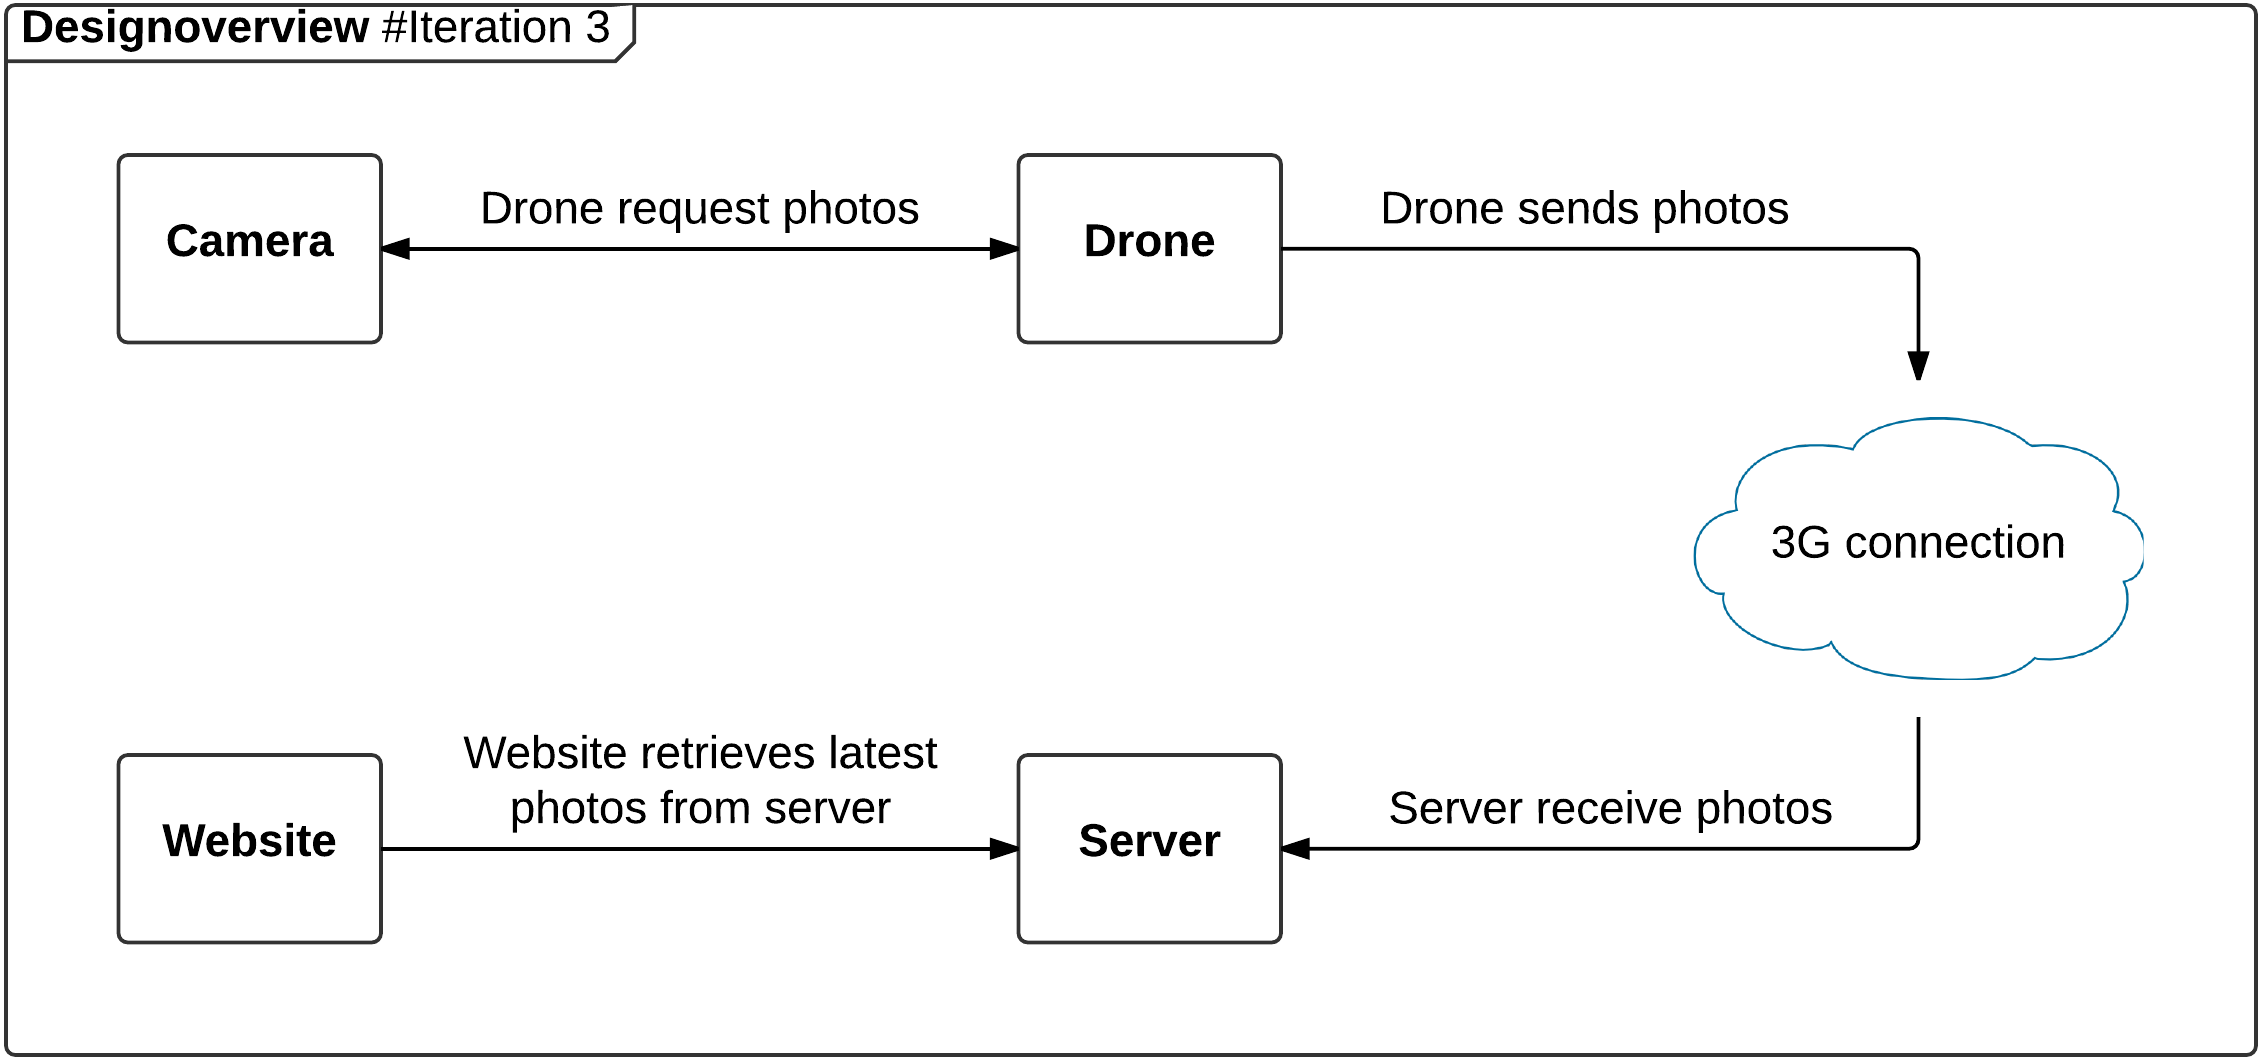
\includegraphics[width=1\textwidth]{Billeder/design_overview/design_overview_iteration3.png}
	\vspace{-.5cm}
	\caption{Designoverview \#iteration 3}
	\label{fig:design_overview_UC1}
\end{figure}
\newpage

\newpage
\subsubsection*{Pakkediagram drone}
I dette afsnit vises pakkediagram tilhørende drone. Hver pakke i pakkediagrammet består af en eller flere klasser, der med stort samspil udfører opgaver indenfor et fælles ansvarsområde. 
På hver pakke findes en lille beskrivelse, der tydeliggør pakkens ansvarsområde. De dele af pakkerne der er gråskraveret, er funktionalitet udarbejdet i tidligere iteration.


\begin{figure}[H]
	\centering
	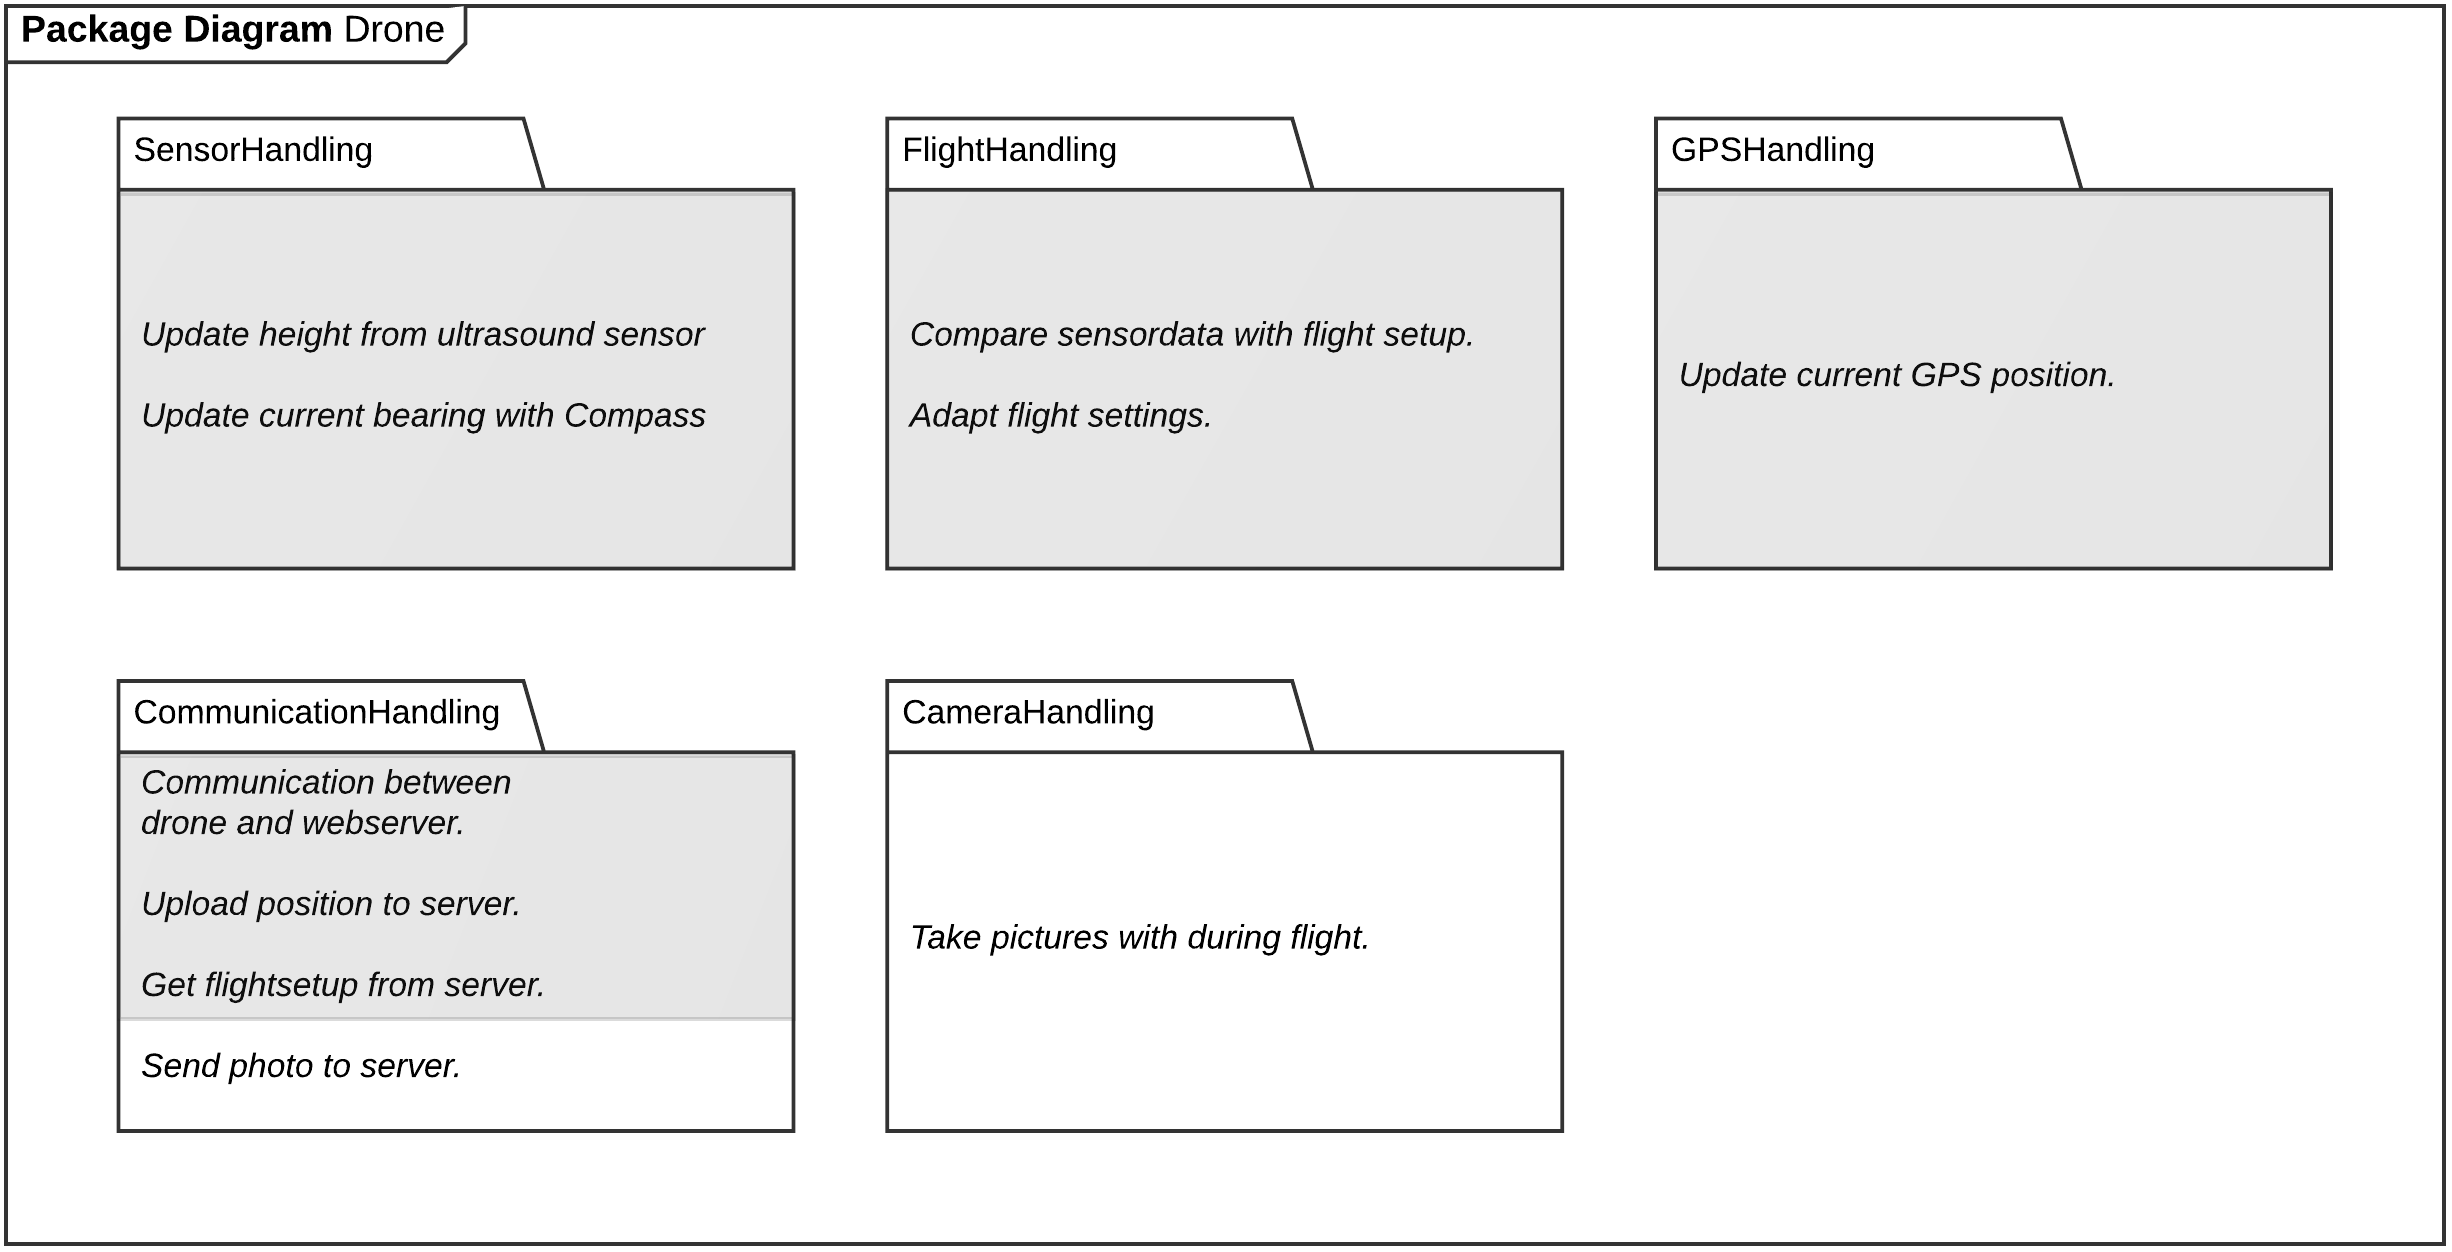
\includegraphics[width=1\textwidth]{Billeder/pakke_diagrammer/iteration3_drone.png}
	\vspace{-0.5cm}
	\caption{Pakkediagram drone}
	\label{fig:iteration2_pakke_diagram_drone}
\end{figure}

\textbf{SensorHandling}\\
Pakken er ansvarlig for indsamling af sensor data. I denne iteration skal pakken bruges til aflæsning af højdemåler og kompasset på flight control boardet. 

\textbf{FlightHandling}\\
Pakkens ansvar er kontrol og styring af drone under flyvning. Ved sammenligning af sensor data og data fra flyveopsætning tilpasses flyvehøjde, orientering mm

\textbf{GPSHandling}\\
Pakkens ansvar er håndtering af GPS. Dels er pakken ansvarlig for opstart og initiering af GPS, og desuden bruges pakken hver gang dronens nuværende GPS position skal opdateres.

\textbf{CommunicationHandling}\\
Pakkens ansvar er kommunikation imellem drone og server. Efter denne iteration skal dronen kunne hente flyveopsætninger fra server, sende sin nuværende GPS position til server og sende billeder til server.

\textbf{CameraHandling}\\
Pakkens ansvar er håndtering af kamera. Pakken bruges til at starte, initierer, bruge og slukke kameraet.


\newpage
\subsubsection*{Pakkediagram webapplikation}
I dette afsnit vises pakkediagram tilhørende webapplikation. Hver pakke i pakkediagrammet består af en eller flere klasser, der med stort samspil udfører opgaver indenfor et fælles ansvarsområde. 
På hver pakke findes en lille beskrivelse, der tydeliggør pakkens ansvarsområde. De dele af pakkerne der er gråskraveret, er funktionalitet udarbejdet i tidligere iteration. 

\begin{figure}[H]
	\centering
	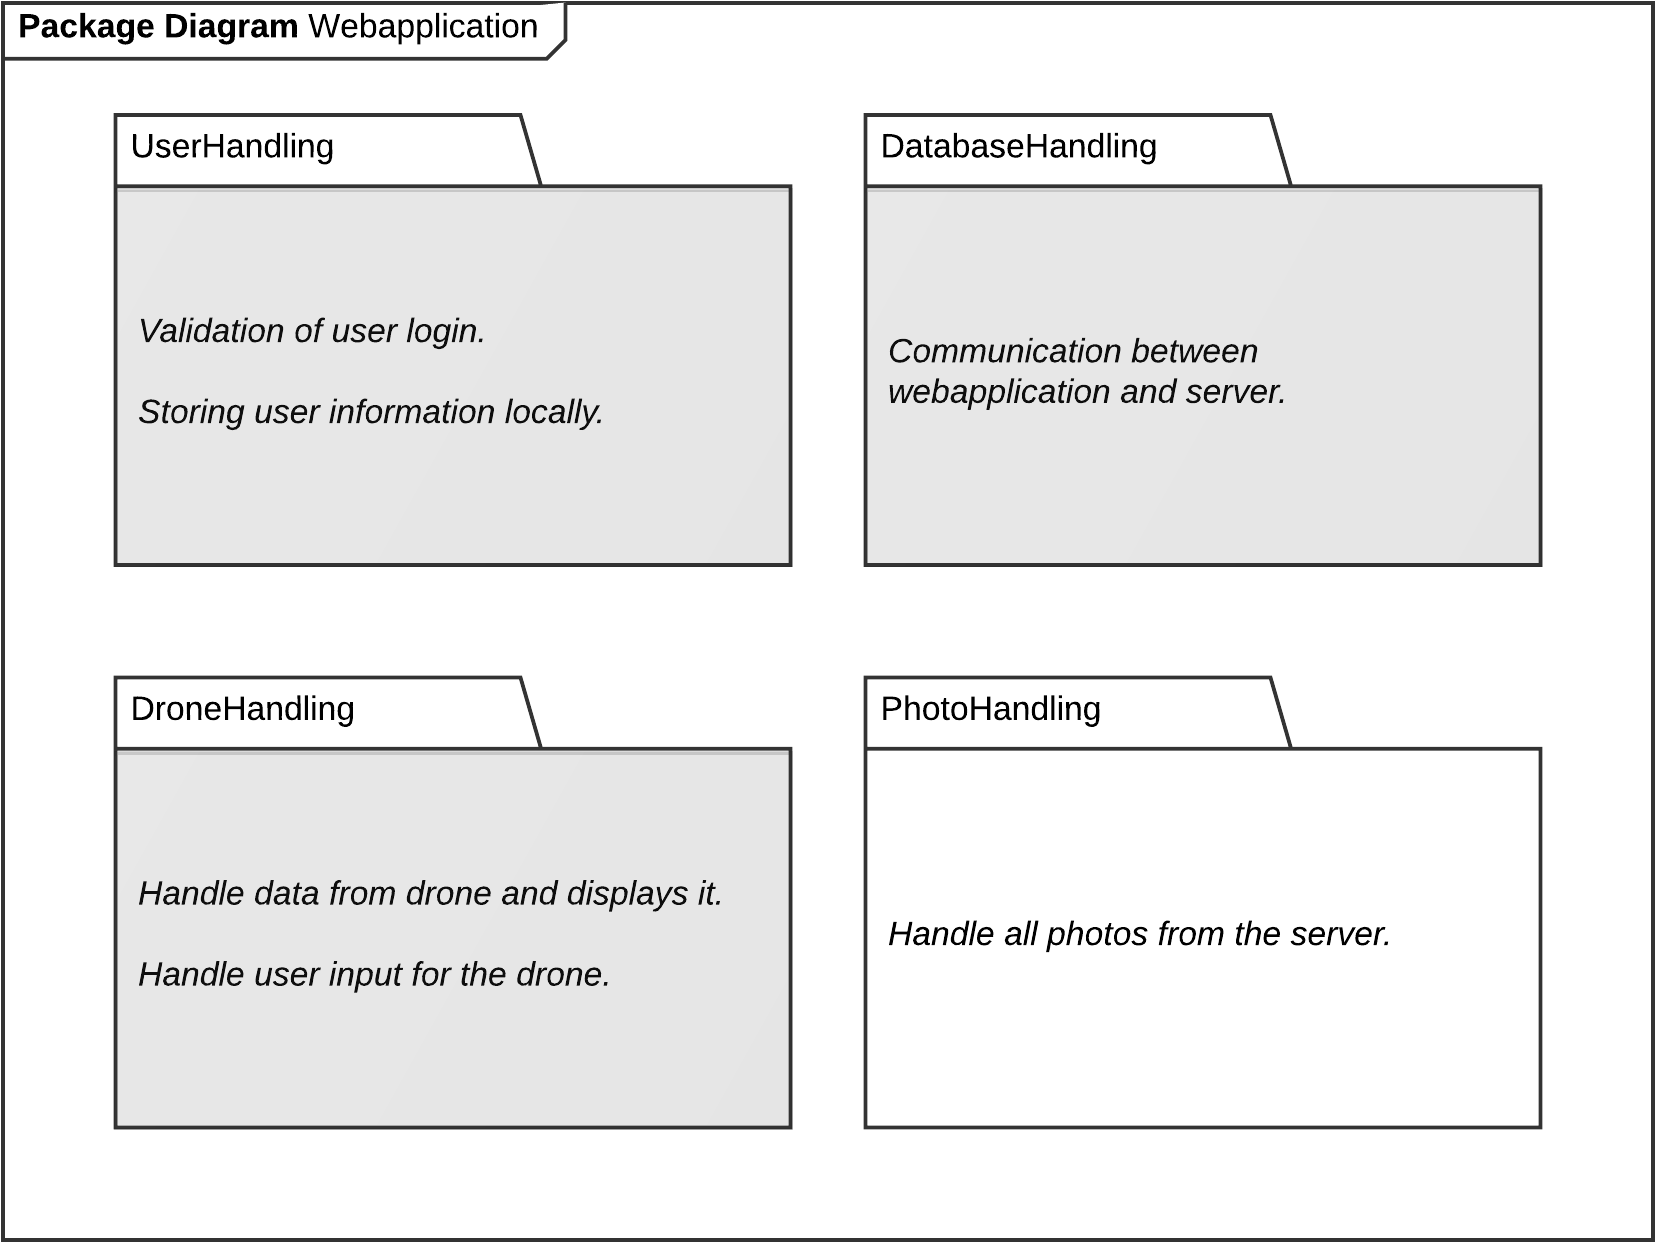
\includegraphics[width=1\textwidth]{Billeder/pakke_diagrammer/iteration3_server.png}
	\vspace{-0.5cm}
	\caption{Pakkediagram webapplikation}
	\label{fig:iteration3_pakke_diagram_webapplikation}
\end{figure}

\textbf{UserHandling}\\
Pakkens ansvar er validering af login/log ud på websitet. Pakken har også ansvaret for at hente og gemme data om den pågældende bruger.

\textbf{DatabaseHandling}\\
Pakkens ansvar er kommunikation imellem databasen og serveren. 

\textbf{DroneHandling}\\
Pakkens ansvar er alt data vedrørende dronen, så som håndteringen af events, waypoints og div droner.

\textbf{PhotoHandling}\\
Pakkens ansvar er at håndtere de billeder dronen har taget under flyvning og præsentere dem for brugeren.

\newpage

\subsubsection*{Sekvens diagram}
\vspace{-0.3cm}
På sekvensdiagrammet på figur \ref{fig:Sekvens_diagram_iteration3}, vises hvilke klasser der indgår og bruges i tredje iteration. På sekvensdiagrammet vises det hvordan kamera delen af 3G/GPS modulet håndteres og hvordan ny tagede billeder sendes med post request til serveren. 

\vspace{-0.2cm}
%kommentar
\begin{figure}[H]
	\centering
	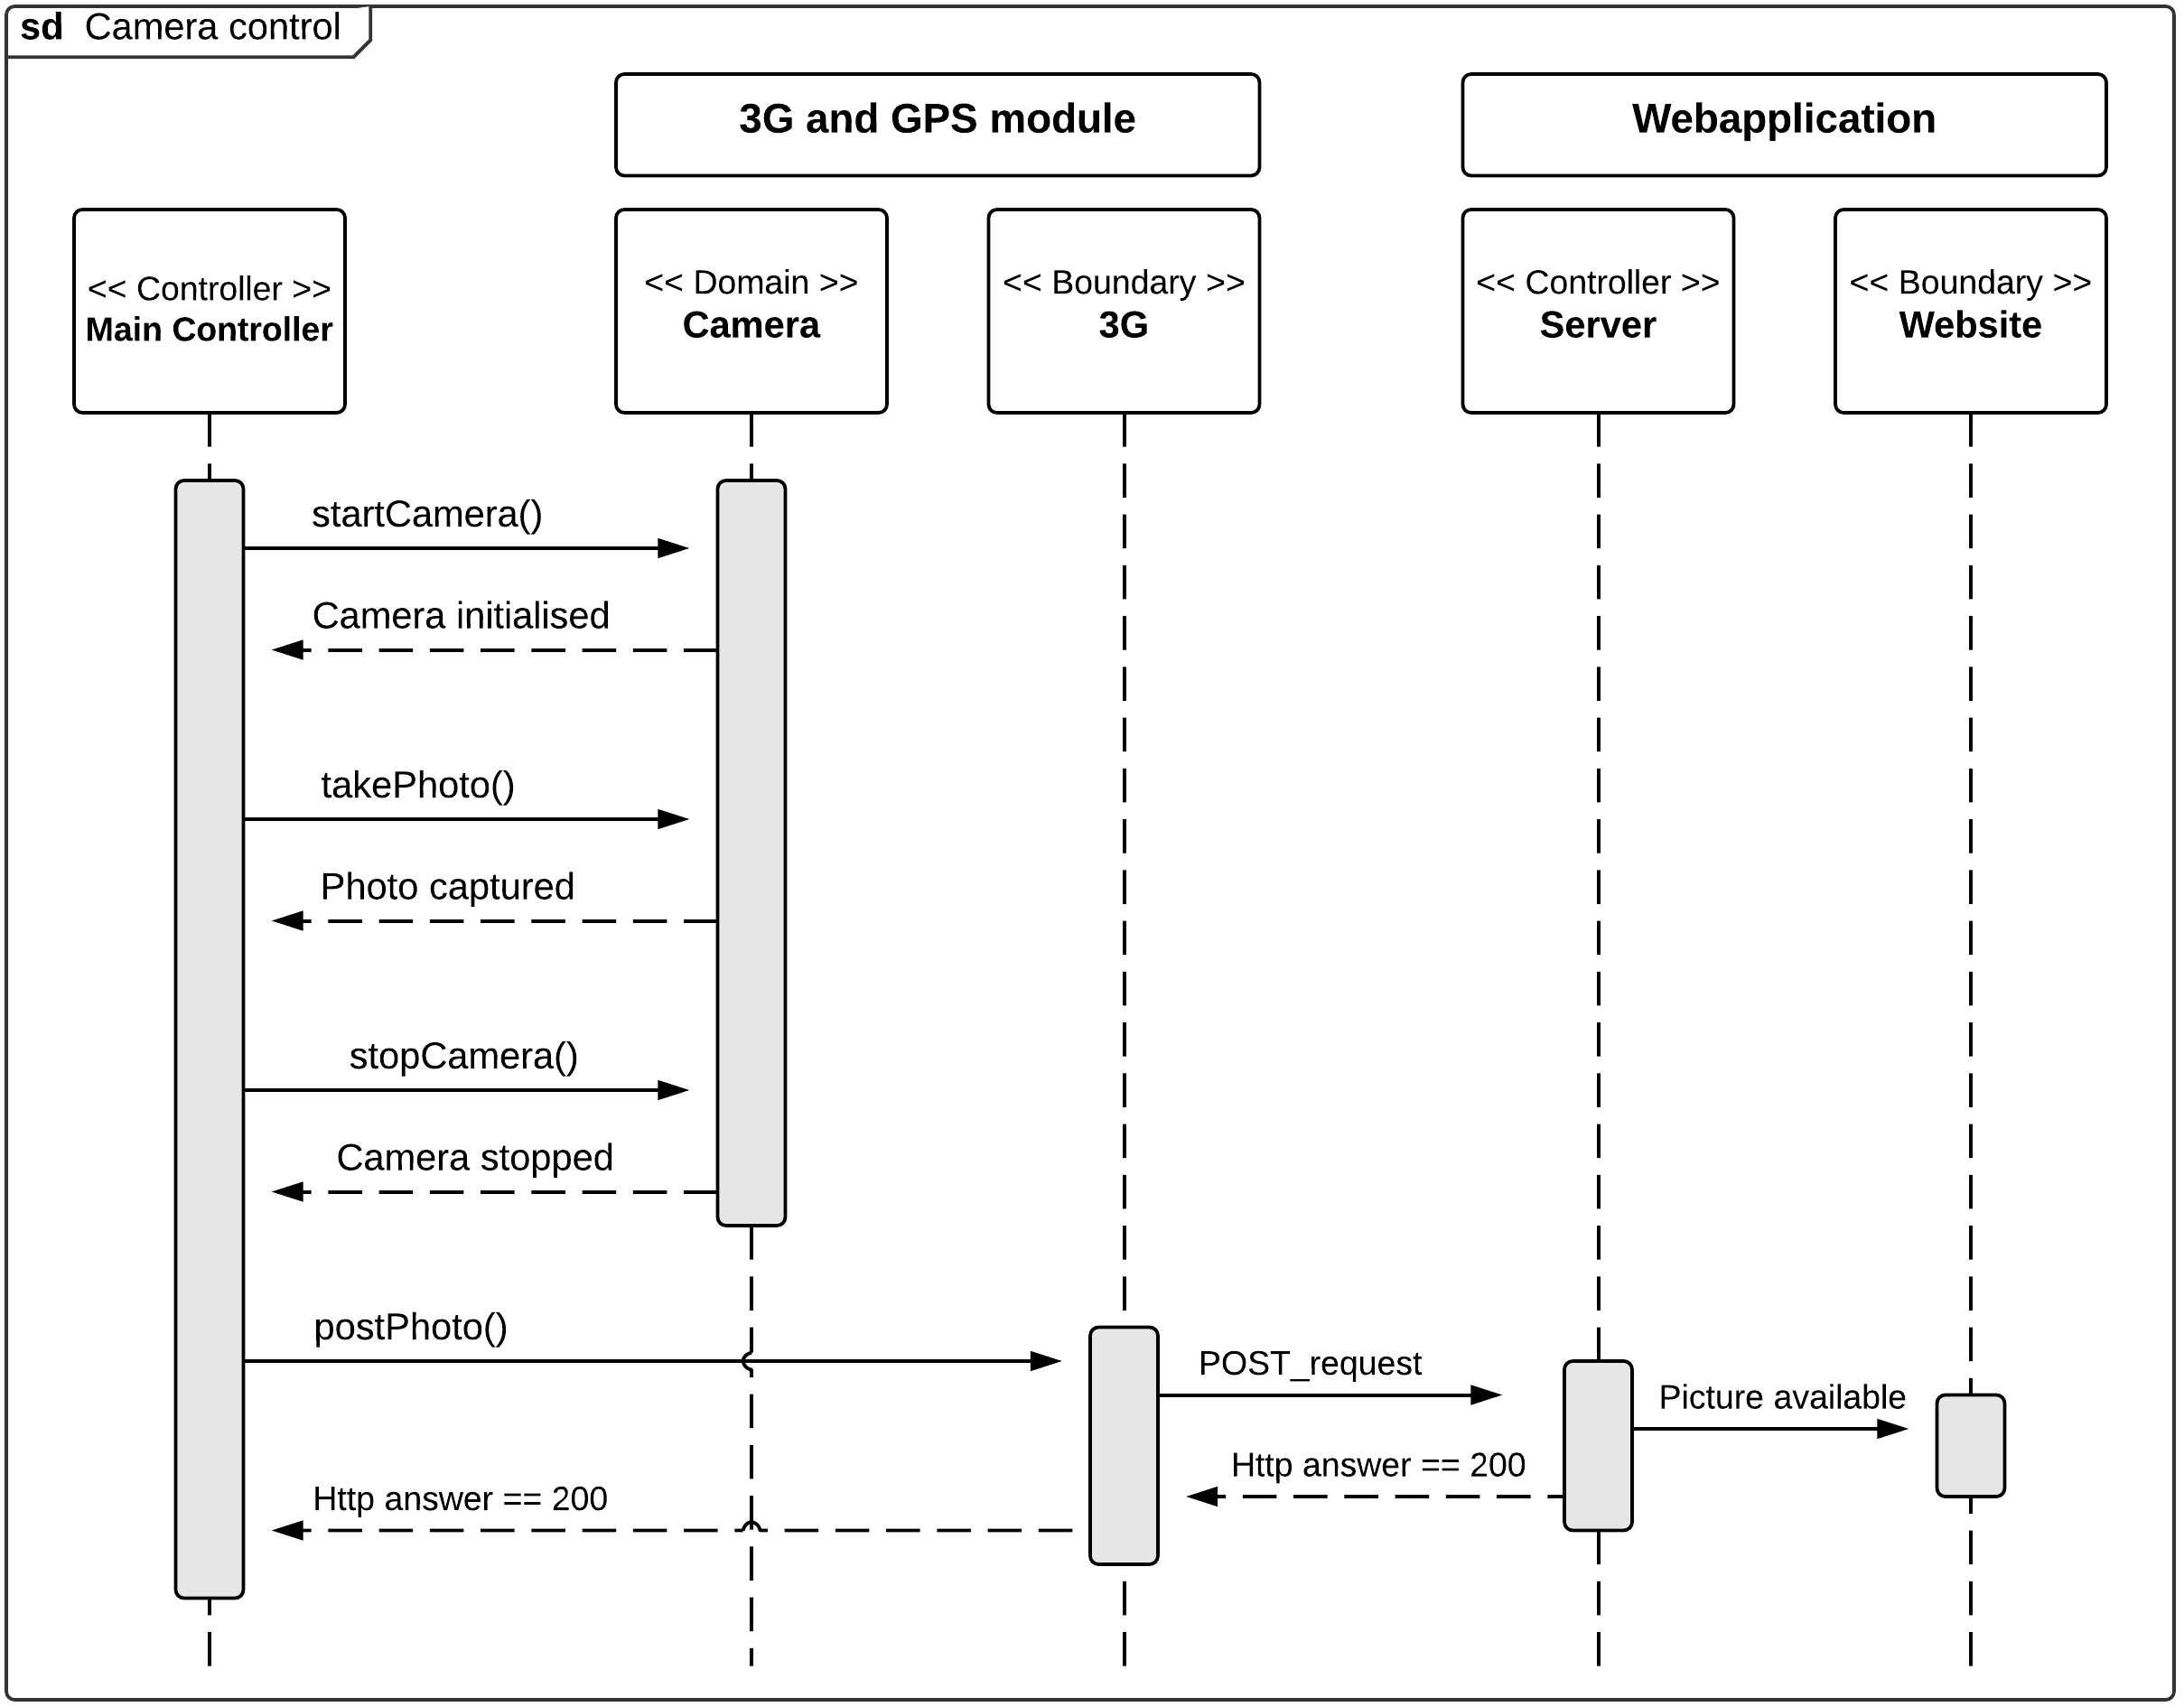
\includegraphics[width=1\textwidth]{Billeder/sekvens/sekvens_iteration3}
	\caption{Sekvens diagram \#iteration 3}
	\label{fig:Sekvens_diagram_iteration3}
\end{figure}
\vspace{-0.2cm}

\newpage

\subsubsection*{Klassediagram drone}

Figur \ref{fig:classDiagram_iteration3} vises et klassediagram tilhørende iteration 3. Klassediagrammet viser foruden main.cpp filen iteration 3's eneste centrale klasse og dens tilhørende metode. 

%kommentar
\begin{figure}[H]
	\centering
	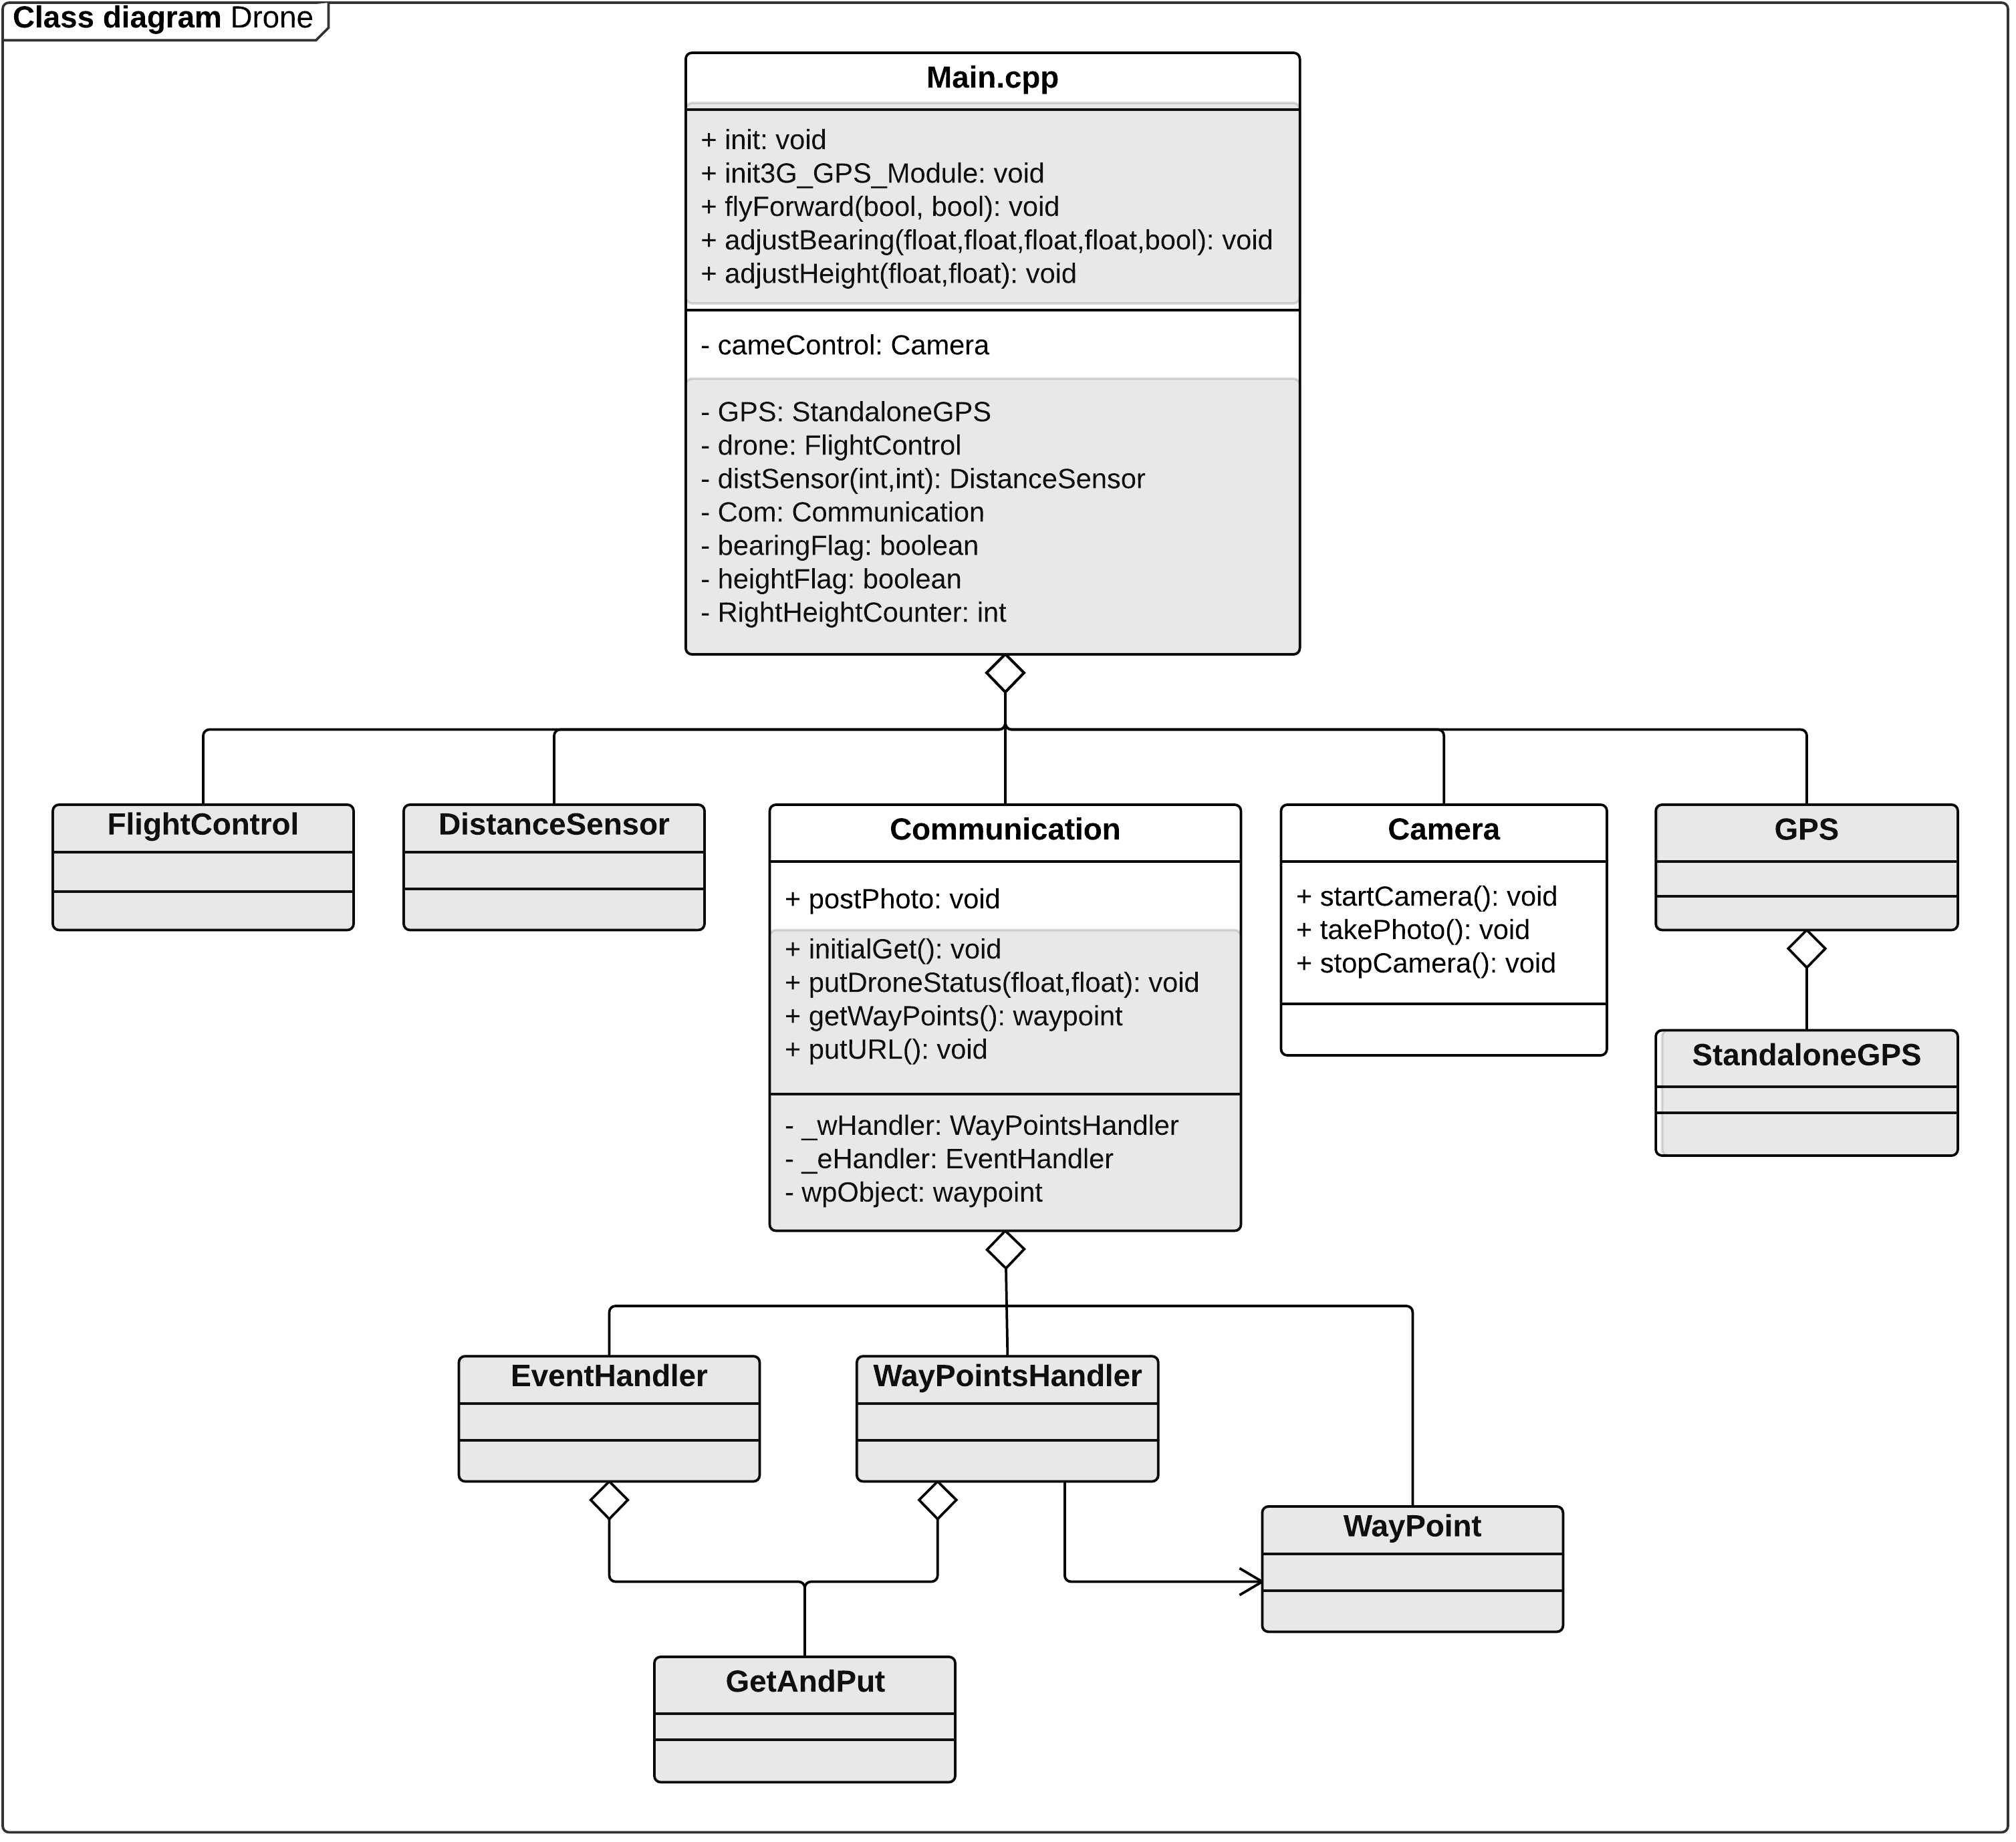
\includegraphics[width=1\textwidth]{Billeder/klasse_diagrammer/classdiagram_iteration3_drone.png}
	\vspace{-0.5cm}
	\caption{Klassediagram \#iteration 3}
	\label{fig:classDiagram_iteration3}
\end{figure}

\textbf{Main.cpp} \\
Main.cpp filen bruges til at oprette objekter af de Anti collision klassen og til at kalde dens tilhørende funktioner.

\textbf{Camera} \\
Klassen eneste funktion er at kontrollere afstanden til eventuelle objekter foran dronen. 


\newpage

\subsubsection*{Klassediagram webapplikation}

Figur \ref{fig:classDiagram_iteration3} vises klassediagrammet tilhørende iteration 3 for webapplikationen. 

%kommentar
\begin{figure}[H]
	\centering
	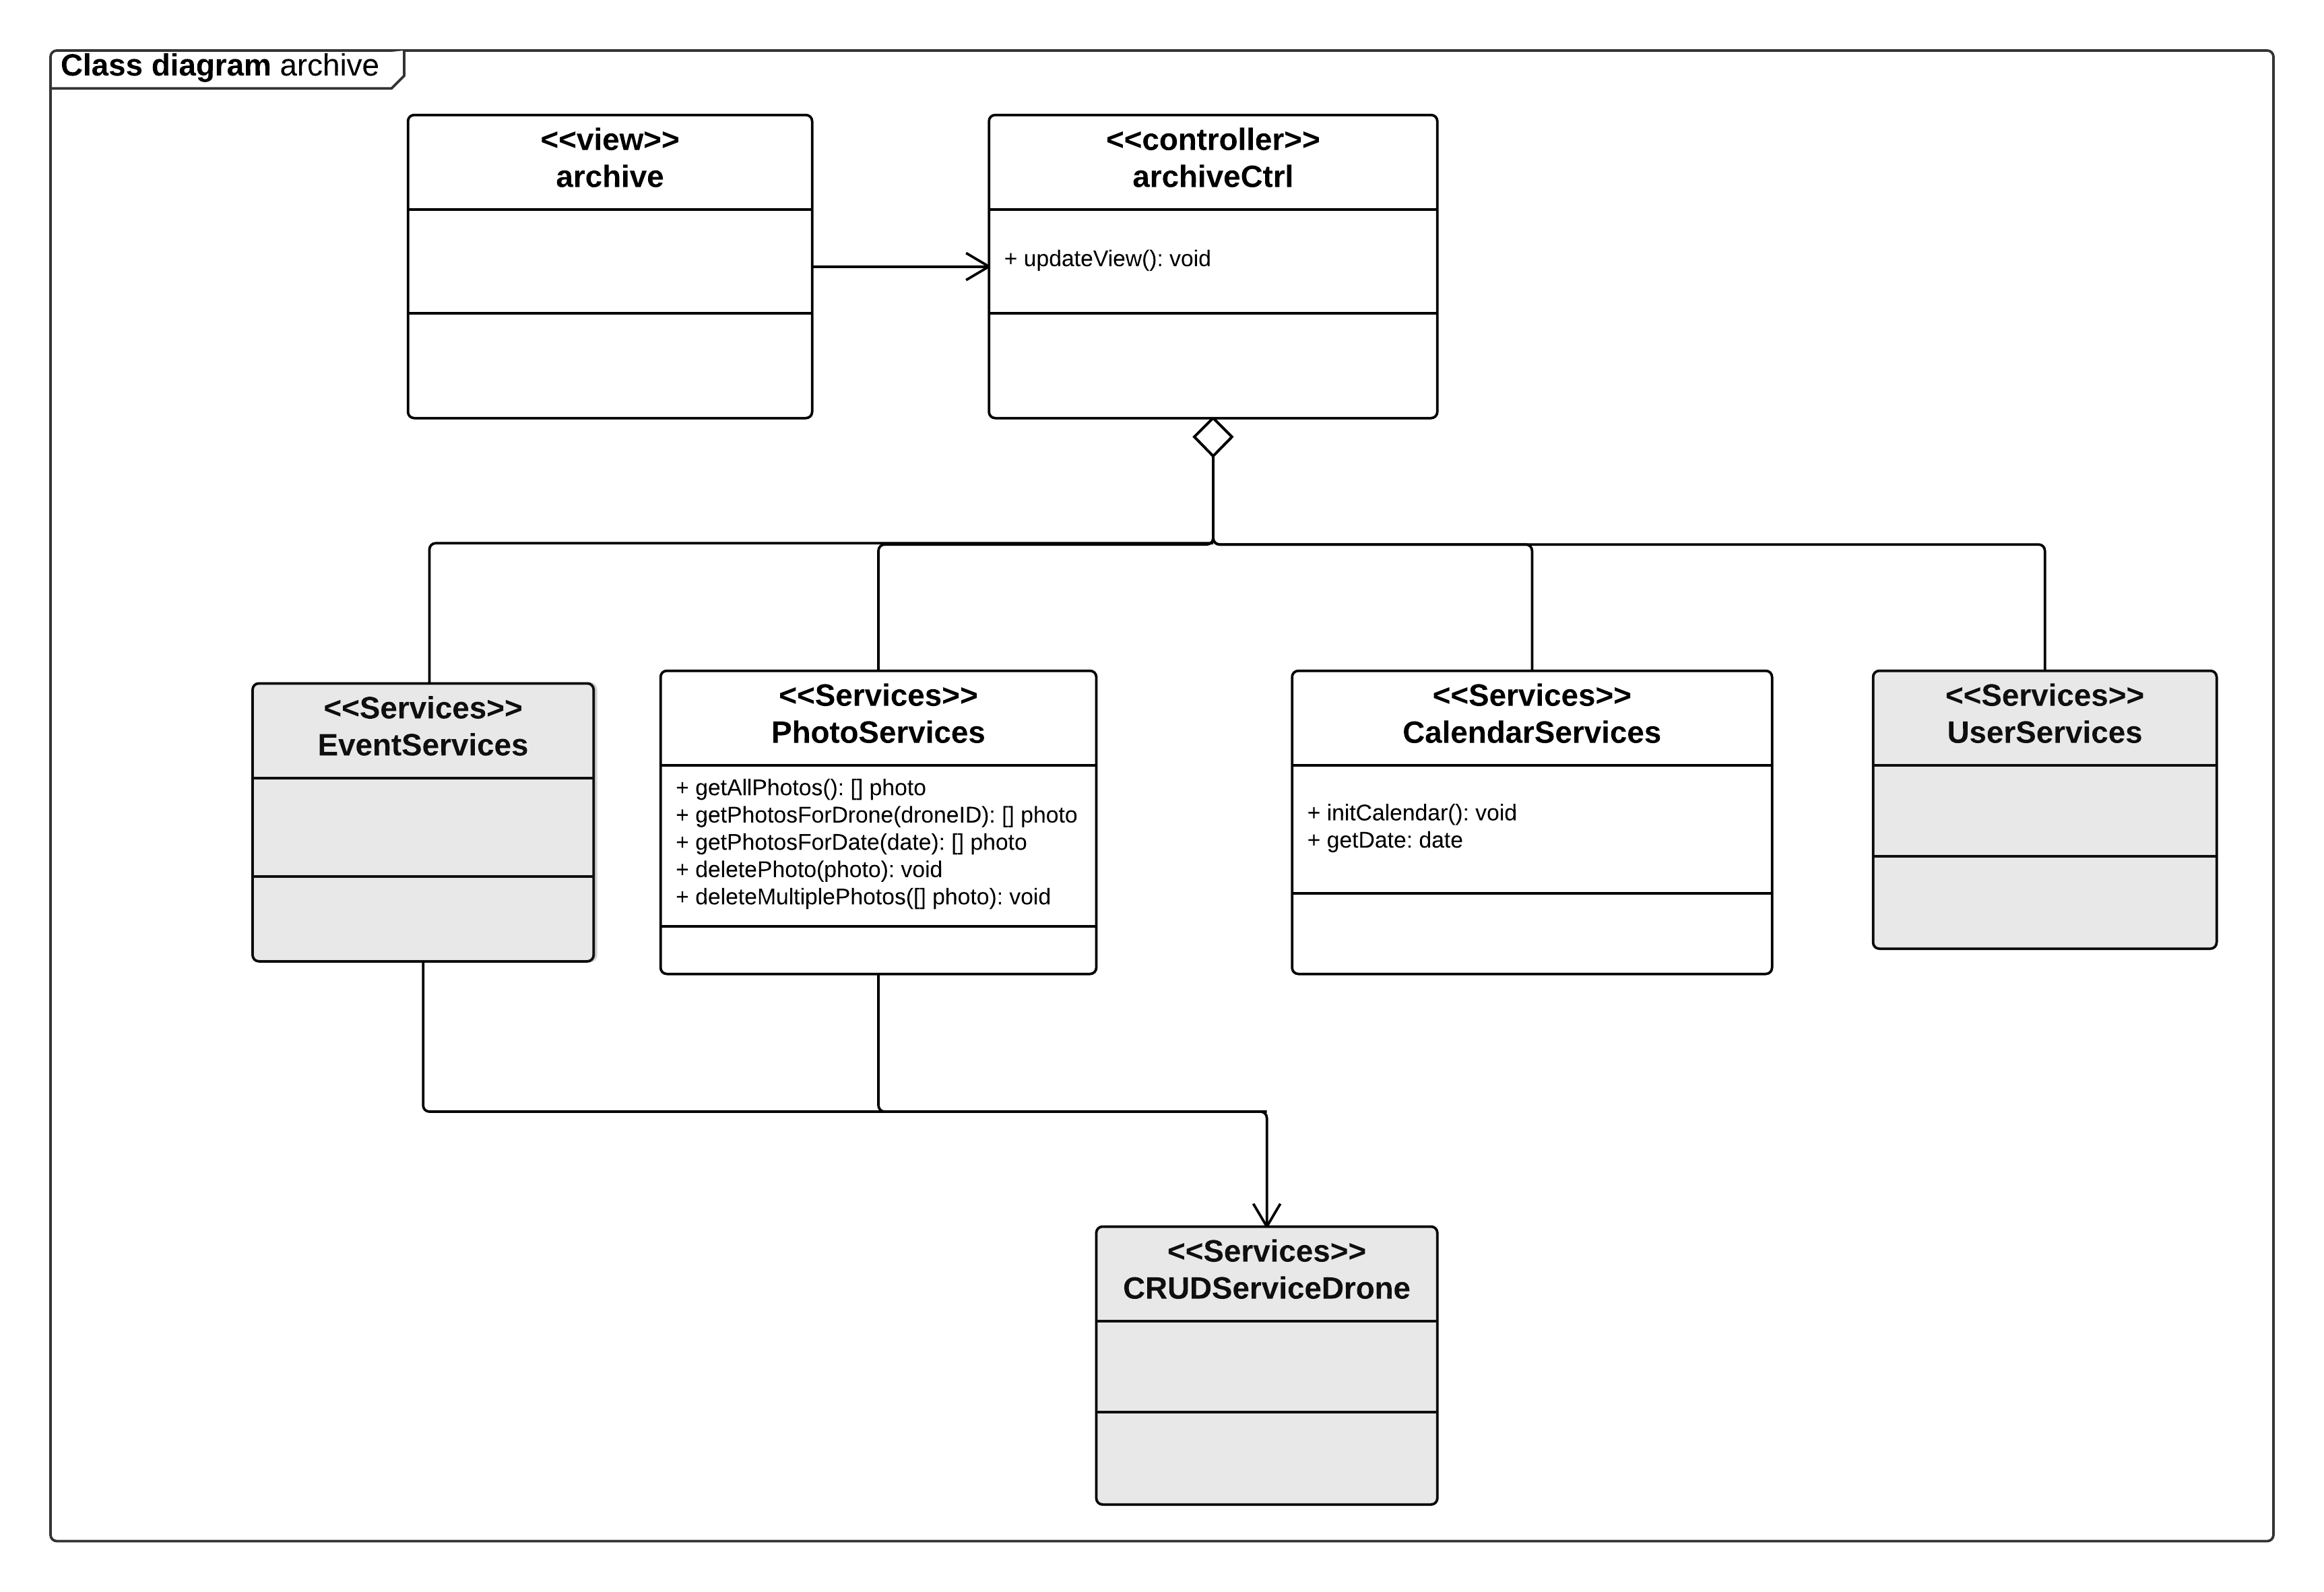
\includegraphics[width=1\textwidth]{Billeder/klasse_diagrammer/classdiagram_iteration3_server.png}
	\vspace{-0.5cm}
	\caption{Klassediagram \#iteration 3}
	\label{fig:classDiagram_iteration3}
\end{figure}

\textbf{archive}\\
Denne klasse er view'et tilhørende iteration tre. Denne klasse sammen med archiveCtrl skaber det endelig view som brugeren ser i sin browser når han besøger siden.

\textbf{archiveCtrl}\\
ArchiveCtrl klassen er controller klassen til iteration tre. Det er den eneste klasse der har direkte forbindelse til view'et, archiveCtrl klassen deler også hukommelse med view'et igennem two-way-binding med scopes.

\textbf{EventServices}\\
Denne klasse indeholder logikken om event håndtering. Klassen bruges til at hente en event liste, et enkelt event for en givet drone og sende et nyoprettet event til serveren via CRUDServiceDrone klassen.

\textbf{PhotoServices}\\
Denne klasse indeholder logikken om foto håndtering. Klassen bruges til at hente fotos via CRUDServiceDrone klassen, PhotoServices har også ansvaret for at slette uønskede billeder.

\textbf{CalendarServices}\\
Denne klasse indeholder logikken for kalenderen i view'et, klassen bruges til at oprette en kalender og navigering i kalenderen. Desuden bruges den også til at fortælle hvilke dato brugeren har valgt når han ønsker at finde billeder taget fra en givet dato.

\newpage

\textbf{UserServices}\\
Denne klasse blev oprettet i iteration et og bruges til at gemme information omkring hvilke bruger der er logget ind i systemet.

\textbf{CRUDServicesDrone}\\
Denne klasse fungere som bindeled imellem server og webapplikation. Klassen indeholder alt logikken omkring kommunikation til serveren, alle der vil kommunikere med serveren i systemet skal benytte sig af denne klasse. Igennem denne service er det muligt at hente, opdater og poste data til serveren.

\vspace{0.3cm}

\subsubsection*{State machine diagram}
\vspace{-0.3cm}
I state machine diagrammet på figur \ref{fig:Statemachine_iteration3}, vises de to states der eksisterer i iteration 3 og hvordan flowet imellem dem ser ud. Der eksisterer givet vis kun 2 states i iteration 3, men state machinen er medtaget fordi den fint illustrerer systemflowet.

\vspace{-0.2cm}
%kommentar
\begin{figure}[H]
	\centering
	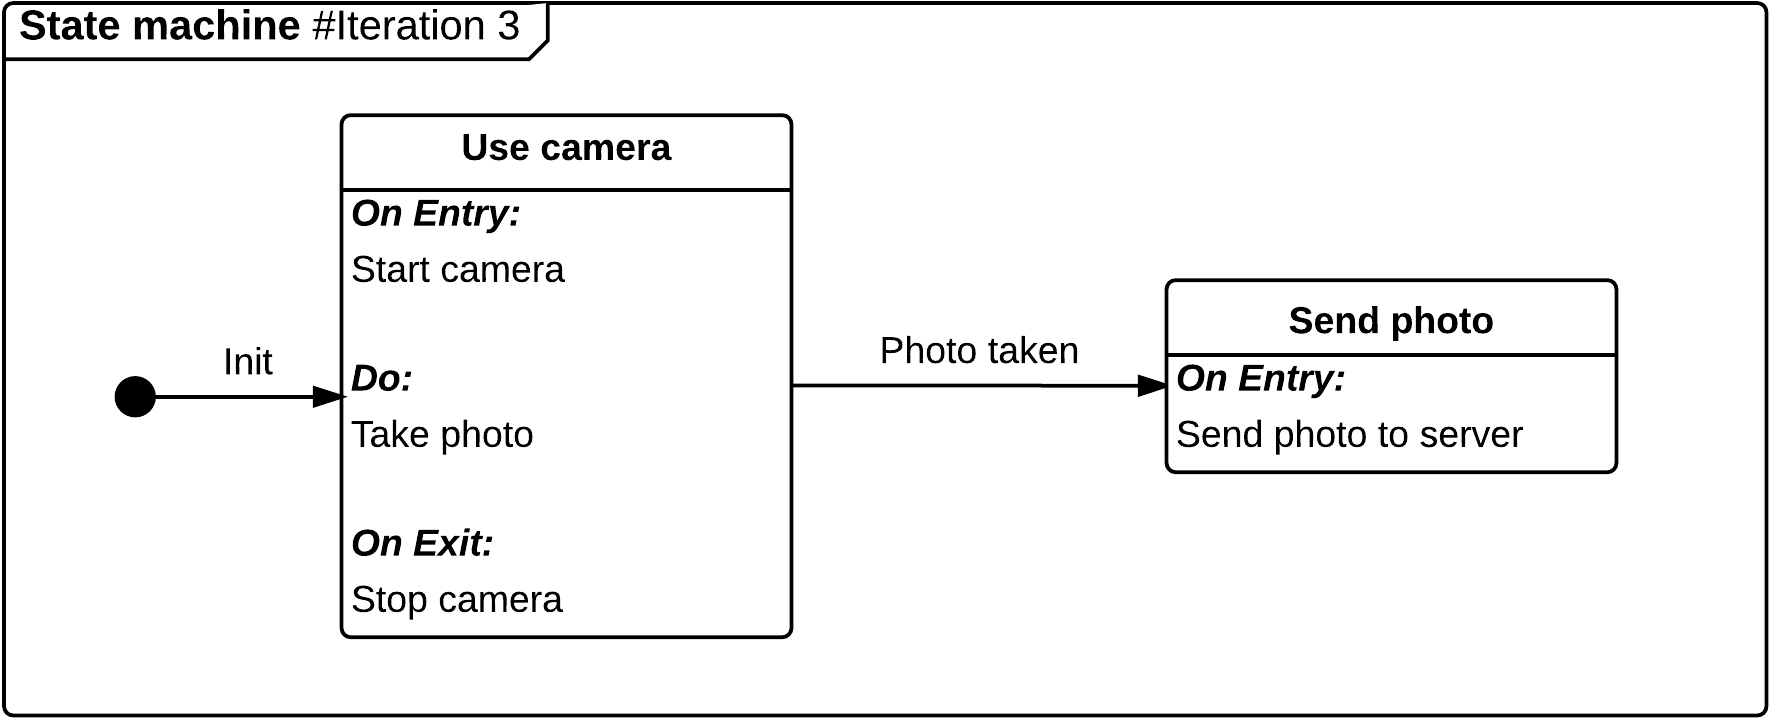
\includegraphics[width=0.9\textwidth]{Billeder/statemachine/State_iteration3.png}
	\caption{State machine \#iteration 3}
	\label{fig:Statemachine_iteration3}
\end{figure}



\newpage
\subsection{Iteration \#4}
I iteration 4 ønskes det at udvide systemet med anti kollision. Inden tilføjelsen af anti kollision kan dronen udelukkende flyve i områder uden forhindringer. Men med tilføjelsen af anti kollision vil det være muligt at flyve med dronen i normale områder med forskellige forhindringer. Hvordan systemet er tiltænkt at bruges beskrives i user story nedenfor:


\subsubsection*{User story}
Under flyvning kontrolleres det løbende hvorvidt der er et objekt foran dronen. Hvis der detekteres et objekt foran dronen, skal dronen holde om med at flyve fremad. I stedet skal dronen dreje horisontalt indtil der ikke længere er et objekt foran den. Når der er frit foran dronen fortsættes den afbrudte flyvning. 
Bruger af systemet har ingen direkte kontakt med anti kollisionssystemet. For bruger ses anti kollision blot som en ekstra feature, som gør dronen i stand til at flyve uden at kollidere med objekter foran sig.
 
%kommentar
\begin{figure}[H]
	\centering
	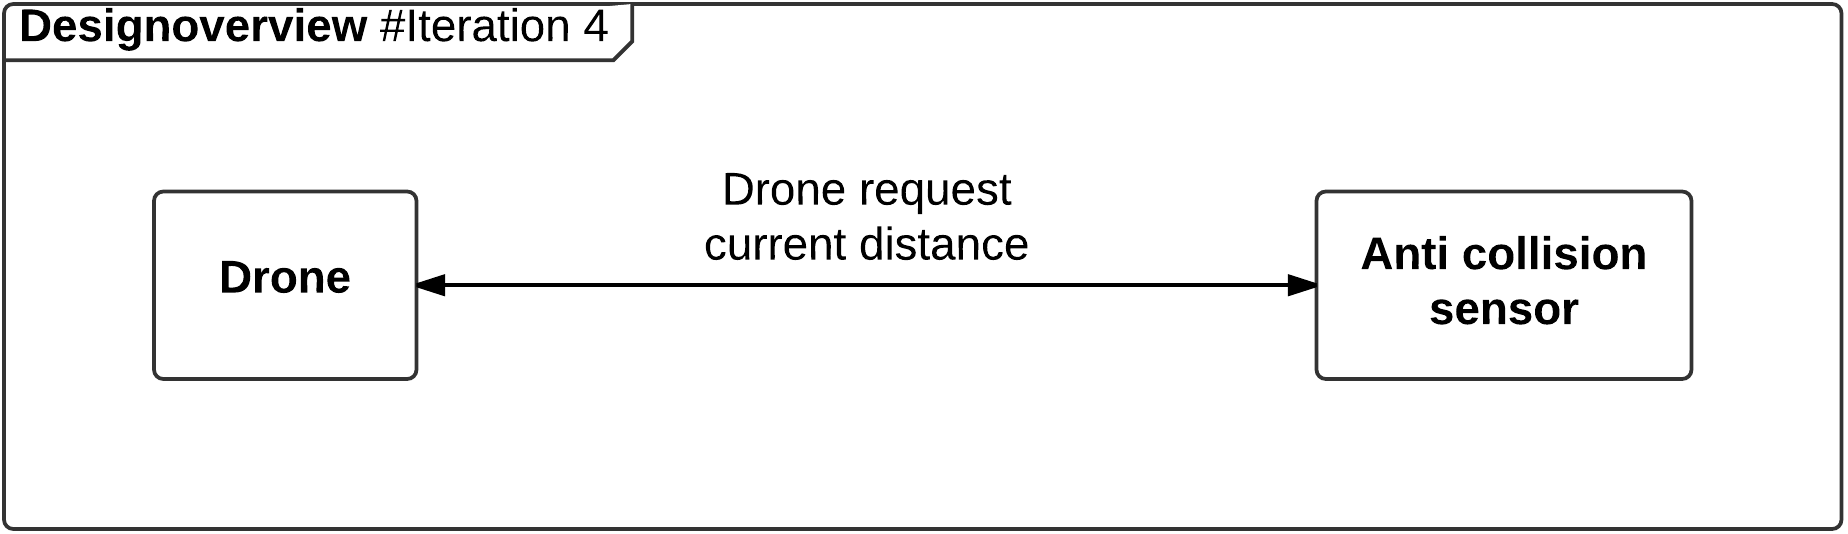
\includegraphics[width=1\textwidth]{Billeder/design_overview/design_overview_iteration4.png}
	\vspace{-.5cm}
	\caption{Designoverview \#iteration 4}
	\label{fig:design_overview_UC4}
\end{figure}


\newpage
\subsubsection*{Sekvens diagram}
\vspace{-0.2cm}
På sekvensdiagrammet vises de klasser der indgår og bruges i fjerde iteration. 
På diagrammet vises det hvordan afstanden til eventuelle objekter foran dronen kontrolleres. Hvis afstanden til et objekt er under den definerede kollisionsgrænse stoppes dronens fremdrift og der skiftes orientering. 


%kommentar
\begin{figure}[H]
	\centering
	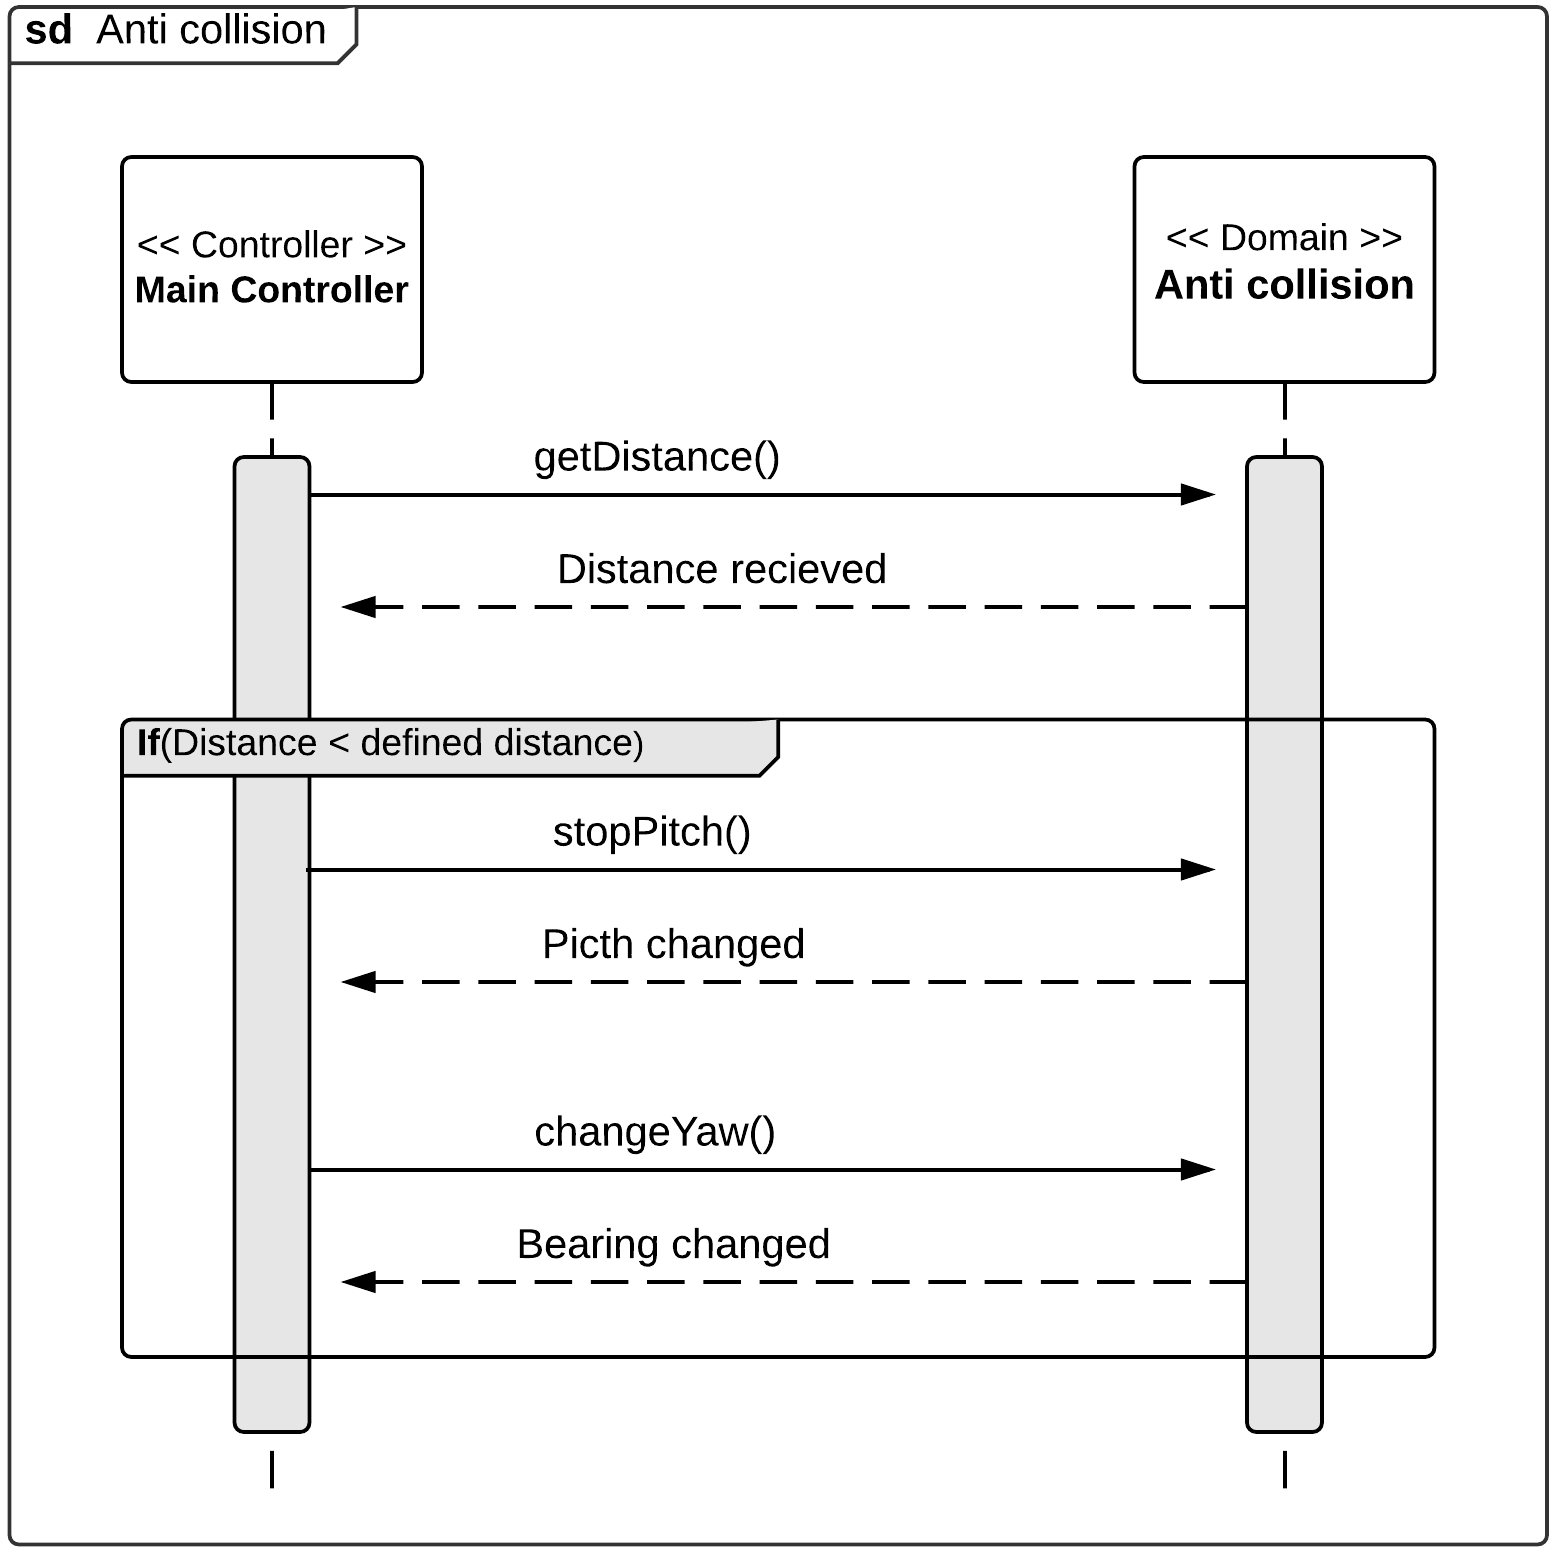
\includegraphics[width=0.8\textwidth]{Billeder/sekvens/sekvens_iteration4}
	\caption{Sekvens diagram \#iteration 4}
	\label{fig:Sekvens_diagram_iteration4}
\end{figure}



\subsubsection*{State machine diagram}
\vspace{-0.2cm}

I state machine diagrammet på figur \ref{fig:Statemachine_iteration4}, vises de to states der eksisterer i iteration 4. Desuden vises hvordan flowet imellem de to states ser ud.


%kommentar
\begin{figure}[H]
	\centering
	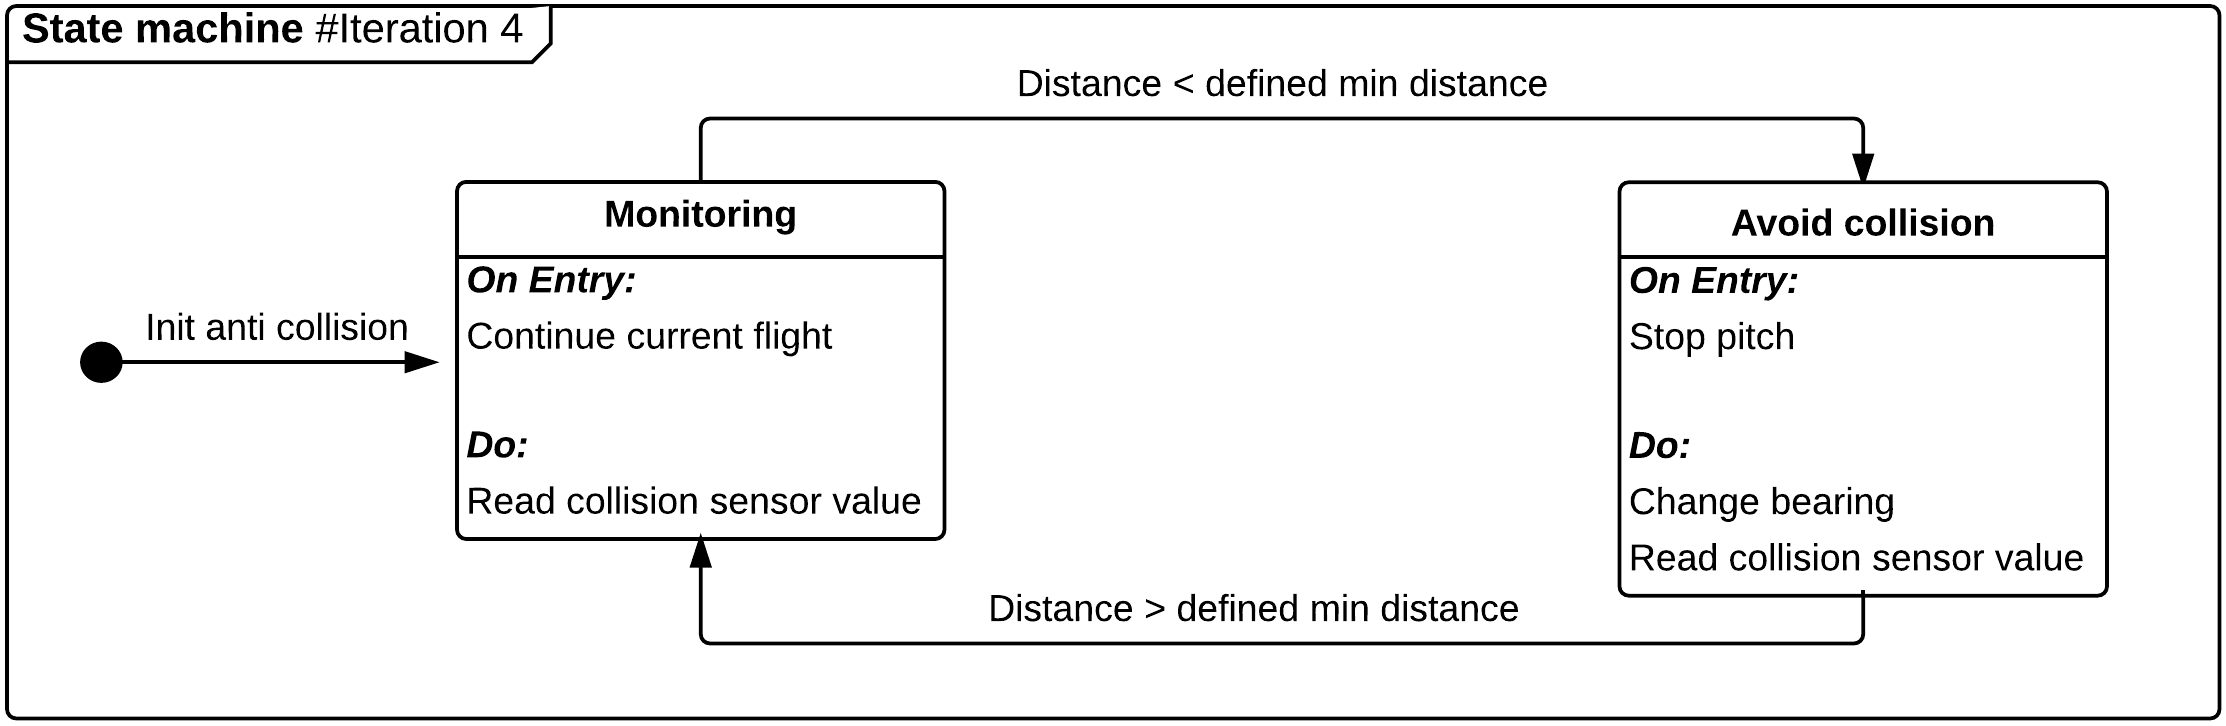
\includegraphics[width=1\textwidth]{Billeder/statemachine/State_iteration4.png}
	\vspace{-0.5cm}
	\caption{Statemachine \#iteration 4}
	\label{fig:Statemachine_iteration4}
\end{figure}



\subsubsection*{Klasse diagram}
\vspace{-0.1cm}

%kommentar
\begin{figure}[H]
	\centering
	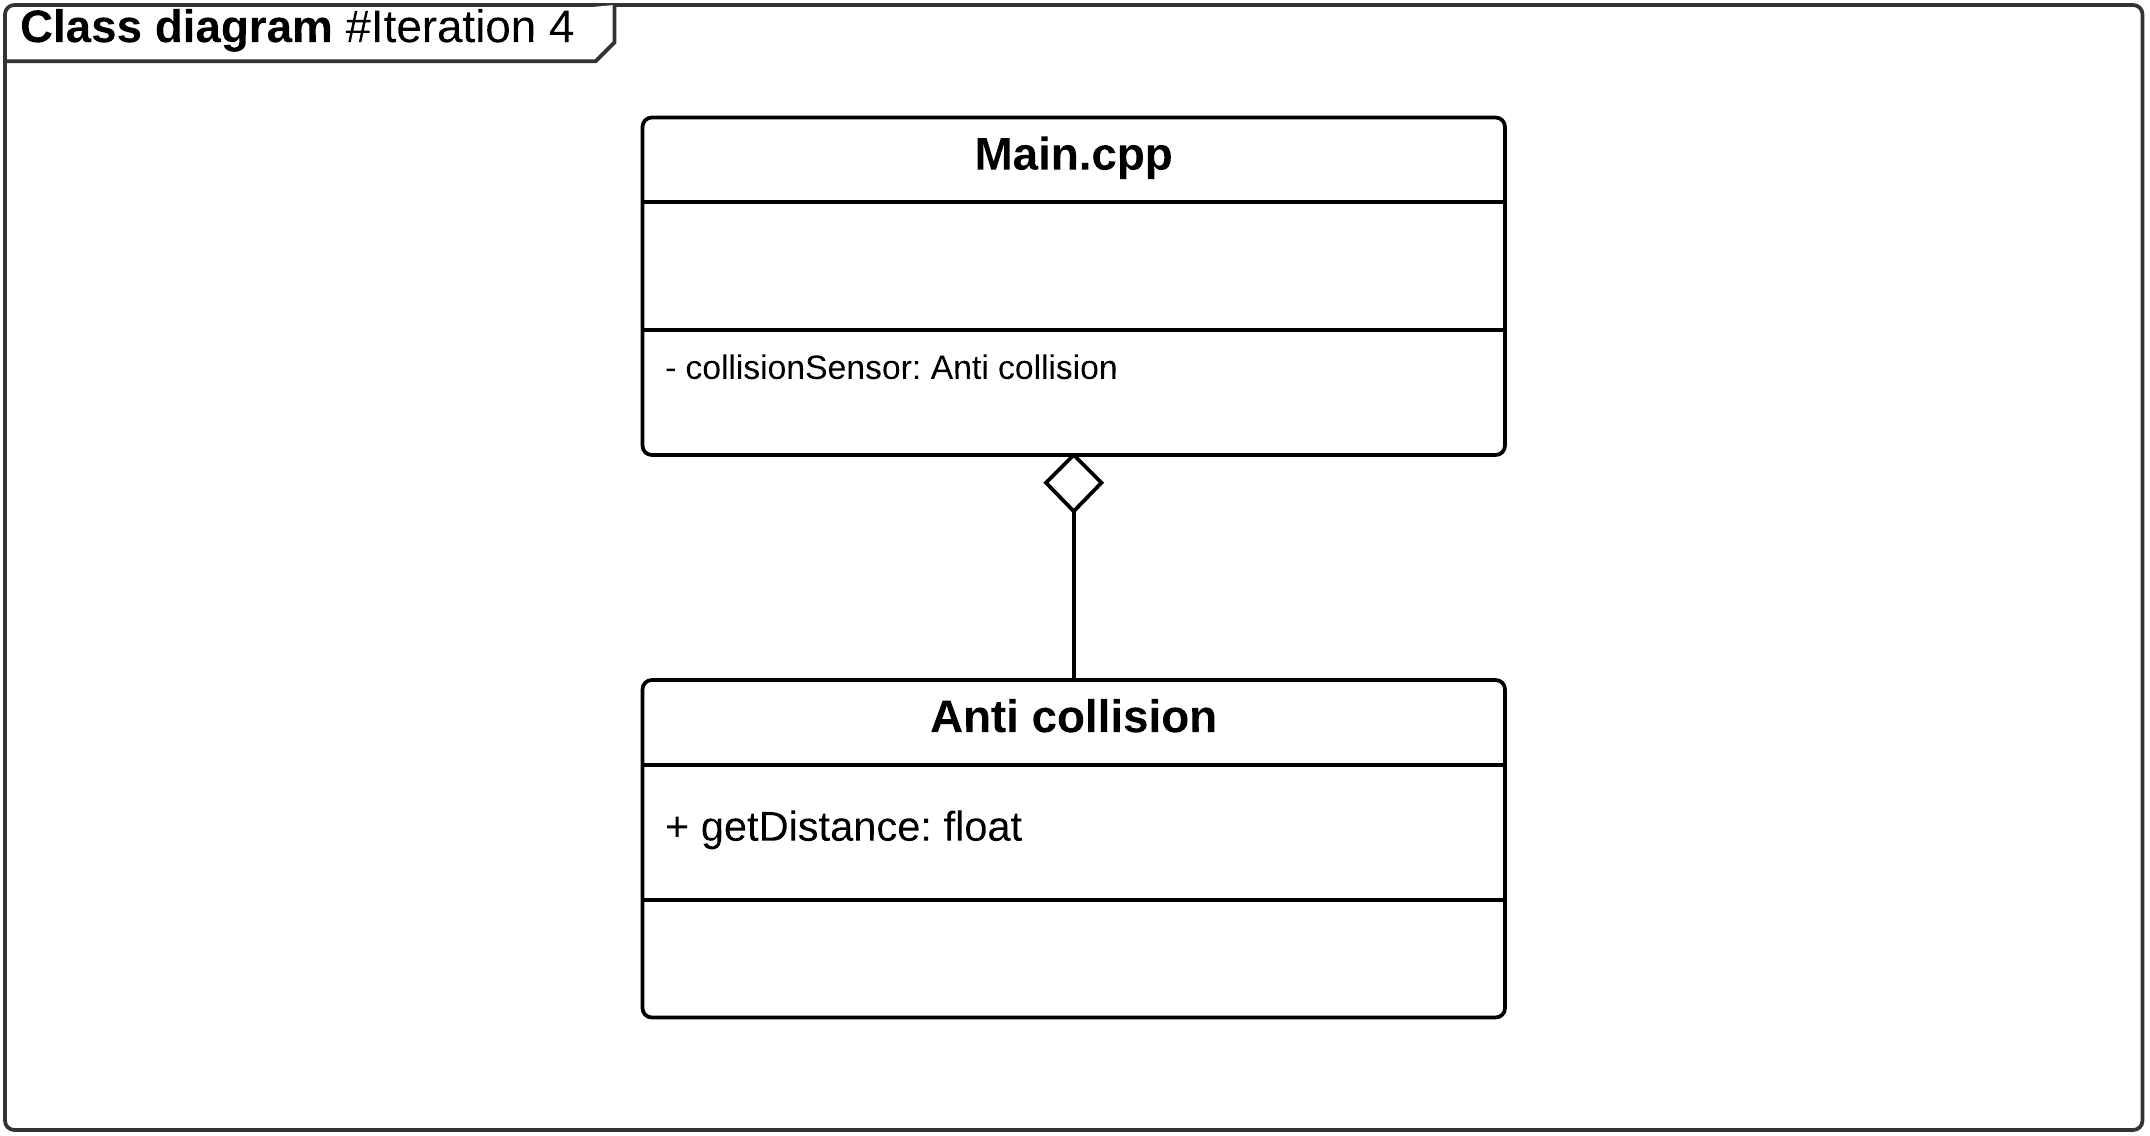
\includegraphics[width=1\textwidth]{Billeder/klasse_diagrammer/classdiagram_iteration4.png}
	\vspace{-0.5cm}
	\caption{Klasse diagram \#iteration 4}
	\label{fig:classDiagram_iteration4}
\end{figure}


\textbf{Main.cpp} \\
Main.cpp filen bruges til at sætte arduino board korrekt op, bla. sættes baudrate på de forskellige serielle forbindelser. Desuden bruges Main.cpp til at kalde og eksekverer forskellige klasse, objekter og funktioner.


\textbf{Anti collision} \\
Module\_3G er ansvarlig for alt kommunikation mellem drone og server. I klassen bruges to forskellige slags http request. Når der ønskes at trække information fra sever til drone gøres der brug af GET request mens der gøres brug af PUT request når dronen ønsker at informere server om ny lokation.
